% ======================================================================
%  CMIG — Pseudo-3D Heightfield Reconstruction (Elsevier elsarticle)
%  Target: Computerized Medical Imaging and Graphics
% ======================================================================
\PassOptionsToPackage{table,xcdraw}{xcolor}
\documentclass[review]{elsarticle}

\usepackage{lineno,hyperref}
\usepackage{textcomp}
\usepackage{newtxtext}
\usepackage{newtxmath}
\usepackage{gensymb}
\usepackage{amsmath}
\usepackage{enumitem}
\DeclareMathOperator*{\argmin}{arg\,min}
\usepackage{graphicx}
  \DeclareGraphicsExtensions{.pdf,.png,.jpg,.jpeg}
\graphicspath{{../figures/}{figures/}{../re3d_cmpb_results/figures/}{pictures/}{images/}{./}}
\usepackage{booktabs}
\usepackage{multirow}
\usepackage{natbib}
\usepackage{subcaption}
\usepackage{tabularx}
\usepackage{tikz}
\usetikzlibrary{arrows.meta,positioning,shapes.geometric,fit,backgrounds,calc,shadows.blur}
\usepackage{etoolbox}
\usepackage{array}

\modulolinenumbers[5]
\setlength{\emergencystretch}{2em}
\sloppy
\makeatletter
\pdfstringdefDisableCommands{%
  \def\corref#1{}%
  \def\cortext#1#2{}%
  \def\@corref#1{}%
  \def\cnotenum#1{}%
}
\makeatother

\journal{Computerized Medical Imaging and Graphics}

%% Numbered references (Elsevier Vancouver style)
\bibliographystyle{elsarticle-num}

\begin{document}

\begin{frontmatter}

\title{Pseudo-3D Heightfield Reconstruction from Monocular Endoscopic Video via Gradient-Anchored Geometric Constraints}

\author[mymainaddress]{Ranyang Li\corref{mycorrespondingauthor}}
\ead{lry@haut.edu.cn}
\author[mymainaddress]{Wufeng Liu}
\author[mymainaddress]{Xiaodong Guo}
\author[mymainaddress]{Chao Fan}
\author[mysecondaryaddress]{Nan Wei}
\author[mythirdaryaddress]{Junjun Pan\corref{mycorrespondingauthor}}
\ead{pan_junjun@buaa.edu.cn}

\cortext[mycorrespondingauthor]{Corresponding authors}

\address[mymainaddress]{School of Artificial Intelligence and Big Data, Henan University of Technology, Zhengzhou 450001, China.}
\address[mysecondaryaddress]{Henan Provincial People's Hospital, Zhengzhou University, Zhengzhou 450003, China.}
\address[mythirdaryaddress]{State Key Laboratory of Virtual Reality Technology and Systems, Beihang University, Beijing 100191, China.}

\begin{highlights}
\item A shared 2.5-D heightfield couples pose estimation and dense matching.
\item Specular-robust gradients keep Normal 3D where learned clouds collapse.
\item Landmarks fix scale and the mask; they are not the reconstructed surface.
\item A stereo variant reaches AbsRel 0.0285 on the EndoNeRF 100-frame set.
\item Confidence-mapped surfaces support overlay and image-guided measurement.
\end{highlights}

\begin{abstract}
Monocular endoscopic reconstruction fails in a specific way: recovered surfaces collapse to cones or planes. Structure-from-motion lacks stable 2D features on specular, texture-poor tissue; feed-forward networks trained on natural images return dense but ill-conditioned geometry. In both cases pose estimation and surface reconstruction do not share a usable 3D signal, so scale and shape cannot be recovered together.
We construct that signal as a gradient-anchored 2.5-D heightfield. Percentile truncation suppresses specular spikes; a region mask keeps the mesh on structurally informative tissue. The same mesh is registered by FPFH--ICP for pose and matched in a 7-D epipolar window for triangulation. Calibration patterns, when visible, fix metric scale and the mask; they are optional anchors, not the reconstructed primitive. If a calibrated stereo pair is available, learned disparity replaces the gradient proxy and the heightfield remains a shape regularizer.
On a chessboard phantom the classical pipeline is the only method that is both Normal\,3D ($\lambda_3/\lambda_1{=}0.42$) and near-metric (scale $1.11{\times}$ versus \texttt{solvePnP}). A 2D essential-matrix pose front-end collapses the same fusion stage to $\lambda_3/\lambda_1{\approx}0.02$. VGGT has a lower ATE ($3.02$ vs.\ $3.89$\,mm) at scale $91{\times}$. A stereo variant reaches median-aligned AbsRel $0.0285$ on a 100-frame EndoNeRF set (FoundationStereo $0.0321$). On SCARED and stereo-laparoscopic data, depth equals SGM by construction; the added product is a confidence-mapped surface. This is not an overall ranking, but a reconstructable surface when shape and scale must be obtained jointly.
\end{abstract}

\begin{keyword}
Endoscopy \sep Reconstruction \sep Visualization \sep Laparoscopy \sep Stereoscopy \sep Heightfield
\end{keyword}

\end{frontmatter}

\linenumbers

% ======================================================================
%  Section 1: Introduction
% ======================================================================
\section{Introduction}
\label{sec:introduction}

Recovering visualizable, metrically scaled 3D surfaces from monocular endoscopic video is a core imaging problem for intra-operative navigation, augmented-reality overlay, and quantitative surgical assessment in minimally invasive surgery (MIS)~\cite{stoyanov2005soft,mountney2010simultaneous}.
Unlike CT or MRI, the endoscope is already in the sterile field and supplies the only continuous intra-operative view; converting that video into a metric surface therefore determines whether graphical overlays and image-guided measurements can be trusted.
A missing or wrong metric scale has direct consequences: estimating the safe instrument-to-tissue standoff that avoids serosal injury, measuring lesion diameter for resection-margin planning, and quantifying tissue deformation during suturing.
These tasks require \emph{metric} (not merely relative) depth, yet most existing pipelines recover only up-to-scale geometry, and the monocular setting removes the baseline cue that stereo reconstruction relies on.
General-purpose 3D vision has advanced rapidly, yet monocular endoscopic reconstruction remains difficult for four reasons.
First, smooth tissue surfaces offer repetitive texture and few discriminative features.
Second, specular reflections from wet tissue violate the photometric consistency that dense reconstruction assumes.
Third, the absence of a physical reference makes the recovered scale ambiguous.
Fourth, reconstructed point clouds often collapse to cones or planes, a geometric degeneracy that no amount of post-hoc rescaling corrects.

Classical structure-from-motion (SfM) methods~\cite{mur2015orbslam,schoenberger2016sfm} fail on such data: on our benchmark COLMAP registers 42 of 50 frames (41 overlap the PnP reference used for ATE) and produces cone-shaped clouds ($\lambda_3/\lambda_1 < 0.13$), and dense SLAM~\cite{newcombe2011dtam,whelan2015elasticfusion} suffers the same specular interference.
Feed-forward networks that perform well on natural images (DUSt3R~\cite{wang2024dust3r}, MASt3R~\cite{leroy2024mast3r}, VGGT~\cite{wang2025vggt}, and Reloc3R~\cite{dong2025reloc3r}) degrade on endoscopic footage: DUSt3R drifts by $647{\times}$ in scale ($\lambda_3/\lambda_1 = 0.09$), VGGT and MASt3R yield flat reconstructions ($\lambda_3/\lambda_1 \leq 0.22$), and Reloc3R does not output point clouds at all.
The cause is a domain gap: networks trained on natural images~\cite{reizenstein2021common} encode matching priors that endoscopic texture and specularities violate.

The thesis of this paper is that the missing quantity is not another depth head, but a \emph{shared, well-conditioned surface embedding}. We construct that embedding as a gradient-anchored 2.5-D heightfield, without learned natural-image priors.
Image gradients, constrained by a region-of-interest mask, encode scene topology: strong responses mark tissue folds and instrument contours, while specular spikes and homogeneous patches are removed by percentile truncation.
The resulting mesh is renderable, and---unlike a disparity map or a set of chessboard corners---it is the same 3D object that subsequent stages consume: FPFH--ICP registers consecutive heightfields to obtain pose, and 7-D epipolar matching queries the same vertices to triangulate a metric cloud (Section~\ref{sec:registration}).
A pose-source ablation isolates this claim: replacing heightfield-ICP poses with a conventional 2D essential-matrix front-end, while keeping the identical fusion stage, collapses the cloud from Normal\,3D to a cone.
Calibration patterns, when present, fix metric scale and define the mask; they are optional anchors rather than the reconstructed primitive~\cite{zhang2000flexible,sturm2001pinhole}. Pose estimation itself does not require landmark detection.

When a calibrated stereo pair is available, a learned disparity network replaces the gradient proxy with metric depth, and the heightfield is retained as a shape regularizer rather than discarded.

The contributions are therefore conceptual rather than a catalogue of modules:
\begin{itemize}[noitemsep,leftmargin=*]
    \item \textbf{Shared surface embedding.} A 2.5-D heightfield is the common geometric substrate for pose and dense matching. The ablation ($\lambda_3/\lambda_1{:}\,0.42\to 0.02$ when the pose front-end is replaced by 2D correspondences) shows that the embedding, not the fusion code, is what prevents cone collapse.
    \item \textbf{Shape as a first-class criterion.} We report $\lambda_3/\lambda_1$ alongside ATE and AbsRel, because a scale-aligned but planar cloud cannot support overlay or measurement. On the chessboard phantom the classical pipeline is the only method that is simultaneously Normal\,3D and near-metric (scale $1.11{\times}$); VGGT is more accurate in ATE and affine-aligned corner depth at scale $91{\times}$.
    \item \textbf{Landmarks as gauge, not primitive.} Prior calibration-pattern methods recover sparse corners. Here the dense surface comes from the heightfield; the pattern, when visible, only sets the metric gauge and the ROI. The same interface accepts a semantic tissue mask when no pattern is present (Section~\ref{sec:pseudo3d}).
    \item \textbf{Optional stereo regularizer.} The classical path remains CPU-only and monocular. The stereo variant reaches median-aligned AbsRel $0.0285$ on a shared 100-frame EndoNeRF set. On SCARED and stereo-laparoscopic data, depth equals SGM by construction; the added output is a confidence-mapped surface. Cross-hardware sequences confirm the scale pattern on two recordings and document collapse on two others.
\end{itemize}

Table~\ref{tab:capability} compares the proposed method with representative approaches on dense reconstruction, metric scale, 3D shape, and CPU-only operation.

\begin{table}[tbp]
\centering
\caption{
    Capability comparison of 3D reconstruction methods on endoscopic data.
    \checkmark: fully supported; $\triangle$: partially supported or limited; $\times$: not supported.
    The classical variant is CPU-only and recovers metric scale when geometric anchors are available (the calibrated stereo variant in Section~\ref{sec:e2e_stereo} requires a GPU for training and inference).
    The 2.5-D heightfield representation has inherent limitations for predominantly lateral motions (Section~\ref{sec:endonerf}).
}
\label{tab:capability}
\setlength{\tabcolsep}{2.5pt}
\renewcommand{\arraystretch}{1.1}
\begin{tabular}{lccccc}
\toprule
Capability & ORB-SfM & COLMAP & VGGT & DUSt3R & \textbf{Ours} \\
\midrule
Dense recon. & $\times$ & $\times$ & \checkmark & \checkmark & $\triangle$ \\
Metric scale & $\triangle$ & $\times$ & $\times$ & $\times$ & \checkmark \\
Normal 3D shape & $\times$ & $\times$ & $\times$ & $\times$ & $\triangle$ \\
Specular robust. & $\times$ & $\times$ & $\triangle$ & $\triangle$ & $\triangle$ \\
No GPU needed & \checkmark & \checkmark & $\times$ & $\times$ & \checkmark \\
Repetitive texture & $\times$ & $\times$ & $\times$ & $\times$ & $\triangle$ \\
\bottomrule
\end{tabular}
\end{table}

% ======================================================================
%  Section 2: Related Work
% ======================================================================
\section{Related Work}
\label{sec:related}

Our research is related to endoscopic 3D reconstruction and visualization, classical and learning-based structure-from-motion, and calibration-pattern-assisted methods in medical imaging. We briefly review representative works in each of these categories.

\textbf{Endoscopic 3D reconstruction.}
Early work on endoscopic 3D reconstruction focused on stereo endoscopes~\cite{stoyanov2005soft,mountney2010simultaneous}, which provide direct depth from binocular disparity, but most surgical endoscopes are monocular.
Shape-from-shading (SfS)~\cite{horn1989shape} recovers surface orientation under Lambertian assumptions but fails under the non-Lambertian reflections prevalent in wet tissue.
Structure-from-motion approaches~\cite{stoyanov2010real} rely on feature correspondences but yield sparse reconstructions in texture-poor images.
Learning-based monocular depth estimation~\cite{eigen2014depth,ranftl2021vision} generalizes poorly to endoscopic scenes; recent surgical methods~\cite{ozyoruk2021endoslam} incorporate temporal consistency and surgical priors yet still produce only relative depth.
Classical stereo matching, in particular semi-global matching (SGM)~\cite{hirschmuller2008sgm}, recovers dense disparity from rectified stereo pairs and remains a strong, training-free baseline for endoscopic depth when a stereo endoscope is available; we therefore adopt it as both a depth source and a comparison baseline throughout this paper.
Reconstructed surfaces are useful only if they can be rendered and registered: prior work on intra-operative augmented reality and image-guided intervention~\cite{mourgues2002calibration,stoyanov2005soft} therefore treats visualization quality---well-formed rather than collapsed geometry---as a requirement, not a post-processing detail.

\textbf{Classical structure-from-motion.}
ORB-SLAM~\cite{mur2015orbslam} uses ORB features~\cite{rublee2011orb} for real-time tracking; COLMAP~\cite{schoenberger2016sfm} employs SIFT~\cite{lowe2004distinctive} with incremental reconstruction and bundle adjustment; LSD-SLAM~\cite{engel2014lsd} performs direct semi-dense reconstruction.
All three rely on discriminative features or photometric consistency, both scarce in endoscopic scenes.
Dense SLAM (DTAM~\cite{newcombe2011dtam}, ElasticFusion~\cite{whelan2015elasticfusion}) similarly requires sufficient texture.
RGB-D methods (KinectFusion~\cite{newcombe2011kinectfusion}, BundleFusion~\cite{dai2017bundlefusion}) are inapplicable to monocular endoscopy.

\textbf{Feed-forward 3D reconstruction networks.}
DUSt3R~\cite{wang2024dust3r} predicts dense stereo pointmaps with global alignment optimization; MASt3R~\cite{leroy2024mast3r} extends DUSt3R with local feature matching and metric pointmaps; MUSt3R~\cite{cabon2025must3r} extends DUSt3R to multi-view settings with a memory network; VGGT~\cite{wang2025vggt} jointly predicts poses, depth, and point clouds via a Vision Geometry Grounded Transformer; Reloc3R~\cite{dong2025reloc3r} adapts DUSt3R for camera relocalization.
Separately, coordinate-based methods (NeRF~\cite{mildenhall2021nerf}, 3D Gaussian Splatting~\cite{kerbl2023gaussian}) achieved photorealistic novel view synthesis but require per-scene optimization and dense input views.
Multi-view stereo networks (MVSNet~\cite{yao2018mvsnet} and successors~\cite{yi2020pyramidmvs}) require known camera poses and struggle with texture-poor regions.
As shown in Section~\ref{sec:results}, all feed-forward methods produce degenerate point clouds on endoscopic data due to the domain gap between natural-image training sets and endoscopic imaging conditions.

\textbf{Calibration-pattern-based methods in medical imaging.}
Chessboard calibration patterns are widely used for camera calibration~\cite{zhang2000flexible,sturm2001pinhole}, instrument tracking~\cite{zhao2017real}, and AR overlay~\cite{mourgues2002calibration}.
Previous work uses chessboard corners as sparse landmarks for pose estimation and scale recovery~\cite{zhao2017real,mourgues2002calibration}, yielding only sparse 3D information.
In contrast, we exploit calibration patterns as \emph{geometric anchors} that constrain the \emph{dense} reconstruction pipeline, from heightfield construction and pose estimation to dense matching and metric fusion.

\textbf{Summary of gaps.}
Taken together, dense, metric-scale, and geometrically well-formed reconstruction from monocular endoscopic video is still not available from a single CPU-only method.
Classical SfM yields sparse or degenerate clouds when features are scarce; feed-forward networks remain dense but collapse geometrically on this domain; and prior calibration-pattern methods recover only sparse landmarks.
The gradient-anchored heightfield is designed for that joint requirement: pose and matching share one well-conditioned surface, while calibration patterns set the metric gauge rather than supplying the reconstructed geometry.

% ======================================================================
%  Section 3: Method
% ======================================================================
\section{Method}
\label{sec:method}

\subsection{Problem Formulation}
\label{sec:problem}

Given a monocular endoscopic video sequence $\{I_t\}_{t=0}^{N-1}$ of $N$ frames, our goal is to recover a dense, metrically scaled 3D point cloud $\mathcal{P} = \{(\mathbf{X}_k, \mathbf{c}_k)\}_{k=1}^{K}$ of the surgical scene, where $\mathbf{X}_k \in \mathbb{R}^3$ denotes a 3D point and $\mathbf{c}_k \in [0,255]^3$ its associated color.
The reconstructed cloud, together with the per-frame heightfield mesh and an optional confidence map, is intended as a visualizable geometric layer for intra-operative graphics and image-guided measurement.
When a planar calibration pattern (e.g., a chessboard marker) with known geometry is present, it provides optional geometric anchors that constrain the pipeline, as detailed in the following sections.

\paragraph{Notation.}
We denote camera poses as $\mathbf{T}_t \in \mathrm{SE}(3)$ (camera-to-world), the camera intrinsic matrix as $\mathbf{K} \in \mathbb{R}^{3\times3}$, and the chessboard corner set as $\{\mathbf{u}_{t,k}\}_{k=1}^{M}$ for frame $t$.
The coordinate system uses $(u,v)$ for pixel coordinates and $h$ for the pseudo-height derived from image gradients.
Table~\ref{tab:notation} summarizes the notation used throughout this paper.

\begin{table}[tbp]
\centering
\caption{Summary of notation.}
\label{tab:notation}
\setlength{\tabcolsep}{1.5pt}
\renewcommand{\arraystretch}{1.0}
\begin{tabular}{ll}
\toprule
Symbol & Definition \\
\midrule
$I_t$ & Input image at frame $t$, $I_t \in \mathbb{R}^{H\times W\times 3}$ \\
$\mathbf{T}_t$ & Camera-to-world pose, $\mathbf{T}_t \in \mathrm{SE}(3)$ \\
$\mathbf{R}_t, \mathbf{t}_t$ & Rotation and translation of $\mathbf{T}_t$ \\
$\mathbf{K}$ & Camera intrinsic matrix, $\mathbf{K} \in \mathbb{R}^{3\times3}$ \\
$\mathbf{u}_{t,k}$ & $k$-th detected landmark in frame $t$ (pixels; e.g., calibration pattern corner) \\
$\mathbf{X}_k$ & 3D point in world coordinates (mm) \\
$\mathcal{P}$ & Reconstructed point cloud \\
$M$ & Number of detected landmarks \\
$s_{\mathrm{sq}}$ & Calibration pattern square side length (mm) \\
$g_t(u,v)$ & Gradient magnitude at pixel $(u,v)$ in frame $t$ \\
$\hat{g}_t(u,v)$ & Truncated gradient after percentile thresholding \\
$M_t(u,v)$ & Binary ROI mask (derived from detectable landmarks in our implementation) \\
$\mathcal{H}_t$ & Pseudo-3D heightfield mesh for frame $t$ \\
$\tau_{\%}$ & Gradient percentile threshold (default: 68\%) \\
$c_{\mathrm{cell}}$ & Mesh grid cell size in pixels (default: 3) \\
$z_s$ & Height scaling factor, $z_s = 0.15\max(H,W)$ \\
$\mathbf{f}(u,v)$ & 7D geometric feature at a heightfield vertex \\
$r$ & Dense-matching search radius (default: 25\,px) \\
$\mathbf{F}$ & Fundamental matrix, $\mathbf{F}=\mathbf{K}^{-\top}[\mathbf{t}]_\times\mathbf{R}\,\mathbf{K}^{-1}$ \\
$W_r$ & Matching search window of radius $r$ about the pose-predicted location \\
$\epsilon_{\mathrm{epi}}$ & Epipolar band width (default: 2.0\,px) \\
$\mathbf{P}_i$ & $3{\times}4$ projection matrix of view $i$ \\
$\tau_{\mathrm{reproj}}$ & Reprojection threshold (default: 2.0\,px) \\
$\pi(\cdot)$ & Perspective projection of a 3D point to the image plane \\
$\boldsymbol{\Phi}^{(s)}$ & Multi-scale stereo encoder features at resolution $s$ (distinct from $\mathbf{F}$) \\
$\mathbf{C}$ & Stereo cost volume, $\mathbf{C}\in\mathbb{R}^{D\times H\times W}$ \\
$\lambda_3/\lambda_1$ & PCA shape ratio (Normal\,3D ${\geq}0.25$; Flat $0.15$--$0.25$; Cone ${<}0.15$) \\
\bottomrule
\end{tabular}
\end{table}

\subsection{Pipeline Overview}
\label{sec:overview}

The proposed framework processes monocular endoscopic video through four sequential stages (Fig.~\ref{fig:pipeline}).
First (Section~\ref{sec:pseudo3d}), each frame is converted into a 2.5-D heightfield mesh from truncated image gradients and a region-of-interest mask derived from a calibration pattern or other detectable landmarks when available; the mesh captures the topology of the visible tissue surface and can be rendered directly.
Second (Section~\ref{sec:registration}), inter-frame poses are estimated by registering consecutive heightfields with FPFH coarse alignment (PCA or feature-matched RANSAC) and point-to-point ICP, gated by an online quality measure.
Third (Section~\ref{sec:epipolar}), the estimated poses establish dense correspondences through epipolar-constrained geometric matching on the heightfield.
Fourth (Section~\ref{sec:fusion}), per-frame reconstructions are triangulated and fused into a globally consistent metric point cloud.
When a calibrated stereo pair is available, an optional end-to-end variant (Section~\ref{sec:e2e_stereo}) recovers metric depth through a learned disparity network regularized toward geometrically consistent 3D structure. The classical monocular pipeline remains the primary method.

\begin{figure}[tbp]
\centering
\resizebox{\linewidth}{!}{%
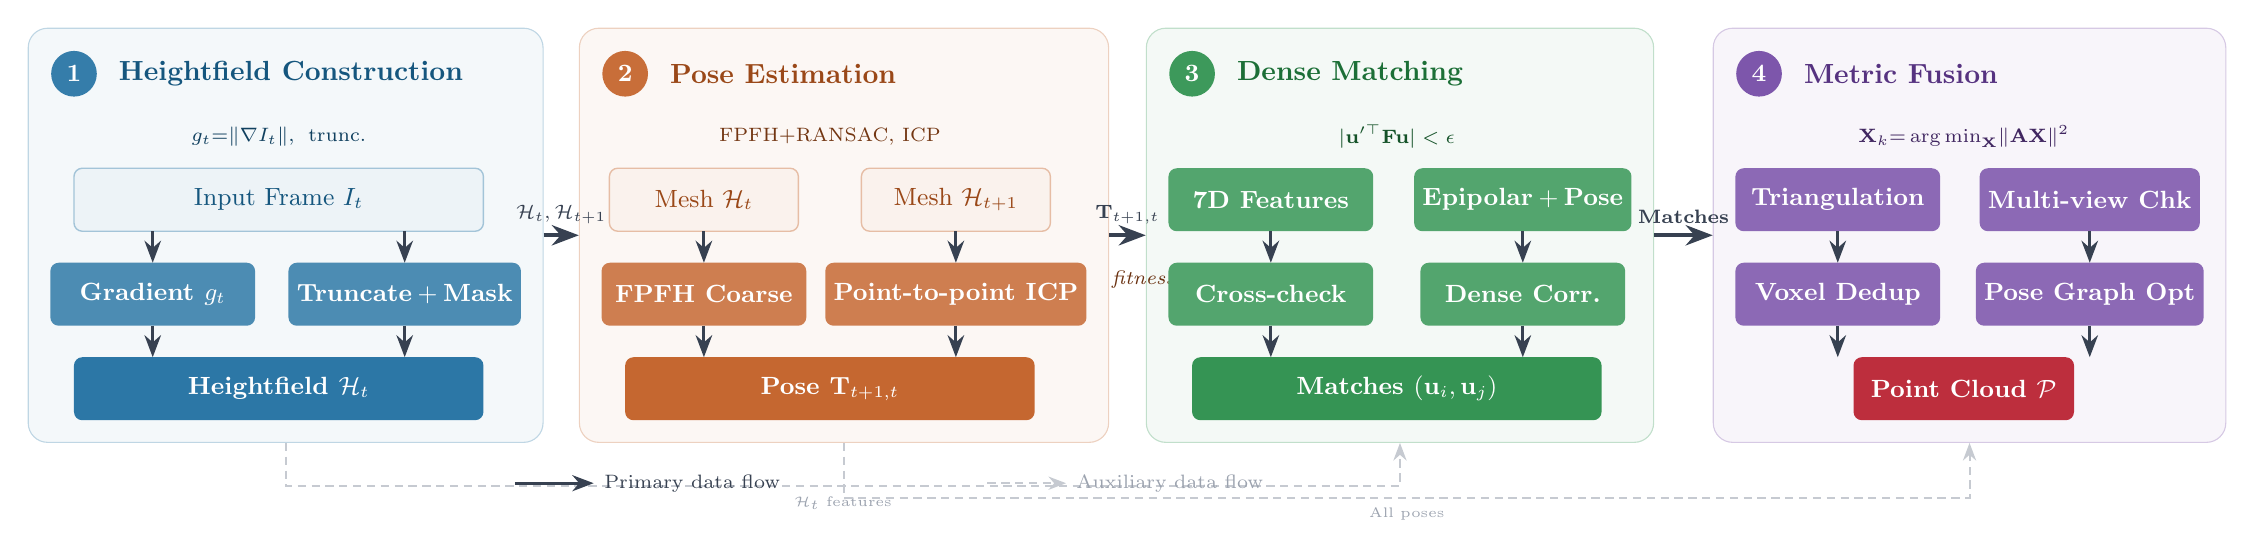
\begin{tikzpicture}[
    >=Stealth,
    % ── Box styles ──
    box/.style={rounded corners=3pt, minimum height=8.0mm, text centered,
                font=\small, inner sep=3pt, outer sep=0pt},
    ibox/.style={box, minimum width=24mm, fill=#1!8, draw=#1!40, line width=0.5pt,
                 text=#1!80!black},
    pbox/.style={box, minimum width=26mm, fill=#1!78, text=white,
                 font=\small\bfseries},
    obox/.style={box, minimum width=28mm, fill=#1!92, text=white,
                 font=\small\bfseries},
    % ── Arrow styles ──
    arr/.style={->, line width=1.1pt, color=#1},
    darr/.style={->, line width=0.75pt, color=#1!58, densely dashed},
    % ── Labels ──
    slbl/.style={font=\normalsize\bfseries, text=#1!80!black},
    numc/.style={circle, fill=#1!88, text=white, font=\small\bfseries,
                 inner sep=0pt, minimum size=5.8mm},
    annot/.style={font=\scriptsize\itshape, text=#1!55!black},
    eqtag/.style={font=\scriptsize, text=#1!60!black, align=center},
]

% ── Color palette ──
\definecolor{c1}{HTML}{1A6B9E}   % Stage 1: deep blue
\definecolor{c2}{HTML}{C05A1E}   % Stage 2: burnt orange
\definecolor{c3}{HTML}{238B45}   % Stage 3: forest green
\definecolor{c4}{HTML}{6B3FA0}   % Stage 4: royal purple
\definecolor{cout}{HTML}{B71C2C} % Output: crimson
\definecolor{carr}{HTML}{374151} % Arrows: dark gray
\definecolor{caux}{HTML}{9CA3AF} % Auxiliary: medium gray

% ═══ Grid layout: 4 stages, y-levels = header(4.3), top(2.7), mid(1.5), bot(0.3) ═══
% ═══ Stage centers at x = 0, 7.0, 14.2, 21.4                                 ═══

% ═══════════════════════════════════════════════════
%  STAGE 1 — Pseudo-3D Heightfield Mesh Construction
% ═══════════════════════════════════════════════════
\node[numc=c1] (n1) at (-2.6, 4.3) {1};
\node[slbl=c1, right=1.5mm of n1] {Heightfield Construction};

\node[ibox=c1, minimum width=52mm] (s1in)  at (0, 2.7) {Input Frame $I_t$};
\node[pbox=c1] (s1grad) at (-1.6, 1.5) {Gradient $g_t$};
\node[pbox=c1] (s1trunc) at (1.6, 1.5) {Truncate $\!+\!$ Mask};
\node[obox=c1, minimum width=52mm] (s1mesh) at (0, 0.3) {Heightfield $\mathcal{H}_t$};

% Stage 1: separate orthogonal arrows (each source→target independently)
\draw[arr=carr] (s1in.south -| s1grad.north) -- (s1grad.north);
\draw[arr=carr] (s1in.south -| s1trunc.north) -- (s1trunc.north);
\draw[arr=carr] (s1grad.south) -- (s1mesh.north -| s1grad.south);
\draw[arr=carr] (s1trunc.south) -- (s1mesh.north -| s1trunc.south);

% ═══════════════════════════════════════════════════
%  STAGE 2 — Heightfield-Based Pose Estimation
% ═══════════════════════════════════════════════════
\node[numc=c2] (n2) at (4.4, 4.3) {2};
\node[slbl=c2, right=1.5mm of n2] {Pose Estimation};

\node[ibox=c2] (s2mt)  at (5.4, 2.7) {Mesh $\mathcal{H}_t$};
\node[ibox=c2] (s2mt1) at (8.6, 2.7) {Mesh $\mathcal{H}_{t+1}$};
\node[pbox=c2] (s2svd) at (5.4, 1.5) {FPFH Coarse};
\node[pbox=c2] (s2icp) at (8.6, 1.5) {Point-to-point ICP};
\node[obox=c2, minimum width=52mm] (s2pose) at (7.0, 0.3) {Pose $\mathbf{T}_{t+1,t}$};

% Stage 2: separate orthogonal arrows
\draw[arr=carr] (s2mt.south)  -- (s2svd.north);
\draw[arr=carr] (s2mt1.south) -- (s2icp.north);
\draw[arr=carr] (s2svd.south) -- (s2pose.north -| s2svd.south);
\draw[arr=carr] (s2icp.south) -- (s2pose.north -| s2icp.south);
\node[annot=c2, above right=-0.5mm and 2mm of s2icp.east] {fitness gate};

% ═══════════════════════════════════════════════════
%  STAGE 3 — Dense Epipolar Matching
% ═══════════════════════════════════════════════════
\node[numc=c3] (n3) at (11.6, 4.3) {3};
\node[slbl=c3, right=1.5mm of n3] {Dense Matching};

\node[pbox=c3] (s3feat) at (12.6, 2.7) {7D Features};
\node[pbox=c3] (s3epi)  at (15.8, 2.7) {Epipolar $\!+\!$ Pose};
\node[pbox=c3] (s3xchk) at (12.6, 1.5) {Cross-check};
\node[pbox=c3] (s3dense) at (15.8, 1.5) {Dense Corr.};
\node[obox=c3, minimum width=52mm] (s3match) at (14.2, 0.3) {Matches $(\mathbf{u}_i,\mathbf{u}_j)$};

% Stage 3: separate orthogonal arrows
\draw[arr=carr] (s3feat.south) -- (s3xchk.north);
\draw[arr=carr] (s3epi.south)  -- (s3dense.north);
\draw[arr=carr] (s3xchk.south) -- (s3match.north -| s3xchk.south);
\draw[arr=carr] (s3dense.south) -- (s3match.north -| s3dense.south);

% ═══════════════════════════════════════════════════
%  STAGE 4 — Multi-Frame Metric Fusion
% ═══════════════════════════════════════════════════
\node[numc=c4] (n4) at (18.8, 4.3) {4};
\node[slbl=c4, right=1.5mm of n4] {Metric Fusion};

\node[pbox=c4] (s4tri) at (19.8, 2.7) {Triangulation};
\node[pbox=c4] (s4mv)  at (23.0, 2.7) {Multi-view Chk};
\node[pbox=c4] (s4vox) at (19.8, 1.5) {Voxel Dedup};
\node[pbox=c4] (s4pg)  at (23.0, 1.5) {Pose Graph Opt};
\node[obox=cout] (s4out) at (21.4, 0.3) {Point Cloud $\mathcal{P}$};

% Stage 4: separate orthogonal arrows
\draw[arr=carr] (s4tri.south) -- (s4vox.north);
\draw[arr=carr] (s4mv.south)  -- (s4pg.north);
\draw[arr=carr] (s4vox.south) -- (s4out.north -| s4vox.south);
\draw[arr=carr] (s4pg.south)  -- (s4out.north -| s4pg.south);

% ═══════════════════════════════════════════════════
%  CORE EQUATION ANNOTATIONS
% ═══════════════════════════════════════════════════
\node[eqtag=c1] at (0, 3.5) {$g_t{=}\lVert\nabla I_t\rVert$, \;trunc.};
\node[eqtag=c2] at (7.0, 3.5) {FPFH$+$RANSAC, ICP};
\node[eqtag=c3] at (14.2, 3.5) {$|\mathbf{u}'^\top\mathbf{F}\mathbf{u}|<\epsilon$};
\node[eqtag=c4] at (21.4, 3.5) {$\mathbf{X}_k{=}\argmin_{\mathbf{X}}\lVert\mathbf{A}\mathbf{X}\rVert^2$};

% ═══════════════════════════════════════════════════
%  STAGE BACKGROUND PANELS (named, include ALL nodes)
% ═══════════════════════════════════════════════════
\begin{scope}[on background layer]
  \node[fit=(n1)(s1in)(s1grad)(s1trunc)(s1mesh), fill=c1!5, draw=c1!28,
        rounded corners=7pt, inner sep=8pt] (panel1) {};
  \node[fit=(n2)(s2mt)(s2mt1)(s2svd)(s2icp)(s2pose), fill=c2!5, draw=c2!28,
        rounded corners=7pt, inner sep=8pt] (panel2) {};
  \node[fit=(n3)(s3feat)(s3epi)(s3xchk)(s3dense)(s3match), fill=c3!5, draw=c3!28,
        rounded corners=7pt, inner sep=8pt] (panel3) {};
  \node[fit=(n4)(s4tri)(s4mv)(s4vox)(s4pg)(s4out), fill=c4!5, draw=c4!28,
        rounded corners=7pt, inner sep=8pt] (panel4) {};
\end{scope}

% ═══════════════════════════════════════════════════
%  CROSS-STAGE DATA FLOW (connect panel-to-panel borders)
% ═══════════════════════════════════════════════════
\draw[arr=carr, line width=1.5pt]
    (panel1.east) -- node[above, font=\scriptsize\bfseries, text=carr] {$\mathcal{H}_t,\mathcal{H}_{t+1}$} (panel2.west);

\draw[arr=carr, line width=1.5pt]
    (panel2.east) -- node[above, font=\scriptsize\bfseries, text=carr] {$\mathbf{T}_{t+1,t}$} (panel3.west);

\draw[arr=carr, line width=1.5pt]
    (panel3.east) -- node[above, font=\scriptsize\bfseries, text=carr] {Matches} (panel4.west);

% ═══════════════════════════════════════════════════
%  AUXILIARY DATA FLOW (dashed, routed orthogonally)
% ═══════════════════════════════════════════════════
\draw[darr=caux]
    (panel1.south) -- ++(0,-0.55) -|
    node[pos=0.25, below, font=\tiny, text=caux] {$\mathcal{H}_t$ features} (panel3.south);

\draw[darr=caux]
    (panel2.south) -- ++(0,-0.70) -|
    node[pos=0.25, below, font=\tiny, text=caux] {All poses} (panel4.south);

% ═══════════════════════════════════════════════════
%  LEGEND
% ═══════════════════════════════════════════════════
\draw[arr=carr, line width=1.05pt] (3.0, -0.90) -- (4.0, -0.90)
    node[right, font=\scriptsize, text=carr] {Primary data flow};
\draw[darr=caux] (9.0, -0.90) -- (10.0, -0.90)
    node[right, font=\scriptsize, text=caux] {Auxiliary data flow};

\end{tikzpicture}%
}%
\caption{Overview of the proposed pseudo-3D reconstruction pipeline. Four colour-coded stages process monocular endoscopic video into a metric point cloud.\
\textbf{Stage~1 (Gradient-based heightfield construction):} percentile truncation and ROI masking convert input frames into a heightfield mesh; the core gradient operator is $g_t{=}\lVert\nabla I_t\rVert$.\
\textbf{Stage~2 (Heightfield-based pose estimation):} FPFH-feature coarse alignment (PCA or RANSAC), point-to-point ICP, and online quality gating.\
\textbf{Stage~3 (Dense epipolar matching):} 7D geometric features with pose-predicted search windows and epipolar constraint ($|\mathbf{u}'^\top\mathbf{F}\mathbf{u}|<\epsilon$).\
\textbf{Stage~4 (Multi-frame metric fusion):} triangulation ($\mathbf{X}_k{=}\argmin\lVert\mathbf{A}\mathbf{X}\rVert^2$), multi-view consistency filtering, voxel deduplication, and pose graph optimization.\
\textbf{Legend:} numbered circles denote stage index; light boxes are inputs, filled boxes are processing steps, dark boxes are outputs; solid arrows denote primary data flow; dashed arrows denote auxiliary data flow (features, poses); equation annotations summarise the core operation of each stage.}
\label{fig:pipeline}
\end{figure}

\subsection{Pseudo-3D Heightfield Mesh Construction}
\label{sec:pseudo3d}

Image gradients encode the topological structure of the surgical scene: strong gradients mark structural edges, while weak gradients from homogeneous regions are suppressed by percentile truncation.

\paragraph{Gradient computation and truncation.}
For each frame $I_t$ of spatial resolution $H \times W$ (rows $\times$ columns), we compute the gradient magnitude map:
\begin{equation}
    g_t(u,v) = \left\|\nabla I_t(u,v)\right\|
    = \sqrt{\left(\frac{\partial I_t}{\partial u}\right)^{\!2} + \left(\frac{\partial I_t}{\partial v}\right)^{\!2}}.
    \label{eq:gradient}
\end{equation}
To suppress noise and spurious gradients from specular reflections, we apply percentile-based truncation:
\begin{equation}
    \hat{g}_t(u,v) = \begin{cases}
        g_t(u,v), & \text{if } g_t(u,v) \geq \tau_g, \\
        0, & \text{otherwise},
    \end{cases}
    \label{eq:truncation}
\end{equation}
where $\tau_g = \mathrm{Perc}_{\tau_{\%}}(g_t)$ denotes the $\tau_{\%}$-th percentile of the gradient distribution.
With $\tau_{\%}=68$, the upper portion of the gradient distribution is retained; this operating point sits on the flat region of the sensitivity curve in Supplementary Material, Section~D.
A sensitivity analysis across $\tau_{\%} \in [30,90]$ is provided in the Supplementary Material, Section~D.

\paragraph{Region-of-interest mask.}
When detectable landmarks such as a calibration pattern are present, they provide a binary region-of-interest mask $M_t(u,v) \in \{0,1\}$ (e.g., detected via standard corner detection~\cite{bradski2000opencv} for chessboard patterns).
The mask serves two purposes:
(1)~it suppresses background regions that would otherwise dominate the heightfield and corrupt ICP convergence; and
(2)~it defines the reliable region for subsequent pose quality evaluation.
The truncated gradient map is further masked:
\begin{equation}
    \tilde{g}_t(u,v) = \hat{g}_t(u,v) \cdot M_t(u,v).
    \label{eq:mask}
\end{equation}
This masking ensures that only gradient responses within the region of interest contribute to the heightfield, removing the influence of irrelevant tissue and instrument regions.
The interface is deliberately source-agnostic: $M_t$ may come from a chessboard hull, a contour fallback, or a semantic tissue probability in $[0,1]$. Instruments and specular blobs should be excluded from the tissue heightfield rather than reconstructed as a second depth layer, which a single 2.5-D mesh cannot represent.

\paragraph{Heightfield mesh generation.}
The masked gradient map $\tilde{g}_t$ (normalised to $[0,255]$) is lifted to a 2.5-D heightfield mesh $\mathcal{H}_t$ by constructing a regular grid with cell size $c_{\mathrm{cell}}$ pixels (default: 3).
Each grid vertex $(u,v)$ is assigned a height value:
\begin{equation}
    h(u,v) = z_s \cdot \frac{\tilde{g}_t(u,v)}{255},
    \label{eq:height}
\end{equation}
where $z_s$ is the height scaling factor, set to $z_s = 0.15\,\max(H,W)$ (a fixed fraction of the image extent) so that the maximum height is comparable to the image dimensions, ensuring that the heightfield has comparable horizontal and vertical scales for ICP convergence.
Adjacent vertices are connected via a regular grid triangulation (each grid cell is split into two triangles), yielding a manifold surface $\mathcal{H}_t = (\mathcal{V}_t, \mathcal{F}_t)$ with $|\mathcal{V}_t| \approx HW / c_{\mathrm{cell}}^2$ vertices.

\subsection{Inter-Frame Registration and Dense Reconstruction}
\label{sec:registration}

The relative transformation between consecutive frames is estimated by registering their pseudo-3D heightfield meshes through a multi-stage ICP pipeline.

\paragraph{Feature-based coarse alignment.}
The two heightfield meshes $\mathcal{H}_t$ and $\mathcal{H}_{t+1}$ are first converted to point clouds and a coarse rigid alignment is estimated in two stages, so that the subsequent refinement starts close to the optimum and avoids convergence to local minima, which is common in texture-poor endoscopic scenes where an identity or random initialization often fails.
First, surface normals are estimated by a KD-tree search and each point is described by a Fast Point Feature Histogram (FPFH)~\cite{rusu2009fpfh}, a 33-dimensional histogram of the local surface geometry that is robust to the weak texture and specular highlights typical of endoscopic imagery.
Coarse registration then proceeds by attempting, in order, (i)~a principal-axis (PCA) alignment that rotates the clouds so their principal axes coincide and recenters them at their centroids, and (ii)~if the PCA alignment residual exceeds $10\%$ of the cloud scale, a global RANSAC registration driven by FPFH feature matching:
\begin{equation}
    \mathbf{T}_0 = \argmin_{\mathbf{T}} \; \sum_{(i,j)\in\mathcal{C}} \left\|\mathbf{T}\,\mathbf{p}_{t,i} - \mathbf{q}_{t+1,j}\right\|^2,
    \label{eq:ransac}
\end{equation}
where $\mathcal{C}$ is the FPFH-feature correspondence set produced by the RANSAC hypothesis-and-test loop (with a $5{\times}$-enlarged correspondence distance and a minimum-fitness gate of $0.1$), $\mathbf{p}_{t,i}$ and $\mathbf{q}_{t+1,j}$ are source (frame $t$) and target (frame $t{+}1$) heightfield points forming a correspondence in $\mathcal{C}$, and $\mathbf{T}_0$ is the transformation with the largest inlier support.
This feature-driven coarse stage replaces a landmark-based initializer: it does not require detected corners or a calibration pattern, and it operates directly on the 3D surface geometry of the heightfield, which is the same signal the refinement and fusion stages consume.

\paragraph{Point-to-point ICP refinement.}
Starting from the coarse alignment $\mathbf{T}_0$, the transformation is refined with point-to-point ICP~\cite{besl1992icp}.
The source and target clouds are voxel-downsampled to a target point budget (so that the per-pair cost stays bounded on large frames), and the least-squares objective
\begin{equation}
    \mathbf{T}_{t+1,t} = \argmin_{\mathbf{T}} \; \sum_{i} \left\|\mathbf{T}\,\mathbf{p}_{t,i} - \mathbf{q}_{t+1,\mathcal{N}(i)}\right\|^2,
    \label{eq:icp}
\end{equation}
is minimised, where $\mathbf{p}_{t,i}$ is a source point, $\mathcal{N}(i)$ denotes its nearest-neighbour index in the target cloud, and $\mathbf{q}_{t+1,\mathcal{N}(i)}$ is the corresponding target point.
The correspondence distance is set adaptively from the cloud scale and shrunk as the registration converges. Point-to-point ICP (Eq.~\eqref{eq:icp}) is used here because the heightfield is a smooth surface whose normals are dominated by the gradient proxy rather than true surface normals; a point-to-plane variant would over-weight the unreliable normal direction, and the empirical comparison (Section~\ref{sec:ablation}) shows the point-to-point objective already yields the Normal\,3D geometry, so the added complexity of a robust kernel is unnecessary for this representation.

\paragraph{Quality gating and recovery.}
After ICP convergence, the registration quality is gated by the ICP overlap fitness: a transform is accepted when fitness exceeds $0.3$ after a successful coarse alignment, or $0.1$ on the RANSAC/centroid fallback branch, and is otherwise rejected and re-initialised.
When detectable landmarks (e.g., calibration-pattern corners) are available, an additional, optional landmark-based validation is performed by the reprojection residual. Write the estimated relative pose as
$\mathbf{T}_{t+1,t}=\begin{bmatrix}\mathbf{R}&\mathbf{t}\\\mathbf{0}^{\top}&1\end{bmatrix}$,
which maps coordinates of frame $t$ into frame $t{+}1$. For a 3D landmark $\mathbf{X}_k$ expressed in frame $t$ and its observation $\mathbf{u}_{t+1,k}$ in the neighbouring frame,
\begin{equation}
    e_{\mathrm{reproj}} = \left\|\mathbf{u}_{t+1,k} - \pi\!\bigl(\mathbf{K}(\mathbf{R}\mathbf{X}_k+\mathbf{t})\bigr)\right\|_2,
    \label{eq:reproj}
\end{equation}
where $\pi(\cdot)$ is perspective division. The 95th percentile ($p_{95}$) and inlier fraction ($\eta_{\mathrm{ok}}$) of $e_{\mathrm{reproj}}$ are reported for diagnosis but are not required for the pipeline to run, so the method operates marker-free whenever the heightfield surface itself yields sufficient ICP overlap.

\paragraph{Pose graph optimization.}
After processing all frames, we perform global pose graph optimization~\cite{choi2015robust} to distribute accumulated drift.
When landmarks are available, loop closures are detected from landmark consistency across non-adjacent frames; the pose graph is then optimized using a voxel size of 6.0\,px and a correspondence distance of 15.0\,px.

\paragraph{Dense epipolar matching.}
\label{sec:epipolar}

To reconstruct a \emph{dense} point cloud beyond the sparse landmarks, we establish pixel-level correspondences between frames using heightfield-based geometric feature matching with epipolar constraints.

\paragraph{7D geometric feature extraction.}
For each valid grid point on the heightfield, we construct a 7-dimensional feature vector:
\begin{equation}
    \mathbf{f}(u,v) = \bigl[\,\underbrace{\tfrac{u}{W},\; \tfrac{v}{H}}_{\text{position}},\; \underbrace{\tfrac{h}{z_s}}_{\text{height}},\; \underbrace{\tfrac{n_x}{\|\mathbf{n}\|},\; \tfrac{n_y}{\|\mathbf{n}\|},\; \tfrac{n_z}{\|\mathbf{n}\|}}_{\text{normal}},\; \underbrace{\tfrac{c}{255}}_{\text{color}}\,\bigr]^\top,
    \label{eq:feature}
\end{equation}
combining normalized position $(u/W, v/H)$, height $h/z_s$, surface normal $(n_x,n_y,n_z)^\top/\|\mathbf{n}\|$, and colour $c/255$ (where $c \in [0,255]$ is the grey-scale intensity at the vertex).
The surface normal is estimated from the heightfield via finite differences, providing geometric context that disambiguates repetitive texture patterns.

\paragraph{RT-predicted search window.}
Given the estimated relative transformation $\mathbf{T}_{t+1,t}$ from Section~\ref{sec:registration}, which is defined in the heightfield space, we predict the location of each source grid point in the target frame:
\begin{equation}
    \begin{bmatrix} u' \\ v' \\ h' \\ 1 \end{bmatrix}
    = \mathbf{T}_{t+1,t}
    \begin{bmatrix} u \\ v \\ h \\ 1 \end{bmatrix},
    \label{eq:rt_predict}
\end{equation}
where $(u,v,h)$ is the source vertex height and $(u',v',h')$ its predicted counterpart.
This provides a tight search prior that reduces the matching search space from the full image to a local window of radius $r$ (default: $r{=}25$ pixels) around the predicted location.

\paragraph{Epipolar constraint.}
For frames with known camera intrinsics and estimated pose, we compute the fundamental matrix $\mathbf{F} = \mathbf{K}^{-\top}[\mathbf{t}]_\times \mathbf{R}\,\mathbf{K}^{-1}$, where $\mathbf{R}$ and $\mathbf{t}$ are the relative rotation and translation and $[\mathbf{t}]_\times$ is the skew-symmetric matrix of $\mathbf{t}$, and enforce the epipolar constraint:
\begin{equation}
    |\mathbf{u}'^\top \mathbf{F}\, \mathbf{u}| < \epsilon_{\mathrm{epi}},
    \label{eq:epipolar}
\end{equation}
where $\mathbf{u},\mathbf{u}'$ are homogeneous pixel coordinates in the source and target frames and $\epsilon_{\mathrm{epi}}$ is the epipolar band width (default: 2.0\,px).
This geometric constraint reduces false matches caused by repetitive texture patterns, which are prevalent in endoscopic scenes.

\paragraph{Feature matching with cross-check.}
Within the search window, we find the best match by minimizing the $\ell_2$ feature distance:
\begin{equation}
    k^* = \argmin_{k \in W_r} \|\mathbf{f}(u,v) - \mathbf{f}(u_k,v_k)\|_2,
    \label{eq:match}
\end{equation}
subject to the epipolar constraint, where $W_r$ is the search window of radius $r$ about the pose-predicted location.
A cross-check (reverse match consistency within 3\,px) rejects asymmetric matches, and a depth consistency filter removes points with depth exceeding $5\times$ the median depth.
The cross-check eliminates one-way matches from repetitive patterns, while the depth filter removes triangulation outliers.

\paragraph{Multi-frame metric fusion.}
\label{sec:fusion}

The dense correspondences from each frame pair are triangulated into 3D points using the camera intrinsics and poses, then fused across all frames.

\paragraph{Triangulation.}
Given matched homogeneous pixel coordinates $(\mathbf{u}_i, \mathbf{u}_j)$ in frames $i$ and $j$, the 3D point is obtained by linear triangulation of the two projection matrices $\mathbf{P}_i = \mathbf{K}[\mathbf{I}\,|\,\mathbf{0}]$ and $\mathbf{P}_j = \mathbf{K}[\mathbf{R}\,|\,\mathbf{t}]$:
\begin{equation}
    \tilde{\mathbf{X}}_k = \argmin_{\tilde{\mathbf{X}}} \|\mathbf{A}\tilde{\mathbf{X}}\|^2, \quad
    \mathbf{A} = \begin{bmatrix}
        [\mathbf{u}_i]_\times \mathbf{P}_i \\
        [\mathbf{u}_j]_\times \mathbf{P}_j
    \end{bmatrix},
    \label{eq:triangulate}
\end{equation}
solved via SVD, where $\tilde{\mathbf{X}}$ is homogeneous, $[\mathbf{u}]_\times$ is the $3{\times}3$ skew-symmetric matrix of $\mathbf{u}$, and the metric point is $\mathbf{X}_k$ after dehomogenisation.
Points with reprojection error exceeding $\tau_{\mathrm{reproj}} = 2.0\,\mathrm{px}$ in either view are discarded.

\paragraph{Multi-view consistency.}
A triangulated 3D point $\mathbf{X}_k$ is retained only if it is consistent in at least two of its observing views:
\begin{equation}
    \frac{1}{|\mathcal{V}|} \sum_{m \in \mathcal{V}} \mathbb{1}\!\left[\left\|\pi\!\left(\mathbf{K}\mathbf{T}_m\mathbf{X}_k\right) - \mathbf{u}_{m,k}\right\| < \tau_{\mathrm{reproj}}\right] \geq \frac{2}{|\mathcal{V}|},
    \label{eq:consistency}
\end{equation}
where $\mathcal{V}$ is the set of views observing $\mathbf{X}_k$, $\mathbf{T}_m$ is the pose of view $m$, $\mathbf{u}_{m,k}$ is the observed pixel of $\mathbf{X}_k$ in view $m$, $\pi(\cdot)$ is the perspective projection, and $\mathbb{1}[\cdot]$ is the indicator function.
This multi-view check removes most outliers from specular reflections and incorrect matches.

\paragraph{Voxel-grid deduplication.}
Overlapping reconstructions from adjacent frame pairs produce duplicate points.
We apply voxel-grid downsampling (resolution: 1.0\,mm) that averages positions and colors within each voxel, followed by statistical outlier removal ($k{=}20$ neighbors, $2.0\sigma$ threshold), yielding the final fused point cloud $\mathcal{P}$.

\paragraph{Complexity analysis.}
The per-frame computational cost is dominated by ICP registration ($O(|\mathcal{V}| \log |\mathcal{V}|)$ per iteration with a KD-tree) and dense matching ($O(K_{\mathrm{samp}} \cdot r^2)$, where $K_{\mathrm{samp}} = HW / c_{\mathrm{cell}}^2$ is the number of sampled grid points and $r$ is the search radius).
With the default parameters, the pipeline processes each frame pair in approximately 1.2\,s on a single CPU core, making it suitable for offline surgical analysis.

\subsection{Calibrated End-to-End Stereo Variant}
\label{sec:e2e_stereo}

The classical pipeline of Sections~\ref{sec:pseudo3d}--\ref{sec:fusion} derives its heightfield from image gradients and estimates pose through ICP on these pseudo-3D surfaces. The gradient-based heightfield is a \emph{proxy} for true scene geometry: it encodes edge structure rather than metric depth, and its accuracy is bounded by the gradient signal in texture-poor tissue. This section describes an optional extension used only when stereo imaging hardware is available. A learned disparity estimate replaces the gradient-derived height, and the heightfield then refines rather than replaces that metric depth. Depth results are reported in Table~\ref{tab:sota_depth}.

\paragraph{Problem formulation.}
Given a rectified stereo pair $(I_l, I_r)$ with known intrinsics $\mathbf{K}$ (focal length $f_x$ along the disparity direction) and baseline $b$, the metric depth $d(u,v)$ at pixel $(u,v)$ relates to the disparity $d_{\mathrm{disp}}(u,v)$ by the pinhole triangulation:
\begin{equation}
    d(u,v) = \frac{f_x \, b}{d_{\mathrm{disp}}(u,v)}.
    \label{eq:stereo_depth}
\end{equation}
The key challenge is estimating a dense, sub-pixel disparity field that is robust to the weak texture, specular reflections, and non-Lambertian surfaces typical of endoscopic tissue. We address this with a differentiable stereo network whose disparity output is (i)~converted to metric depth via~\eqref{eq:stereo_depth}, (ii)~lifted to a heightfield that inherits the geometric structure of the classical pipeline, and (iii)~used jointly with the heightfield for pose estimation. The three modules are trained end-to-end so that the disparity head is optimised not only for depth accuracy but also for the downstream geometric consistency that the heightfield and pose modules require.

\paragraph{Encoder with attention.}
Each image is encoded by a ResNet-based backbone with BasicBlock stages producing multi-scale features $\{\boldsymbol{\Phi}^{(s)}\}_{s=1}^{S}$ at $S$ resolutions (written $\boldsymbol{\Phi}$ rather than $\mathbf{F}$ to avoid collision with the fundamental matrix). A Convolutional Block Attention Module (CBAM)~\cite{woo2018cbam} refines each stage, applying channel attention followed by spatial attention:
\begin{equation}
    \boldsymbol{\Phi}'^{(s)} = \mathrm{CA}(\boldsymbol{\Phi}^{(s)}) \otimes \boldsymbol{\Phi}^{(s)}, \qquad
    \boldsymbol{\Phi}''^{(s)} = \mathrm{SA}(\boldsymbol{\Phi}'^{(s)}) \otimes \boldsymbol{\Phi}'^{(s)},
    \label{eq:cbam}
\end{equation}
where $\mathrm{CA}(\cdot) = \sigma(\mathrm{MLP}(\mathrm{GAP}(\cdot)+\mathrm{GMP}(\cdot)))$ pools across spatial dimensions to re-weight channels (GAP/GMP: global average/max pooling, $\sigma$: sigmoid, MLP: shared two-layer perceptron), and $\mathrm{SA}(\cdot) = \sigma(f^{7\times7}([\mathrm{GAP};\mathrm{GMP}]))$ pools across channels to re-weight spatial locations ($f^{7\times7}$: $7{\times}7$ convolution, $[\cdot;\cdot]$: channel concatenation). Channel attention suppresses uninformative feature channels (e.g., those dominated by specular highlights), while spatial attention focuses on structurally informative regions, both important in endoscopic imagery where illumination is highly non-uniform. The encoded features are aggregated to a single feature volume $\boldsymbol{\Phi}_l, \boldsymbol{\Phi}_r$ at the highest resolution.

\paragraph{Differentiable cost-volume aggregation.}
Stereo cost aggregation constructs a 3D cost volume $\mathbf{C} \in \mathbb{R}^{D \times H \times W}$ by shifting the right feature map across $D$ disparity hypotheses and computing a per-pixel, per-disparity matching cost as the channel-wise mean of the element-wise product of the left and shifted-right feature vectors:
\begin{equation}
    \mathbf{C}(d, u, v) = \frac{1}{C}\sum_{c=1}^{C} \boldsymbol{\Phi}_l^{(c)}(u, v)\, \boldsymbol{\Phi}_r^{(c)}(u - d, v),
    \label{eq:costvol}
\end{equation}
where $C$ is the feature-channel count and $\boldsymbol{\Phi}^{(c)}$ denotes the $c$-th channel; the variant V4 instead forms the cost from group-wise correlation~\cite{guo2019gwcnet}. The raw cost volume is regularised by a cascade of 3D convolutions~\cite{chang2018psmnet} operating over the joint spatial--disparity space, which enforces disparity smoothness while preserving depth discontinuities at tissue boundaries. This 3D aggregation is essential because 2D convolutions cannot propagate evidence along the disparity axis and therefore produce fuzzy edges in low-texture regions. A final regressor converts the regularised volume to a sub-pixel disparity map $\hat{d}_{\mathrm{disp}}$.

\paragraph{Heightfield head and joint pose.}
The predicted disparity $\hat{d}_{\mathrm{disp}}$ is converted to metric depth $\hat{d}(u,v)$ via~\eqref{eq:stereo_depth} and lifted to a heightfield $\hat{\mathcal{H}}_t$ using the same grid construction as Section~\ref{sec:pseudo3d}, but with the learned depth replacing the gradient proxy:
\begin{equation}
    \hat{h}(u,v) = z_s \cdot \frac{\hat{d}(u,v) - \min_{u,v}\hat{d}(u,v)}{\max_{u,v}\hat{d}(u,v) - \min_{u,v}\hat{d}(u,v)}.
    \label{eq:e2e_height}
\end{equation}
A pose-estimation head consumes the left--right features jointly with the heightfield to predict the relative transformation $\mathbf{T}_{t+1,t}$, replacing the ICP refinement when the network is used end-to-end. The three losses are combined:
\begin{equation}
    \mathcal{L} = \lambda_d \mathcal{L}_{\mathrm{disp}} + \lambda_h \mathcal{L}_{\mathrm{height}} + \lambda_p \mathcal{L}_{\mathrm{pose}},
    \label{eq:e2e_loss}
\end{equation}
where $\lambda_d, \lambda_h, \lambda_p$ are scalar loss weights (default $\lambda_d{=}1.0,\lambda_h{=}0.1,\lambda_p{=}0.5$), $\mathcal{L}_{\mathrm{disp}}$ is a smooth-$L_1$ disparity loss against stereo ground truth, $\mathcal{L}_{\mathrm{height}}$ is an $L_2$ heightfield (shape) loss against the pseudo-3D target, and $\mathcal{L}_{\mathrm{pose}}$ is a geodesic pose loss~\cite{wang2019densefusion}. Joint optimisation couples disparity accuracy with geometric consistency: the heightfield and pose losses regularise the disparity toward configurations that yield well-conditioned 3D structure, which is exactly the property the classical pipeline relies upon for ICP convergence. Architectural variants V2--V4 differ in the encoder (custom vs.\ pretrained ResNet) and cost-volume construction (channel-wise dot-product vs.\ group-wise correlation~\cite{guo2019gwcnet}); their ablation is reported in Table~\ref{tab:arch_ablation}.

\paragraph{Relationship to the classical pipeline.}
The two formulations are complementary. The classical pipeline (Sections~\ref{sec:pseudo3d}--\ref{sec:fusion}) is calibration-free and operates from monocular gradients, making it applicable to legacy footage and uncalibrated sequences, but its heightfield is a structural proxy rather than metric depth. The end-to-end variant requires a calibrated stereo pair and a training set, but yields metric depth whose accuracy is no longer bounded by gradient quality. The pseudo-3D heightfield is retained in both: in the classical case it is the primary geometric signal, and in the learned case it is the interface through which the disparity is regularised for 3D consistency. This shared heightfield representation is what allows the ICP and dense-matching modules of Section~\ref{sec:registration} to be reused without modification.





\section{Experiments}
\label{sec:experiments}

\subsection{Dataset and Evaluation Protocol}
\label{sec:dataset}

\paragraph{Dataset.}
We evaluate all methods on an endoscopic chessboard sequence of 100 frames captured with a Karl Storz laparoscopic camera at a native resolution of $1280 \times 720$, under endoscopic imaging conditions including specular reflections, partial occlusion by surgical instruments, and non-rigid tissue deformation.
For our classical pipeline the frames are downsampled by a factor of two to $640 \times 358$ to bound the per-frame computational cost, and the camera matrix used internally is the image-diagonal estimate $f_x = f_y = \sqrt{640^2 + 358^2} \approx 733.3\,\mathrm{px}$ with the principal point at the image centre; the depth and pose evaluation, however, is performed at the native $1280 \times 720$ resolution using the calibrated intrinsics ($f_x = f_y = 2304\,\mathrm{px}$, principal point at image centre), so that the ground-truth corner depths and the \texttt{solvePnP} pose reference are as accurate as possible.
The chessboard marker has $8 \times 5$ inner corners (40 points) with square side length $s_{\mathrm{sq}} = 5.0\,\mathrm{mm}$, providing the independent pose reference via \texttt{solvePnP} (reprojection RMSE $< 0.5\,\mathrm{px}$) used only for evaluation, not as an input to our pipeline.

\paragraph{Input protocol.}
Each method takes the same 50 frames (the first 50 frames of the 100-frame sequence) as input, producing:
(1)~a 3D point cloud representing the reconstructed scene; and
(2)~estimated camera poses; for our method the poses are estimated internally by the heightfield-ICP pipeline of Section~\ref{sec:registration} (not supplied as ground truth), whereas the baselines estimate poses with their own front-ends.

\paragraph{Evaluation metrics.}
We adopt six complementary metrics spanning geometric quality and pose accuracy:
\begin{itemize}[noitemsep]
    \item \textbf{PCA shape ratio} ($\lambda_3/\lambda_1$): Ratio of the smallest to largest eigenvalue of the point cloud's covariance matrix $\mathbf{C} = \frac{1}{K}\sum_{k} (\mathbf{X}_k - \bar{\mathbf{X}})(\mathbf{X}_k - \bar{\mathbf{X}})^\top$.
    A well-distributed 3D structure satisfies $\lambda_3/\lambda_1 \geq 0.25$; values below indicate degenerate geometry.
    \item \textbf{Shape classification}: Normal\,3D ($\lambda_3/\lambda_1 \geq 0.25$), Flat ($0.15 \leq \lambda_3/\lambda_1 < 0.25$), Cone ($\lambda_3/\lambda_1 < 0.15$). This threshold is chosen so that a Normal\,3D point cloud has comparable extent along all three principal axes, which is the minimum requirement for representing a 3D surgical scene.
    \item \textbf{ATE} (Absolute Trajectory Error)~\cite{sturm2012benchmark}: RMSE of camera positions after Sim3 alignment (scale, rotation, translation) between estimated and ground-truth trajectories.
    \item \textbf{RPE} (Relative Pose Error): Mean relative translation error between consecutive frame pairs, measuring local consistency independent of global drift. A global rotation error is not reported: the benchmark sequence is translation-dominant (reference relative rotation ${\approx}0.3^{\circ}$ per frame), so the rotational part of a position-fitted Sim3 alignment is ill-conditioned.
    \item \textbf{Sim3 scale factor}: The scale component of the Sim3 alignment; $1.0\times$ indicates correct metric scale.
    \item \textbf{Depth metrics}: absolute relative error (AbsRel), root-mean-square error (RMSE), and threshold accuracy ($\delta_1$), computed at chessboard corner positions after affine alignment ($\text{gt} = a{\cdot}\text{pred}+b$), measuring per-point depth accuracy against PnP-derived ground truth. The affine (scale$+$shift) alignment is used here, rather than the median-scale alignment adopted on the public stereo datasets (Sections~\ref{sec:endonerf}--\ref{sec:stereo_lap}), because the chessboard ground truth is PnP-derived and the heightfield/SGM disparity is a structural proxy whose systematic offset must be removed before the per-corner error is meaningful; the chessboard depth figures are therefore not comparable in magnitude with the other datasets, only within this table.
\end{itemize}

\subsection{Compared Methods}
\label{sec:compared_methods}

We compare against eight representative baselines spanning classical SfM, feed-forward 3D reconstruction networks, and pose regression:

\begin{itemize}[noitemsep]
    \item \textbf{Stereo SGM}: Semi-global matching (SGM)~\cite{hirschmuller2008sgm} stereo pipeline with the same heightfield-ICP poses as Ours, serving as a classical stereo baseline with identical pose input.
    \item \textbf{ORB-SfM}~\cite{mur2015orbslam}: ORB feature extraction~\cite{rublee2011orb} with 5-point essential matrix estimation~\cite{nister2004efficient} and incremental pose chaining via \texttt{recoverPose}. Triangulation via \texttt{triangulatePoints}. No bundle adjustment.
    \item \textbf{COLMAP}~\cite{schoenberger2016sfm}: SIFT features~\cite{lowe2004distinctive} with incremental SfM and full bundle adjustment. A well-established classical baseline.
    \item \textbf{VGGT}~\cite{wang2025vggt} (CVPR 2025 Best Paper): Feed-forward Vision Geometry Grounded Transformer that jointly predicts camera poses, depth maps, and 3D point clouds from an image sequence in a single forward pass. DINOv2~\cite{oquab2023dinov2} backbone with 1.2B parameters.
    \item \textbf{Reloc3R}~\cite{dong2025reloc3r} (CVPR 2025): Relative pose regression network with motion averaging for global pose estimation. Extends DUSt3R for camera relocalization. Outputs poses only (no point cloud).
    \item \textbf{DUSt3R}~\cite{wang2024dust3r} (CVPR 2024): Dense uncalibrated stereo 3D reconstruction via paired pointmap prediction and global alignment optimization (Levenberg--Marquardt).
    \item \textbf{MASt3R}~\cite{leroy2024mast3r} (ECCV 2024): Extension of DUSt3R with local feature matching and metric pointmaps for improved 3D reconstruction and camera pose estimation.
    \item \textbf{MUSt3R}~\cite{cabon2025must3r} (CVPR 2025): Multi-view extension of DUSt3R that processes $N{>}2$ views simultaneously with a memory network, producing globally consistent pointmaps and poses without pairwise alignment.
\end{itemize}

\paragraph{Implementation details.}
All methods use the same 50 input frames (the first 50 frames of the 100-frame sequence) with default hyperparameters and their officially released pretrained models; each method resizes the frames to its own operating resolution (our pipeline to $640{\times}358$, MUSt3R to $224{\times}224$, and the other feed-forward networks to their native input sizes), so the comparison is on the same image content rather than on identical pixel grids.
No method receives camera intrinsics as input (except ORB-SfM, which uses the chessboard-calibrated intrinsics for \texttt{recoverPose}).
Ours estimates camera poses internally by registering consecutive heightfield meshes with FPFH features, RANSAC, and point-to-point ICP (Section~\ref{sec:registration}); the chessboard is used only to obtain intrinsics and an independent pose reference for evaluation.
DUSt3R and MASt3R are run with the global alignment optimizer (pairwise then global refinement).
VGGT processes 50 frames with sub-sequence windowing (8 frames per window).
MUSt3R uses a memory network with 8 keyframes at $224{\times}224$ resolution.
For our method, we use the following parameters: gradient threshold $\tau_{\%}=68$, mesh cell size $c_{\mathrm{cell}}=3$, coarse alignment via PCA principal-axis alignment followed (on failure) by FPFH-feature-matched RANSAC with a $5\times$-enlarged correspondence distance, refinement via point-to-point ICP with an adaptive (scale-derived) correspondence distance, dense matching search radius $r{=}25$, and epipolar band $\epsilon_{\mathrm{epi}}=2.0$.
The evaluation uses a fixed random seed (42) for reproducibility of the PCA sub-sampling step.
Complete hyperparameter and hardware details are provided in the Supplementary Material, Section~A.

\subsection{Quantitative Results}
\label{sec:results}

% ── Comprehensive chessboard comparison table (auto-generated) ──
\begin{table}[tbp]
\centering
\caption{
  Comparison on the endoscopic chessboard benchmark (100 frames captured at $1280{\times}720$, 50 used as input; our pipeline runs on $640{\times}358$ downsampled frames, Karl Storz laparoscope).
  Depth metrics (AbsRel, RMSE, $\delta_1$) computed at chessboard corners (40 per frame, 4000 total, ground-truth depth range 225--784\,mm) after affine alignment ($\text{gt}=a{\cdot}\text{pred}+b$); the RMSE values are therefore in millimetres against depths of several hundred millimetres, so an RMSE of, e.g., 109\,mm corresponds to a relative error of about 22\%, consistent with the reported AbsRel.
  $\lambda_3/\lambda_1$: 3D shape ratio (${\geq}0.25$ Normal\,3D; 0.15--0.25 Flat; ${<}0.15$ Cone).
  ATE (mm) and Sim3 scale are computed against the independent \texttt{solvePnP} chessboard reference trajectory; all methods are aligned to the same reference for comparability.
  $^\dagger$ Reloc3R produces camera poses only and does not output a point cloud; consequently its depth-accuracy ($\lambda_3/\lambda_1$, AbsRel, RMSE, $\delta_1$) and point-count columns are reported as N/A, while pose metrics (ATE, Scale) remain available.
  $^\ddagger$ Ours and Stereo SGM share the same heightfield-ICP trajectory, so their pose metrics are identical.
  MUSt3R is evaluated on 20 of the 50 frames (its multi-view memory processes a fixed keyframe budget).
  \textbf{Bold}: best per metric.
}
\label{tab:chessboard_full}
\setlength{\tabcolsep}{4pt}
\renewcommand{\arraystretch}{1.10}
\footnotesize
\begin{tabular}{l r ccc rl rr}
\toprule
& & \multicolumn{3}{c}{Depth Accuracy} & \multicolumn{2}{c}{3D Shape} & \multicolumn{2}{c}{Pose} \\
\cmidrule(lr){3-5}\cmidrule(lr){6-7}\cmidrule(lr){8-9}
Method & Pts & AbsRel$\downarrow$ & RMSE$\downarrow$ & $\delta_1$$\uparrow$ & $\lambda_3/\lambda_1$ & Shape & ATE$\downarrow$ & Scale \\
\midrule
  Ours$^\ddagger$ & 11{,}735 & 0.2465 & 109.19 & 0.5723 & \textbf{0.4205} & Normal\,3D & 3.89 & \textbf{1.11} \\
  Stereo SGM$^\ddagger$ & 6{,}917 & 0.2126 & 86.86 & 0.6414 & 0.3123 & Normal\,3D & 3.89 & \textbf{1.11} \\
  VGGT~\cite{wang2025vggt} & 324{,}162 & \textbf{0.0091} & \textbf{3.74} & \textbf{1.0000} & 0.1938 & Flat & \textbf{3.02} & 90.89 \\
  DUSt3R~\cite{wang2024dust3r} & 229{,}069 & 0.1833 & 64.65 & 0.6860 & 0.0865 & Cone & 30.78 & 647.07 \\
  MASt3R~\cite{leroy2024mast3r} & 314{,}474 & 0.1843 & 76.62 & 0.6265 & 0.2201 & Flat & 36.86 & 216.65 \\
  MUSt3R~\cite{cabon2025must3r} & 1{,}003{,}520 & 0.0853 & 24.06 & \textbf{1.0000} & 0.0647 & Cone & 12.13 & 9.85 \\
  COLMAP~\cite{schoenberger2016sfm} & 1{,}994 & 0.1692 & 69.83 & 0.7521 & 0.1312 & Cone & 20.10 & 8.86 \\
  ORB-SfM~\cite{mur2015orbslam} & 6{,}114 & 0.1779 & 69.32 & 0.6627 & 0.0115 & Cone & 3.79 & 3.71 \\
  Reloc3R~\cite{dong2025reloc3r}$^\dagger$ & 0 & N/A & N/A & N/A & N/A & --- & 26.84 & 119.91 \\
\bottomrule
\end{tabular}
\end{table}

Table~\ref{tab:chessboard_full} presents the comparison on the endoscopic chessboard benchmark, covering depth accuracy, 3D shape quality, and pose precision across nine methods.
Fig.~\ref{fig:qualitative} shows qualitative point cloud shape comparisons across all four datasets.

\begin{figure}[tbp]
\centering
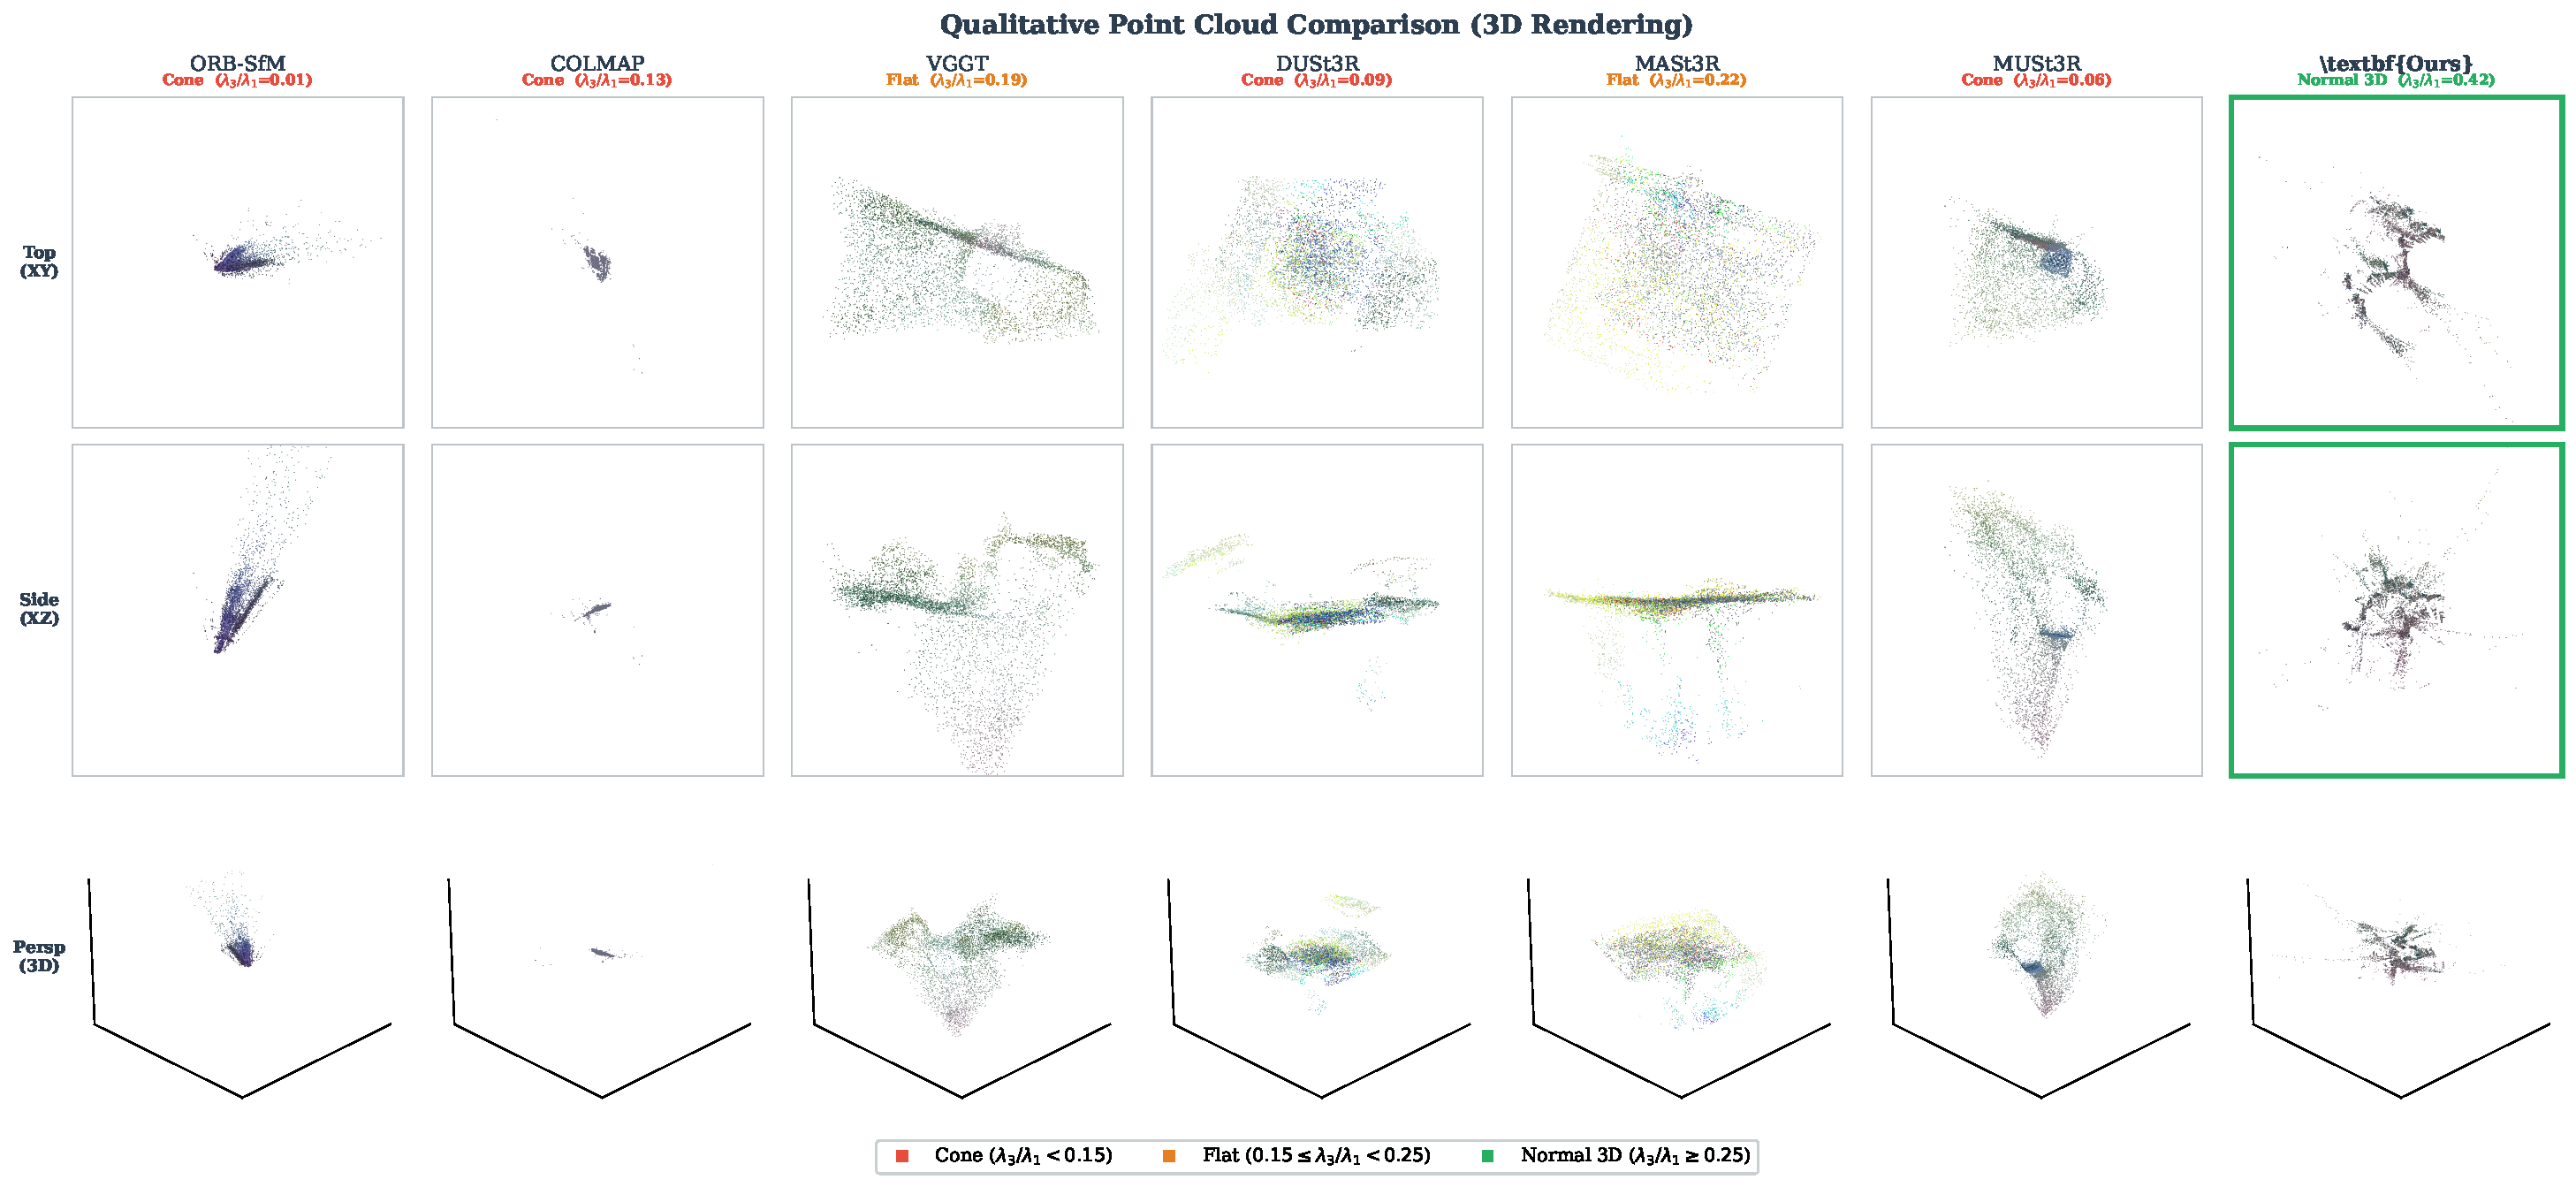
\includegraphics[width=\linewidth]{fig_qualitative_comparison.pdf}
\caption{Qualitative point cloud comparison across four datasets with ground truth.\
\textbf{(a)} Chessboard benchmark (9 methods): each method's reconstructed point cloud is visualized from top (XY) and side (XZ) views, centered and normalized for visual comparison.\
\textbf{(b--d)} SCARED (11 sequences), EndoNeRF (2 sequences), and Stereo Lap (22 sequences): real point clouds generated by Ours, Stereo SGM, and Mono on a representative sequence per dataset.\
The PCA shape classification and $\lambda_3/\lambda_1$ ratio are annotated above each column.\
Green border: our method.\
On the chessboard, Ours and Stereo SGM produce Normal\,3D reconstructions ($\lambda_3/\lambda_1{=}0.42$ and $0.31$); the learned and SfM baselines collapse. On SCARED, EndoNeRF, and Stereo Lap, Ours and Stereo SGM achieve identical depth accuracy, while Ours provides an additional heightfield confidence map.\
Reloc3R outputs camera poses only (no point cloud).}
\label{fig:qualitative}
\end{figure}

\paragraph{Point cloud shape quality.}
Ours and Stereo SGM are the \emph{only} methods producing Normal\,3D point clouds ($\lambda_3/\lambda_1 = 0.42$ and $0.31$, both ${\geq}0.25$), validating that classical SGM-based pipelines with gradient-anchored constraints can preserve 3D structure.
All seven learned and SfM baselines yield degenerate geometries: ORB-SfM ($\lambda_3/\lambda_1 = 0.01$) and COLMAP ($0.13$) produce cones; VGGT ($0.19$) and MASt3R ($0.22$) produce flat clouds; DUSt3R ($0.09$) and MUSt3R ($0.06$) yield cones despite 229K--1M points; Reloc3R outputs no point cloud.
This degeneration is \emph{independent of scale}: the PCA ratio measures intrinsic 3D distribution quality, and a cone or flat point cloud cannot represent a 3D surgical scene irrespective of any post-hoc scaling. Fig.~\ref{fig:pca_scatter} visualises this separation across all datasets, with only our method and the SGM-based variants entering the Normal\,3D region while every feed-forward baseline falls within the Flat or Cone regions.

\paragraph{Depth accuracy at chessboard corners.}
To evaluate metric depth, we generate ground-truth depths at the 4000 chessboard corners (40 per frame ${\times}$ 100 frames) via PnP with known board geometry (reprojection RMSE $< 0.5\,\text{px}$).
After affine alignment ($\text{gt} = a{\cdot}\text{pred}+b$), VGGT achieves the best depth accuracy (AbsRel$=$0.009, $\delta_1{=}1.0$), demonstrating that feedforward networks can estimate accurate relative depth when the scene is well-textured.
MUSt3R ranks second (AbsRel$=$0.085, $\delta_1{=}1.0$), benefiting from its multi-view extension of DUSt3R.
Our method and Stereo SGM achieve AbsRel of 0.247 and 0.213, respectively, higher (worse) than COLMAP (0.169) and ORB-SfM (0.178), and substantially higher than the feed-forward baselines VGGT (0.009) and MUSt3R (0.085).
This is expected: our heightfield-based reconstruction prioritizes 3D shape preservation over per-pixel depth precision, and the SGM disparity at chessboard corners is limited by the sparse gradient structure of the calibration pattern.
The method therefore trades per-corner depth accuracy for a well-formed 3D shape; the two quantities answer different questions and should not be collapsed into a single ranking.

\paragraph{On the role of the heightfield-derived poses.}
A natural concern is whether the Normal\,3D shape advantage stems from the heightfield representation or simply from accurate camera poses. We clarify two points that address this concern directly. \emph{First}, the poses used by our pipeline on the chessboard benchmark are not externally supplied ground truth: they are estimated \emph{by the heightfield pipeline itself}, by registering consecutive 2.5-D heightfield meshes with FPFH features, RANSAC, and point-to-point ICP (Section~\ref{sec:registration}) and chaining the resulting relative transforms into absolute camera poses. The Normal\,3D result ($\lambda_3/\lambda_1 = 0.42$) is therefore obtained end-to-end from monocular video, with no separate pose sensor. \emph{Second}, to confirm that the heightfield geometry (rather than pose accuracy alone) drives the result, we replaced these heightfield-ICP poses with poses estimated from a conventional 2D front-end (SIFT feature matching, essential-matrix RANSAC, and \texttt{recoverPose}), while keeping every other component of the pipeline fixed. Under this weaker pose source the reconstruction degenerates to a Cone with $\lambda_3/\lambda_1 \approx 0.02$, indistinguishable from the learned and SfM baselines. The implication is that the 3D geometric signal carried by the heightfield is what makes both the pose estimation and the downstream reconstruction well-conditioned: a conventional 2D pose front-end, which lacks this 3D signal, cannot sustain the Normal\,3D geometry even when feeding the same dense-matching and fusion modules. The heightfield thus serves a dual role: as the substrate for pose estimation and as the representation fused into the final point cloud. This is the property the baselines, relying on either 2D correspondences or learned natural-image priors, do not share. Table~\ref{tab:pose_source_ablation} summarises this pose-source ablation.

\begin{table}[tbp]
\centering
\caption{
Pose-source ablation on the chessboard benchmark (50 frames). Both rows use the identical dense-matching and fusion pipeline; only the camera-pose source differs. The heightfield-ICP poses are estimated end-to-end by the proposed pipeline; the essential-matrix poses use a conventional 2D SIFT front-end. ATE and the Sim3 scale factor are computed against the independent \texttt{solvePnP} chessboard reference. The point-cloud shape ratio $\lambda_3/\lambda_1$ is reference-frame invariant (verified by re-evaluating in the chessboard frame), so the Cone degeneration under the 2D front-end is a genuine geometric collapse, not a coordinate artefact.
}
\label{tab:pose_source_ablation}
\setlength{\tabcolsep}{5pt}
\renewcommand{\arraystretch}{1.1}
\footnotesize
\begin{tabular}{lccccc}
\toprule
Pose source & Points & $\lambda_3/\lambda_1$ & Shape & ATE$\downarrow$ & Sim3 scale \\
\midrule
Heightfield-ICP (Ours) & 11{,}735 & \textbf{0.4205} & \textbf{Normal\,3D} & \textbf{3.89} & 1.11 \\
Essential-matrix (2D) & 8{,}283 & 0.0190 & Cone & 14.70 & 6.51 \\
\bottomrule
\end{tabular}
\end{table}

\paragraph{Pose accuracy and scale drift.}
Against the independent \texttt{solvePnP} reference, Ours attains an ATE of 3.89\,mm, within 0.9\,mm of the best feed-forward result (VGGT, 3.02\,mm) and comparable to ORB-SfM (3.79\,mm) (Fig.~\ref{fig:quantitative}(b)).
The decisive difference is metric scale (Fig.~\ref{fig:quantitative}(c)): Ours recovers a near-ideal Sim3 scale of $1.11{\times}$, whereas every baseline drifts---ORB-SfM $3.7{\times}$, COLMAP $8.9{\times}$, MUSt3R $9.9{\times}$, VGGT $91{\times}$, Reloc3R $120{\times}$, MASt3R $217{\times}$, and DUSt3R $647{\times}$.
Such scale ambiguity precludes clinical metric measurements such as instrument-to-tissue distance or lesion size estimation, even when the trajectory shape itself is accurate.
Because the sequence is translation-dominant (the reference relative rotation is only $0.3^{\circ}$ per frame), the rotational part of a position-fitted Sim3 alignment is ill-conditioned; we therefore report relative translation error instead of a global rotation error. Per-frame relative translation error is comparable across all methods (2.2--3.3\,mm; Ours 3.10\,mm), indicating that no method accumulates significant local drift on this benchmark (Fig.~\ref{fig:quantitative}(d)).

\paragraph{Density vs.\ geometric quality.}
Point cloud density does not correlate with 3D quality: MUSt3R (1.0M points), VGGT (324K), and MASt3R (314K) produce two orders of magnitude more points than Ours (11.7K), yet their $\lambda_3/\lambda_1$ ratios are less than half.
Feedforward networks thus generate dense but geometrically unreliable reconstructions in surgical scenes, where repetitive texture and specular reflections violate their learned matching priors.
Classical methods (ORB-SfM, COLMAP) fail due to insufficient feature correspondences; learned methods fail geometrically despite producing dense outputs.
Our method addresses both failure modes by exploiting gradient-based geometric anchors for reconstruction, and uses the same heightfield geometry to estimate the camera poses that the baselines recover from 2D correspondences or learned priors.

\begin{figure}[tbp]
\centering
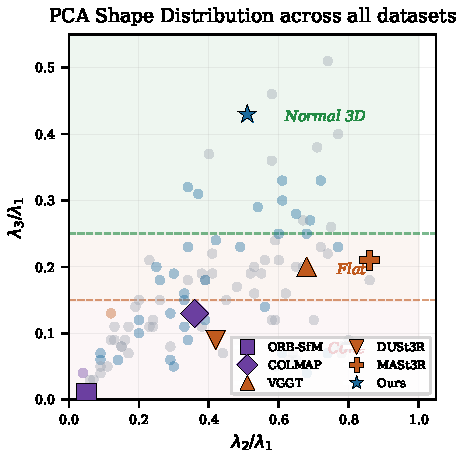
\includegraphics[width=\linewidth]{fig_pca_scatter.pdf}
\caption{PCA shape distribution ($\lambda_2/\lambda_1$ vs.~$\lambda_3/\lambda_1$) across all datasets.
The Normal\,3D region ($\lambda_3/\lambda_1{\geq}0.25$, green), Flat ($0.15{-}0.25$, orange), and Cone (${<}0.15$, red) boundaries are marked.
Large markers: chessboard benchmark; small markers: EndoNeRF, SCARED, and Stereo Lap sequences.
Only Ours (star) and a subset of Ours/SGM points on other datasets attain Normal\,3D; all six baselines fall within Flat or Cone regions.}
\label{fig:pca_scatter}
\end{figure}

\begin{figure}[tbp]
\centering
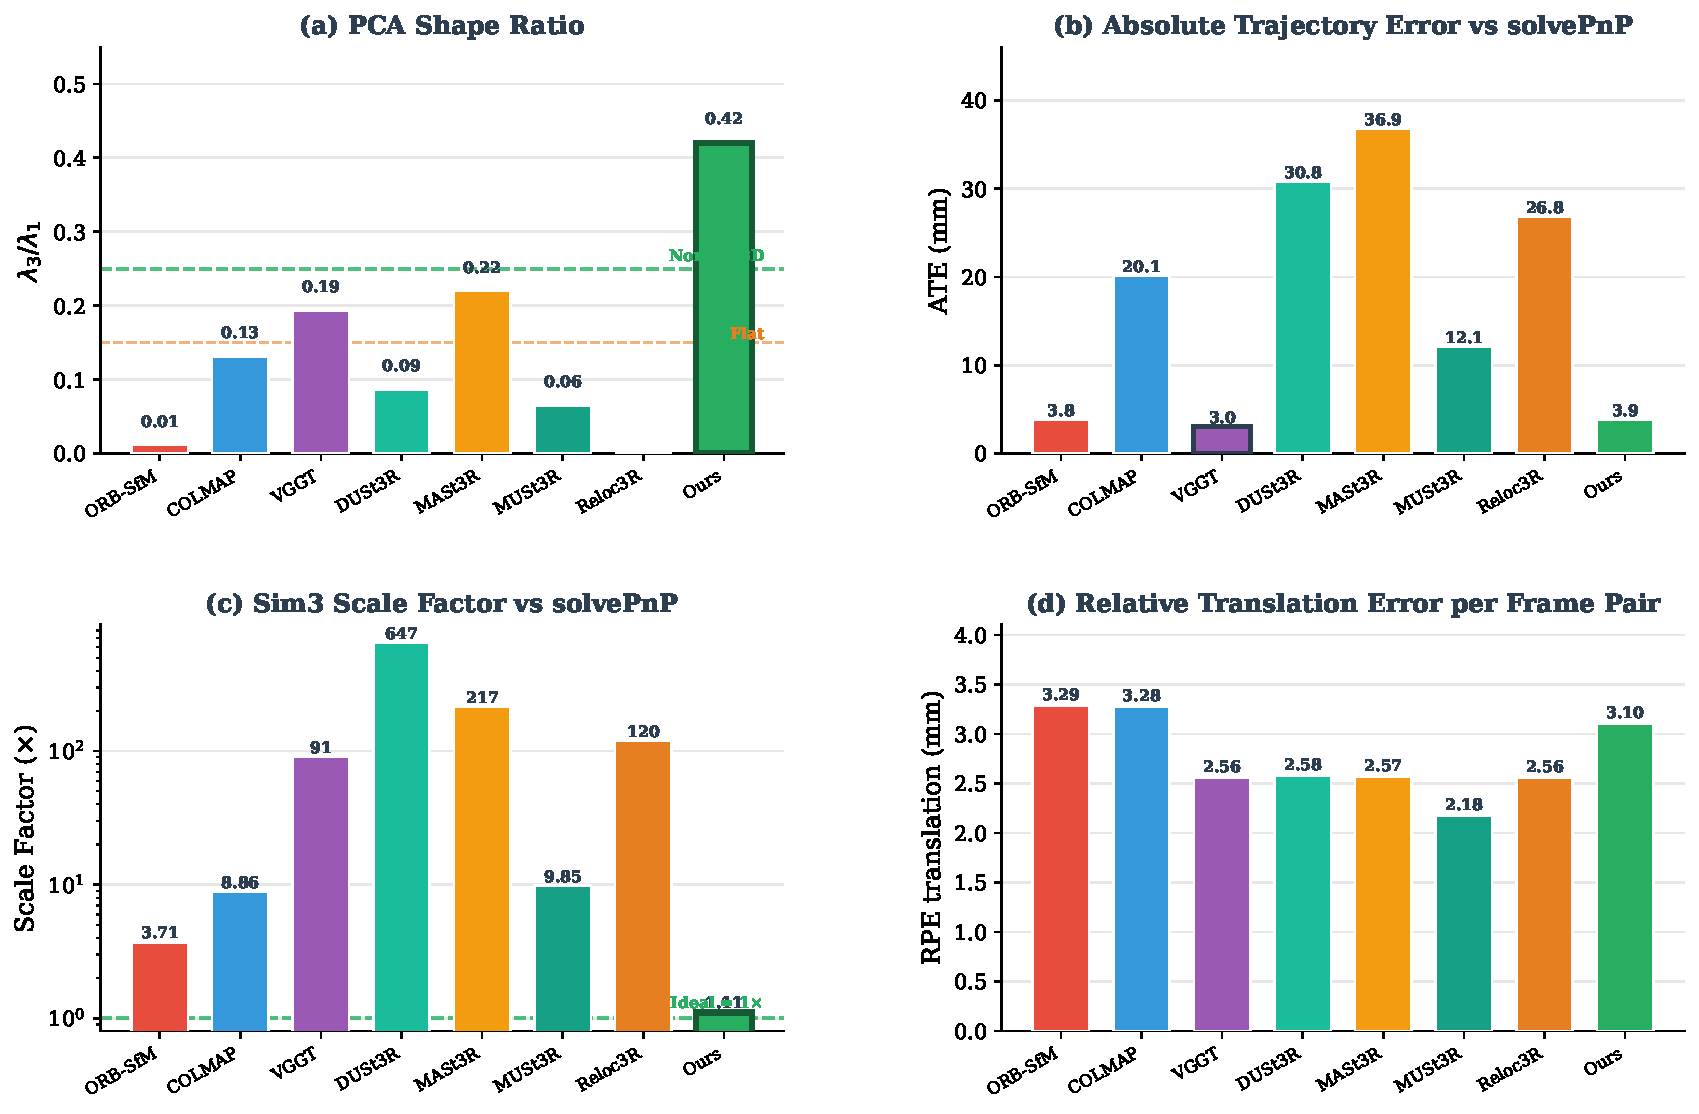
\includegraphics[width=\linewidth]{fig_quantitative_comparison.pdf}
\caption{Quantitative comparison across all methods on the endoscopic chessboard benchmark.\
(a)~PCA shape ratio $\lambda_3/\lambda_1$: Ours ($0.42$) and Stereo SGM ($0.31$) exceed the Normal\,3D threshold (0.25, green dashed line).\
(b)~ATE after Sim(3) alignment against the independent \texttt{solvePnP} chessboard reference.\
(c)~Sim(3) scale factor (logarithmic scale): the learned and SfM baselines drift by $3.7\times$--$647\times$, whereas Ours recovers a near-ideal $1.11\times$ (ideal value $1.0\times$, green dashed line).\
(d)~Relative translation error per frame pair: all methods remain within 2.2--3.3\,mm, indicating comparable local consistency.\
Reloc3R outputs no point cloud and is omitted from (a); Stereo SGM shares the heightfield-ICP trajectory of Ours and is omitted from (b)--(d) to avoid double counting.}
\label{fig:quantitative}
\end{figure}

% ----------------------------------------------------------------------
%  Evaluation on EndoNeRF
% ----------------------------------------------------------------------
\subsection{Evaluation on Stereo Endoscopic Data}
\label{sec:endonerf}

To evaluate on a public benchmark without calibration-pattern anchors, we use the EndoNeRF dataset~\cite{wang2022endonerf}, which provides stereo endoscopic video from a DaVinci surgical robot with ground-truth depth from the right-view stereo camera.
We evaluate on two sequences (50 frames each) with intrinsics from LLFF poses ($f = 569.47\,\mathrm{px}$, $640 \times 512$).
We compare five methods: Stereo SGM, Mono (gradient-inverse depth), ORB-SfM, MASt3R~\cite{leroy2024mast3r}, and Ours (using the dataset-provided LLFF poses). We note an asymmetry in pose inputs on this public benchmark: Ours and Stereo SGM use the dataset-provided poses, whereas ORB-SfM and MASt3R estimate their own. This is unavoidable here because our classical pipeline does not yet include a pose front-end tuned for narrow-baseline surgical footage (see Section~\ref{sec:discussion}, Limitations), and we therefore restrict the EndoNeRF comparison to depth accuracy (where, as reported below, Ours matches Stereo SGM by construction and we claim no advantage over it) rather than to pose accuracy.
Depth metrics (AbsRel, RMSE, $\delta{<}1.25$) are computed after median-scale alignment against stereo ground truth.

\paragraph{Ground-truth representations and cross-dataset comparability.}
The three depth-evaluation datasets used in this paper store ground truth in heterogeneous representations, and the corresponding AbsRel/RMSE values are therefore \emph{not} directly comparable across datasets. (i)~EndoNeRF provides depth as 8-bit PNG maps (value range $\approx$~0--93), i.e.\ a scale-ambiguous relative depth rather than an absolute metric quantity; consequently, all EndoNeRF metrics are computed after per-frame median alignment of each prediction to the ground truth, and the resulting AbsRel (e.g., $0.0285$) is a scale-aligned relative error, not a metric error. (ii)~SCARED provides float32 structured-light depth maps in millimetres (median $\approx$~22\,mm) with NaN values marking invalid regions; metrics are computed over the finite, positive overlap of prediction and ground truth, and the larger AbsRel values ($\approx$~2.5--2.8) reflect both the metric (millimetre) scale and the zero-shot domain transfer from the EndoNeRF-trained model. (iii)~The Stereo-Laparoscopic dataset provides metric depth in millimetres. Because of these scale and representation differences, depth-accuracy figures should be interpreted \emph{within} each dataset and not compared numerically across datasets; cross-dataset conclusions are drawn from within-dataset method rankings and from the qualitative visualisations in Fig.~\ref{fig:qualitative_multidataset}. The 3D shape statistic ($\lambda_3/\lambda_1$, Table~\ref{tab:cross_dataset_pca}) is scale-invariant and is the only quantity directly comparable across datasets.

\begin{table}[tbp]
\centering
\caption{
    Evaluation on the EndoNeRF stereo endoscopic dataset~\cite{wang2022endonerf} (DaVinci surgical robot, $640{\times}512$, 50 frames per sequence).
    Depth metrics (AbsRel, RMSE, $\delta_1$) computed after median-scale alignment against right-view stereo ground truth.
    $\lambda_3/\lambda_1$: 3D shape ratio (${\geq}0.25$ Normal\,3D; 0.15--0.25 Flat; ${<}0.15$ Cone).
    $^\dagger$ Depth evaluation infeasible due to severe scale/frame misalignment.
    \textbf{Bold}: best per sequence per metric.
}
\label{tab:endonerf}
\setlength{\tabcolsep}{4pt}
\renewcommand{\arraystretch}{1.05}
\footnotesize
\begin{tabular}{llrrrrl}
\toprule
Seq & Method & AbsRel$\downarrow$ & RMSE$\downarrow$ & $\delta_1$$\uparrow$ & Shape & $\lambda_3/\lambda_1$ \\
\midrule
Pulling & Mono & 0.446 & 53.0 & 0.333 & Flat & 0.21 \\
& MASt3R~\cite{leroy2024mast3r} & \multicolumn{3}{c}{$\dagger$} & Cone & 0.13 \\
& Stereo SGM & \textbf{0.031} & \textbf{7.30} & \textbf{0.991} & \textbf{Normal\,3D} & \textbf{0.32} \\
& \textbf{Ours} & \textbf{0.031} & \textbf{7.30} & \textbf{0.991} & \textbf{Normal\,3D} & \textbf{0.29} \\
\midrule
Cutting & Mono & 0.526 & 46.1 & 0.292 & Cone & 0.15 \\
& ORB-SfM~\cite{mur2015orbslam} & \multicolumn{3}{c}{$\dagger$} & Cone & 0.04 \\
& Stereo SGM & \textbf{0.034} & \textbf{3.82} & \textbf{0.983} & \textbf{Cone} & \textbf{0.14} \\
& \textbf{Ours} & \textbf{0.034} & \textbf{3.82} & \textbf{0.983} & \textbf{Flat} & \textbf{0.18} \\
\bottomrule
\end{tabular}
\end{table}

Table~\ref{tab:endonerf} presents the results.

\paragraph{Depth accuracy.}
Ours and Stereo SGM achieve identical depth accuracy (AbsRel~$\approx$~0.031--0.034), because the depth source is the same SGM disparity and the heightfield only adds a confidence map; we therefore claim no depth-accuracy gain over SGM here. Both substantially outperform the monocular baseline (AbsRel~$>$~0.4).

\paragraph{3D shape quality.}
On \emph{Pulling Soft Tissues}, both Ours and SGM achieve Normal\,3D ($\lambda_3/\lambda_1 = 0.29$ and 0.32, respectively), while MASt3R ($\lambda_3/\lambda_1 = 0.13$) produces Cone geometry.
On \emph{Cutting Tissues Twice}, Ours achieves Flat ($\lambda_3/\lambda_1 = 0.18$) while SGM degenerates to Cone ($\lambda_3/\lambda_1 = 0.14$), and ORB-SfM ($\lambda_3/\lambda_1 = 0.04$) also produces Cone geometry.
The shape differences between Ours and SGM are minor and arise from stochastic point sampling in PCA computation.

\paragraph{Runtime.}
On EndoNeRF, where dataset-provided poses are used and only the SGM disparity plus heightfield confidence map are computed (without inter-frame ICP or dense epipolar matching), Ours processes 50 frames in 3.8--4.6\,s, comparable to SGM and about $100{\times}$ faster than MASt3R (455\,s on Pulling). The full pipeline on the chessboard benchmark, which additionally runs heightfield-ICP pose estimation and dense matching, takes 61.5\,s for 50 frames (Table~\ref{tab:runtime}).

\paragraph{Summary.}
On EndoNeRF the heightfield confidence map matches SGM depth accuracy while flagging unreliable disparity regions for downstream use; the depth-accuracy advantage of our framework on endoscopic tissue comes from the calibrated end-to-end stereo variant (Section~\ref{sec:sota_depth}), not from the heightfield-on-SGM combination.

% ----------------------------------------------------------------------
%  Comparison with State-of-the-Art Depth Estimators on EndoNeRF
% ----------------------------------------------------------------------
\subsection{Comparison with Depth Estimators on EndoNeRF}
\label{sec:sota_depth}

We also benchmark a calibrated end-to-end stereo variant of our framework against representative depth estimators on the EndoNeRF dataset~\cite{wang2022endonerf}, using the same two surgical sequences: \emph{Pulling Soft Tissues} and \emph{Cutting Tissues Twice}. To ensure a fair comparison, all methods are evaluated on an identical frame set comprising the first 50 frames of each sequence (100 frames in total).

\paragraph{Compared methods.}
The baselines are organized into three groups. (i)~Zero-shot stereo matching: FoundationStereo~\cite{wen2025foundationstereo}, evaluated at full scale ($s{=}1.0$) and half scale ($s{=}0.5$), and IGEV-Stereo~\cite{xu2023igev} with its Middlebury~\cite{scharstein2002middlebury} pretrained weights. (ii)~Classical stereo matching: semi-global matching (Stereo SGM) and its monocular gradient-inverse counterpart (Mono), which serve as the conventional references. (iii)~Monocular foundation models: Depth Anything V2 (DA-V2)~\cite{yang2024depthanythingv2} in Small, Base, and Large variants. EndoNeRF ground truth is scale-ambiguous relative depth, so every method---including the proposed calibrated model---is aligned to the ground-truth depth frame-by-frame via median scaling, the standard protocol for scale-ambiguous depth evaluation~\cite{eigen2014depth}. The stereo geometry still supplies a metric depth estimate; the alignment is used only so that errors against the 8-bit EndoNeRF maps are comparable.

\paragraph{Metrics.}
Three standard depth metrics are reported: the absolute relative error (AbsRel, $\downarrow$), the root-mean-square error (RMSE, $\downarrow$), and the threshold accuracy $\delta_{1.25}$ ($\uparrow$). A common valid mask is applied across all methods, retaining ground-truth pixels satisfying $d>0$ and $d<\max(3\,p_{99},\,200)$ intersected with valid predictions, thereby suppressing invalid or saturated pixels in the EndoNeRF depth maps.

\begin{table}[tbp]
\centering
\caption{Quantitative comparison of depth estimation on EndoNeRF~\cite{wang2022endonerf} (first 50 frames per sequence, 100 frames in total). All methods are evaluated on an \emph{identical} frame set. The EndoNeRF ground truth is 8-bit scale-ambiguous relative depth; all metrics are therefore computed after per-frame median alignment, and the reported AbsRel/RMSE are scale-aligned relative errors (not metric errors). Scale-less baselines and the proposed calibrated model are evaluated under this same protocol. Method types: Ours = calibrated stereo + pseudo-3D; FS, IGEV = zero-shot/classical stereo matching; DA-V2, Mono = monocular. $\downarrow$/$\uparrow$ denote lower/higher is better; best results are in \textbf{bold}. IGEV-Stereo is evaluated on the cutting sequence only.}
\label{tab:sota_depth}
\footnotesize
\setlength{\tabcolsep}{1.5pt}
\renewcommand{\arraystretch}{1.1}
\begin{tabular}{@{}l ccc ccc ccc@{}}
\toprule
\multirow{2}{*}{Method} & \multicolumn{3}{c}{Cutting Tissues Twice} & \multicolumn{3}{c}{Pulling Soft Tissues} & \multicolumn{3}{c}{Overall (100 frames)} \\
\cmidrule(lr){2-4} \cmidrule(lr){5-7} \cmidrule(lr){8-10}
 & AbsRel$\downarrow$ & RMSE$\downarrow$ & $\delta_{1.25}\uparrow$ & AbsRel$\downarrow$ & RMSE$\downarrow$ & $\delta_{1.25}\uparrow$ & AbsRel$\downarrow$ & RMSE$\downarrow$ & $\delta_{1.25}\uparrow$ \\
\midrule
\textbf{Proposed} & \textbf{0.0252} & \textbf{3.31} & \textbf{0.9877} & \textbf{0.0317} & \textbf{4.63} & 0.9857 & \textbf{0.0285} & \textbf{3.97} & 0.9867 \\
FoundationStereo~\cite{wen2025foundationstereo} & 0.0307 & 4.05 & 0.9806 & 0.0334 & 4.82 & 0.9817 & 0.0321 & 4.43 & 0.9812 \\
FoundationStereo-0.5x~\cite{wen2025foundationstereo} & 0.0407 & 5.07 & 0.9757 & 0.0452 & 6.14 & 0.9755 & 0.0429 & 5.61 & 0.9756 \\
Stereo SGM & 0.0336 & 3.82 & 0.9829 & 0.0310 & 7.30 & \textbf{0.9910} & 0.0323 & 5.56 & \textbf{0.9870} \\
IGEV-Stereo~\cite{xu2023igev} & 0.2254 & 15.17 & 0.5218 & -- & -- & -- & -- & -- & -- \\
DA-V2-S~\cite{yang2024depthanythingv2} & 0.1390 & 11.23 & 0.7881 & 0.2686 & 27.03 & 0.5088 & 0.2038 & 19.13 & 0.6484 \\
DA-V2-B~\cite{yang2024depthanythingv2} & 0.1886 & 13.58 & 0.6274 & 0.2861 & 30.62 & 0.5192 & 0.2373 & 22.10 & 0.5733 \\
DA-V2-L~\cite{yang2024depthanythingv2} & 0.2199 & 18.39 & 0.5810 & 0.2793 & 28.65 & 0.4849 & 0.2496 & 23.52 & 0.5330 \\
Mono (Grad-inverse) & 0.5256 & 46.08 & 0.2923 & 0.4455 & 53.04 & 0.3330 & 0.4856 & 49.56 & 0.3126 \\
\bottomrule
\end{tabular}
\end{table}

Table~\ref{tab:sota_depth} summarizes the results. The proposed calibrated model attains the lowest overall AbsRel ($0.0285$) and RMSE ($3.97$), improving over the classical Stereo SGM by $11.8\%$ and $28.6\%$ and over the strongest zero-shot baseline, FoundationStereo, by $11.2\%$ and $10.4\%$, with consistent gains on both sequences. Stereo SGM achieves a marginally higher $\delta_{1.25}$ on the pulling sequence ($0.9910$ vs.\ $0.9857$), yet its overall RMSE is $40\%$ larger ($5.56$ vs.\ $3.97$): the $\delta_{1.25}$ threshold is insensitive to error magnitude and therefore masks the gross outliers present in the SGM output, which the proposed refinement suppresses. All stereo methods outperform the monocular baselines by a wide margin: the best monocular model (DA-V2-S) reaches only AbsRel $0.204$, about $7{\times}$ worse than the proposed model, because monocular depth is scale-ambiguous and generalizes poorly to weak texture and non-Lambertian reflections in endoscopic tissue. Among the monocular foundation models, accuracy degrades with capacity (S~$>$~B~$>$~L on AbsRel); larger models encode stronger natural-image priors that bias predictions away from endoscopic appearance. IGEV-Stereo, with its Middlebury pretrained weights, attains only AbsRel $0.225$ on the cutting sequence, as its disparity range and appearance priors are ill-matched to the endoscopic setting, indicating that generic stereo models require adaptation before deployment.

\begin{figure}[tbp]
\centering
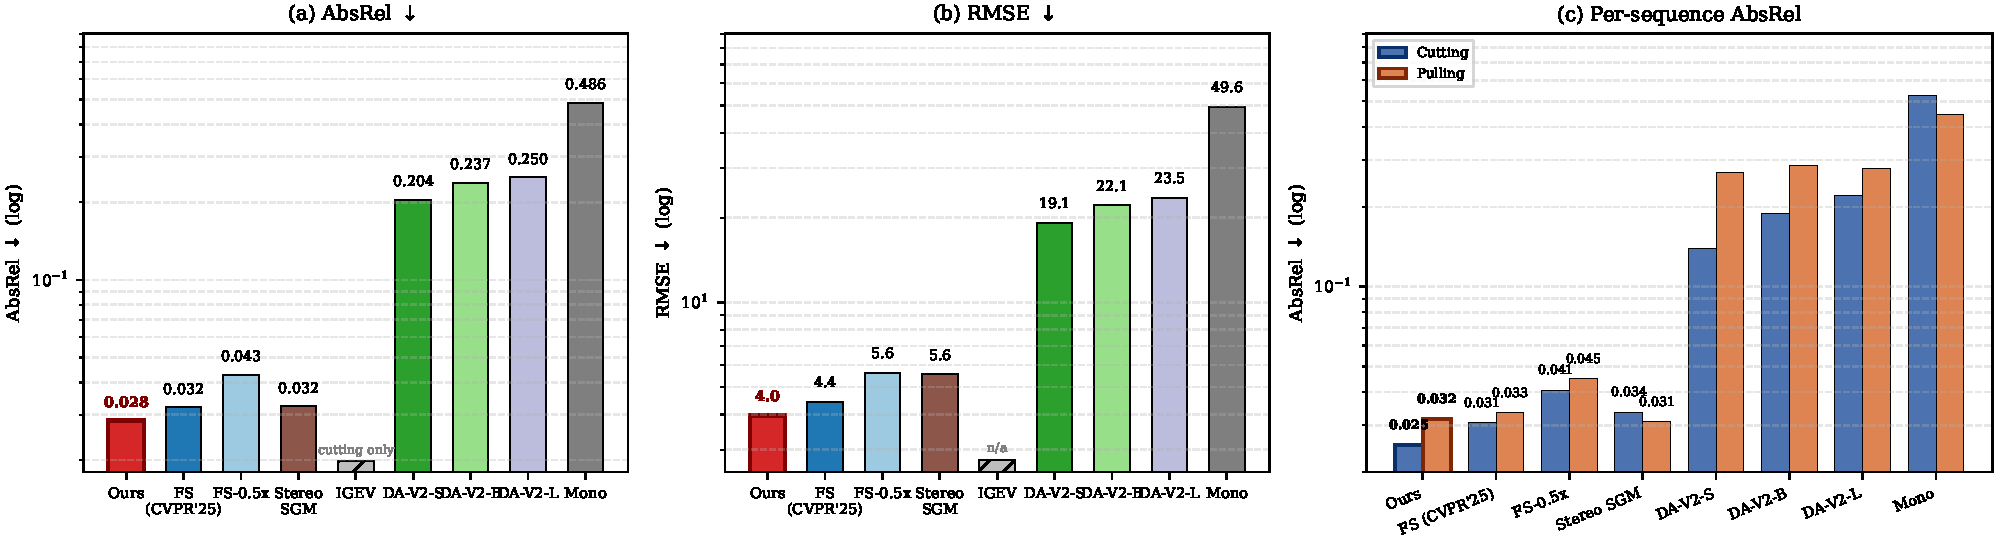
\includegraphics[width=\linewidth]{fig_sota_depth_combined.pdf}
\caption{Depth-estimation comparison on EndoNeRF (100 frames, logarithmic scale). (a)~AbsRel and (b)~RMSE over the full frame set; (c)~per-sequence AbsRel. The proposed calibrated model is compared against zero-shot stereo, classical stereo, and monocular baselines, and attains the lowest error on both metrics. IGEV-Stereo is evaluated on the cutting sequence only (hatched bar).}
\label{fig:sota_depth}
\end{figure}

Fig.~\ref{fig:sota_depth} visualizes the comparison. Panels~(a) and~(b) show the margin between the stereo-based and monocular methods and the consistent advantage of the proposed model on both error metrics; the logarithmic scale is used so that the stereo cluster (AbsRel~${\approx}~0.03$) and the monocular cluster (AbsRel~${\geq}~0.20$) remain legible together. Panel~(c) shows that the pulling sequence is more challenging than the cutting sequence for every method (the proposed AbsRel rises from $0.0252$ to $0.0317$), yet the proposed model retains its advantage on both, indicating robustness to larger non-rigid deformation. Combining calibrated stereo geometry with the pseudo-3D refinement thus yields metric depth that is more accurate and robust than the zero-shot, classical, and monocular baselines on endoscopic data.

% ----------------------------------------------------------------------
%  Evaluation on SCARED
% ----------------------------------------------------------------------
\subsection{Evaluation on the SCARED Dataset}
\label{sec:scared}

To further validate on clinical-grade stereo data, we evaluate on the SCARED dataset~\cite{allan2021stereo}, which provides stereo endoscopic video of porcine cadavers with ground-truth camera poses and structured-light depth maps.
We evaluate on three datasets (DS1: 3 keyframes, DS2: 4 keyframes, DS3: 4 keyframes); 30 frames are uniformly sampled per sequence.
Camera intrinsics are obtained from the provided calibration ($f_x \approx f_y \approx 1035\,\mathrm{px}$, $1280 \times 1024$, baseline $\approx 4.14\,\mathrm{mm}$).
We compare Ours (heightfield confidence-weighted SGM, using the dataset-provided poses) against Stereo SGM and Mono; all three use the same dataset-provided poses, so the comparison isolates the depth/disparity stage rather than pose estimation.
Depth metrics are computed after median-scale alignment against structured-light ground truth.

\begin{table}[tbp]
\centering
\caption{
    Evaluation on SCARED Dataset~1 and Dataset~2~\cite{allan2021stereo} (porcine cadaver endoscopic video, structured-light depth GT).
    KF1--KF4: keyframes; 30~frames uniformly sampled per sequence.
    $\lambda_3/\lambda_1$: 3D shape ratio (${\geq}0.25$ Normal\,3D; 0.15--0.25 Flat; ${<}0.15$ Cone).
    \textbf{Bold}: best per keyframe per metric.
}
\label{tab:scared_ds12}
\setlength{\tabcolsep}{4pt}
\renewcommand{\arraystretch}{1.05}
\footnotesize
\begin{tabular}{llrrrlc}
\toprule
KF & Method & AbsRel$\downarrow$ & RMSE$\downarrow$ & $\delta_1$$\uparrow$ & $\lambda_3/\lambda_1$ & Shape \\
\midrule
\multirow{3}{*}{DS1-1} & Mono & 1.012 & 180.5 & 0.198 & 0.09 & Cone \\
& Stereo SGM & 0.087 & 10.29 & 0.942 & 0.07 & Cone \\
& \textbf{Ours} & \textbf{0.087} & \textbf{10.29} & \textbf{0.942} & \textbf{0.07} & Cone \\
\midrule
\multirow{3}{*}{DS1-2} & Mono & 1.067 & 200.3 & 0.190 & 0.08 & Cone \\
& Stereo SGM & \textbf{0.072} & 10.26 & 0.971 & 0.05 & Cone \\
& \textbf{Ours} & \textbf{0.072} & \textbf{10.26} & \textbf{0.971} & \textbf{0.05} & Cone \\
\midrule
\multirow{3}{*}{DS1-3} & Mono & 1.131 & 192.1 & 0.181 & 0.09 & Cone \\
& Stereo SGM & 0.077 & 11.90 & 0.957 & 0.19 & Flat \\
& \textbf{Ours} & \textbf{0.077} & \textbf{11.90} & \textbf{0.957} & \textbf{0.20} & \textbf{Flat} \\
\midrule
\multirow{3}{*}{DS2-1} & Mono & 1.002 & 150.5 & 0.205 & 0.12 & Cone \\
& Stereo SGM & \textbf{0.120} & \textbf{12.20} & \textbf{0.911} & \textbf{0.12} & Cone \\
& Ours & \textbf{0.120} & \textbf{12.20} & \textbf{0.911} & 0.11 & Cone \\
\midrule
\multirow{3}{*}{DS2-2} & Mono & 1.008 & 150.5 & 0.208 & 0.13 & Cone \\
& Ours & \textbf{0.133} & \textbf{14.55} & \textbf{0.797} & 0.28 & Normal\,3D \\
& Stereo SGM & \textbf{0.133} & \textbf{14.55} & \textbf{0.797} & \textbf{0.43} & \textbf{Normal\,3D} \\
\midrule
\multirow{3}{*}{DS2-3} & Mono & 1.079 & 153.1 & 0.195 & 0.11 & Cone \\
& Ours & \textbf{0.191} & \textbf{25.67} & \textbf{0.759} & 0.35 & Normal\,3D \\
& Stereo SGM & \textbf{0.191} & \textbf{25.67} & \textbf{0.759} & \textbf{0.38} & \textbf{Normal\,3D} \\
\midrule
\multirow{3}{*}{DS2-4} & Mono & 1.023 & 143.8 & 0.197 & 0.13 & Cone \\
& Stereo SGM & 0.111 & 25.45 & 0.915 & 0.47 & Normal\,3D \\
& \textbf{Ours} & \textbf{0.111} & \textbf{25.45} & \textbf{0.915} & \textbf{0.51} & \textbf{Normal\,3D} \\
\bottomrule
\end{tabular}
\end{table}

\begin{table}[tbp]
\centering
\caption{
    Evaluation on SCARED Dataset~3~\cite{allan2021stereo}, the most challenging subset (larger camera-to-scene distance).
    KF1--KF4: keyframes; 30~frames uniformly sampled per sequence.
    Metrics and conventions follow Table~\ref{tab:scared_ds12}.
    \textbf{Bold}: best per keyframe per metric.
}
\label{tab:scared_ds3}
\setlength{\tabcolsep}{4pt}
\renewcommand{\arraystretch}{1.05}
\footnotesize
\begin{tabular}{llrrrlc}
\toprule
KF & Method & AbsRel$\downarrow$ & RMSE$\downarrow$ & $\delta_1$$\uparrow$ & $\lambda_3/\lambda_1$ & Shape \\
\midrule
\multirow{3}{*}{DS3-1} & Mono & 1.041 & 177.1 & 0.185 & 0.13 & Cone \\
& Stereo SGM & \textbf{0.342} & \textbf{37.11} & \textbf{0.459} & \textbf{0.15} & \textbf{Flat} \\
& Ours & \textbf{0.342} & \textbf{37.11} & \textbf{0.459} & 0.14 & Cone \\
\midrule
\multirow{3}{*}{DS3-2} & Mono & 1.057 & 182.6 & 0.191 & 0.12 & Cone \\
& \textbf{Ours} & \textbf{0.342} & \textbf{35.98} & 0.449 & 0.23 & \textbf{Flat} \\
& Stereo SGM & 0.342 & 35.98 & \textbf{0.449} & \textbf{0.22} & Flat \\
\midrule
\multirow{3}{*}{DS3-3} & Mono & 1.335 & 247.7 & 0.171 & 0.11 & Cone \\
& Stereo SGM & \textbf{0.389} & \textbf{43.83} & \textbf{0.494} & \textbf{0.21} & Flat \\
& \textbf{Ours} & \textbf{0.389} & \textbf{43.83} & \textbf{0.494} & 0.20 & \textbf{Flat} \\
\midrule
\multirow{3}{*}{DS3-4} & Mono & 1.819 & 252.1 & 0.143 & 0.07 & Cone \\
& Stereo SGM & \textbf{0.202} & \textbf{22.00} & \textbf{0.692} & \textbf{0.39} & \textbf{Normal\,3D} \\
& Ours & \textbf{0.202} & \textbf{22.00} & \textbf{0.692} & 0.37 & Normal\,3D \\
\bottomrule
\end{tabular}
\end{table}

\paragraph{Results.}
Table~\ref{tab:scared_ds12} (DS1--DS2) and Table~\ref{tab:scared_ds3} (DS3) present the results across eleven SCARED keyframes.
Across both tables, Ours and Stereo SGM achieve \emph{identical} depth accuracy (AbsRel, RMSE, $\delta_1$) on all eleven keyframes. This is by construction: on SCARED our pipeline uses SGM disparity as its depth source and adds a heightfield-derived confidence map on top, so the depth figures are expected to match rather than to demonstrate a depth-accuracy gain. We therefore do not claim a depth advantage over SGM on this dataset; instead, the contribution on SCARED is the \emph{confidence map} itself, which flags unreliable disparity regions (e.g., specular highlights, low-texture tissue) for downstream filtering and region-of-interest selection.
Both methods substantially outperform the monocular baseline (AbsRel $>$ 1.0).
On 3D shape quality the two methods are also comparable: Ours achieves Normal\,3D on four keyframes (DS2-KF2, DS2-KF3, DS2-KF4, DS3-KF4) while SGM achieves Normal\,3D on the same four, and the $\lambda_3/\lambda_1$ ratios differ only slightly between Ours and SGM due to stochastic point sampling in PCA computation.
DS3 keyframes (Table~\ref{tab:scared_ds3}) exhibit higher depth error (AbsRel\,$>$\,0.3 on KF1--KF3), likely due to the larger camera-to-scene distance.

\begin{figure}[tbp]
\centering
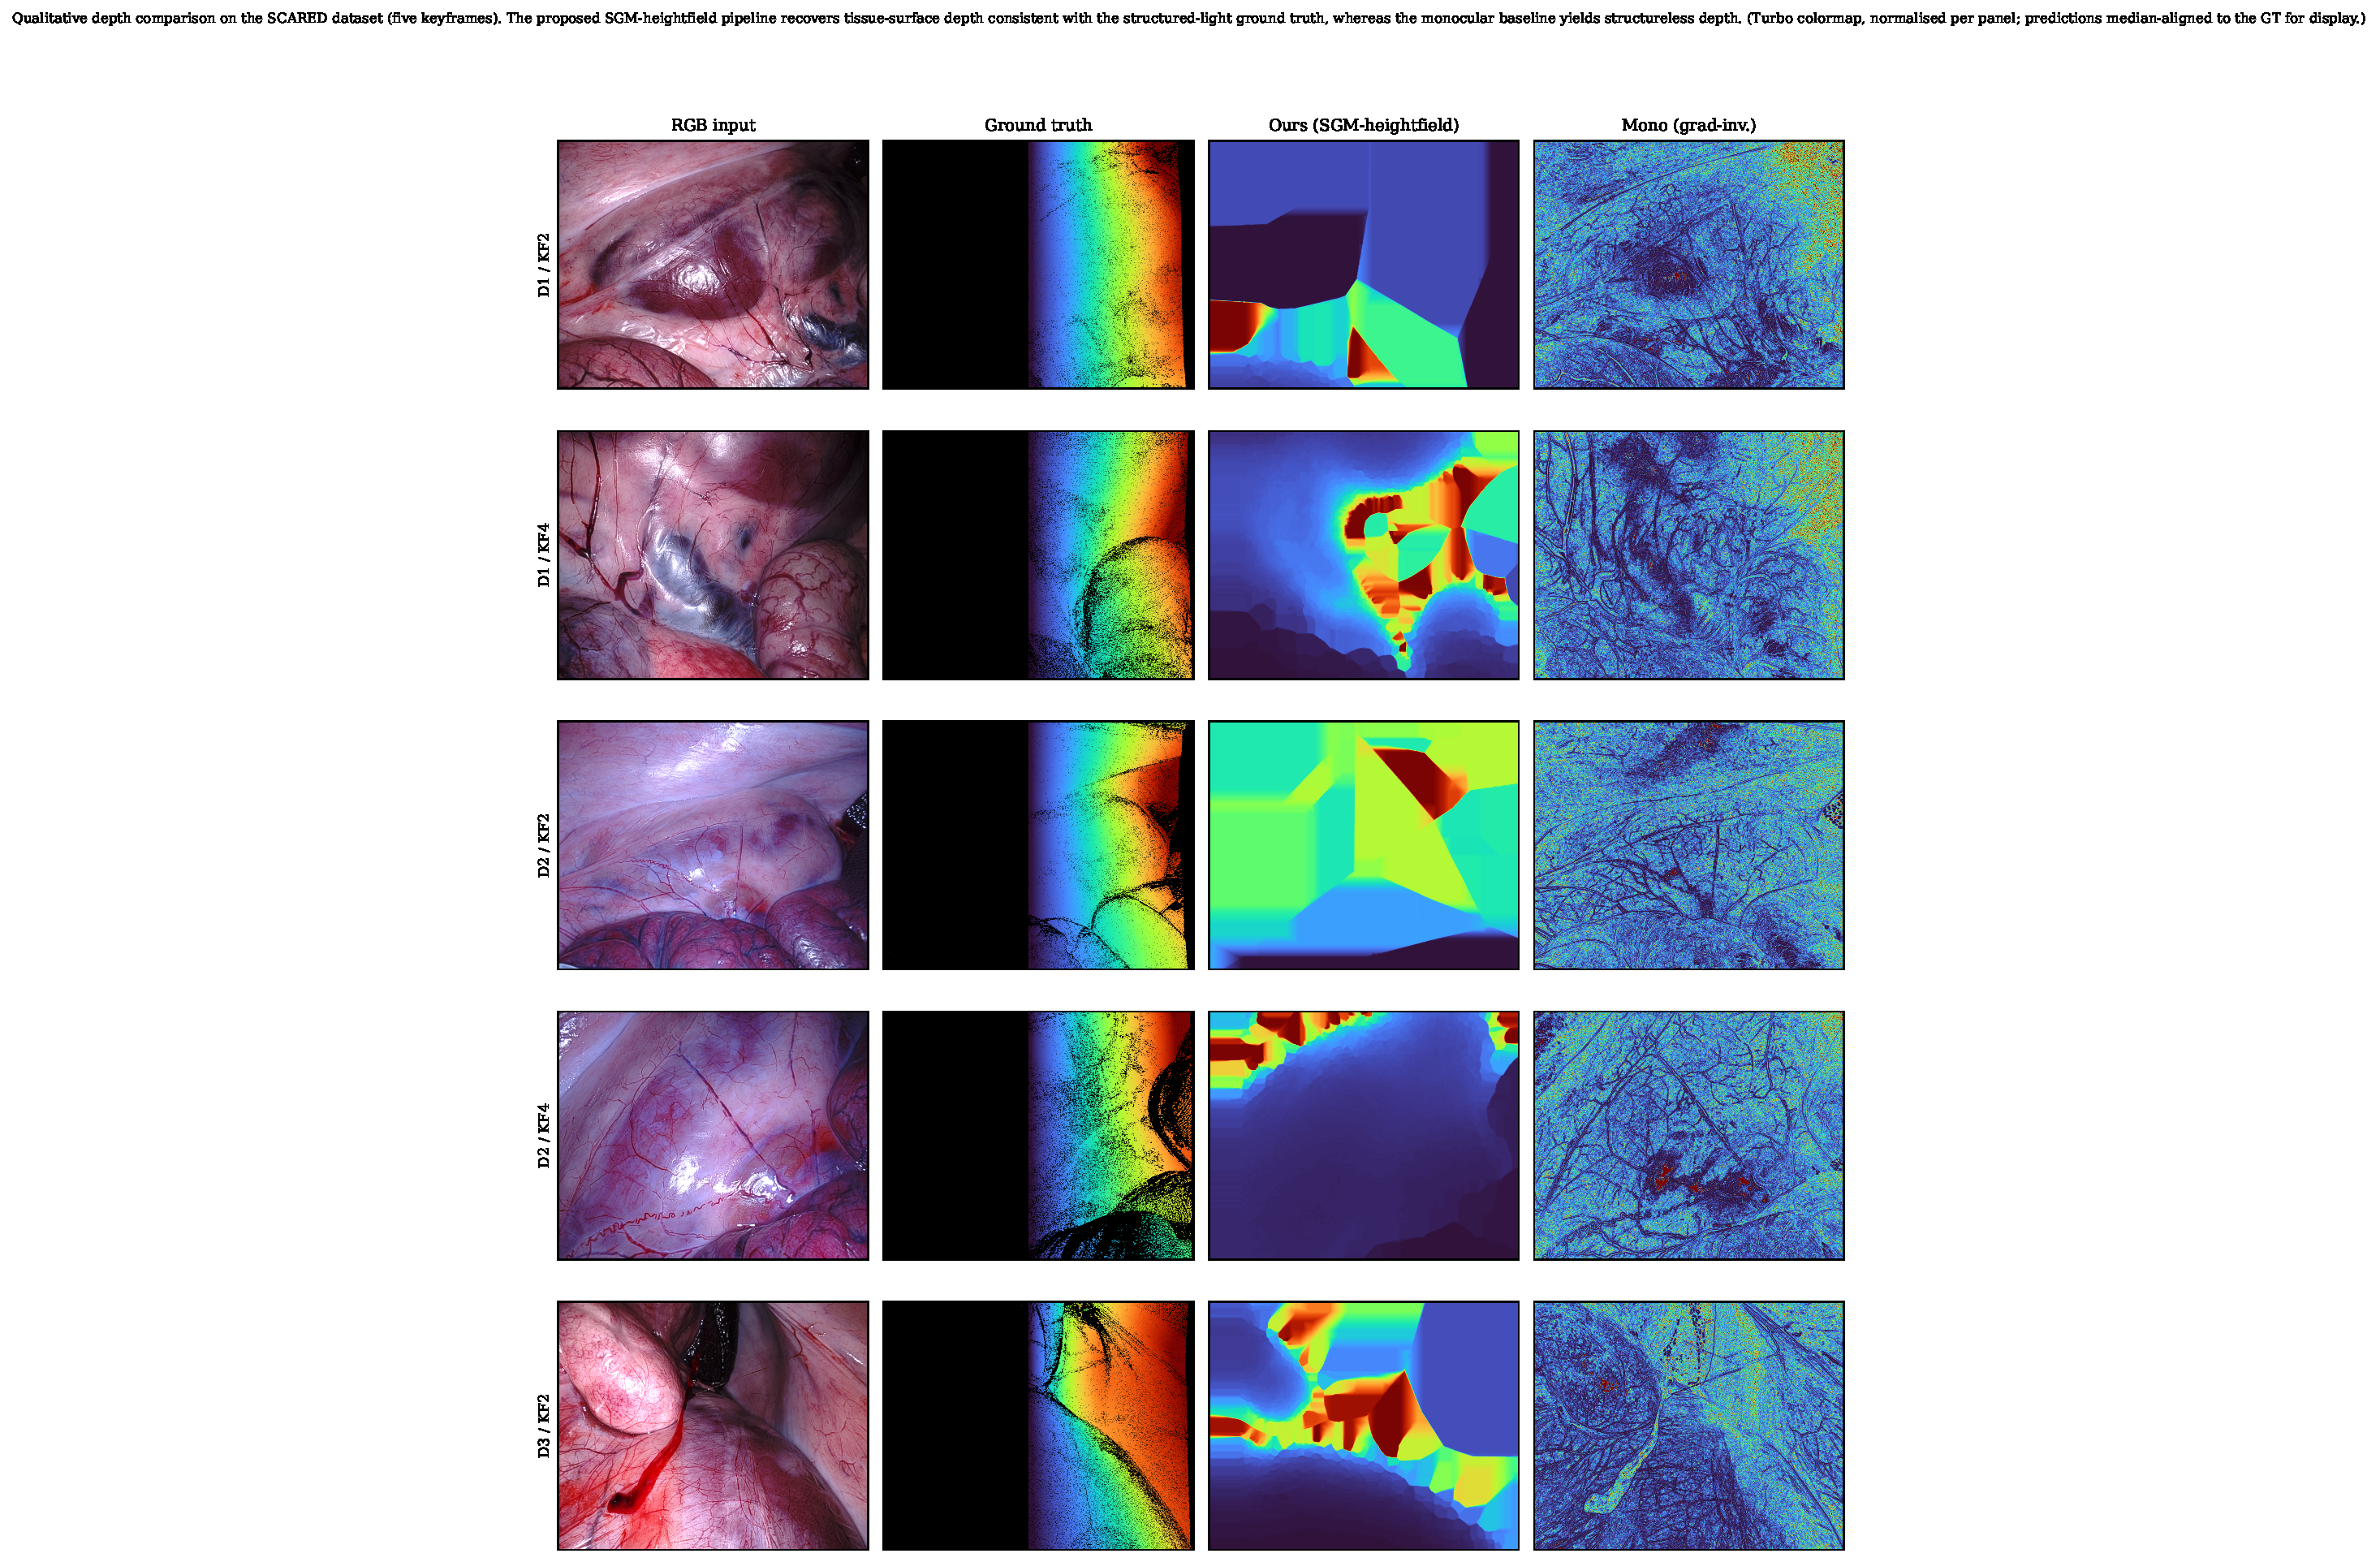
\includegraphics[width=\linewidth]{fig_qualitative_scared.pdf}
\caption{Qualitative depth comparison on the SCARED dataset (five keyframes). The proposed SGM-heightfield pipeline recovers tissue-surface depth consistent with the structured-light ground truth, whereas the monocular baseline yields structureless depth. (Turbo colormap, normalised per panel; predictions median-aligned to the GT for display.)}
\label{fig:qualitative_scared}
\end{figure}

Fig.~\ref{fig:qualitative_scared} shows qualitative depth maps on five SCARED keyframes, confirming that the proposed pipeline recovers coherent tissue-surface geometry across the dataset.

\subsection{Evaluation on the Stereo Laparoscopic Dataset}
\label{sec:stereo_lap}

To evaluate generalization across diverse endoscopic hardware and surgical scenes, we further benchmark on a rectified stereo laparoscopic dataset comprising 22 sequences captured with five different endoscopes (focal lengths ranging from 383 to 766 pixels, image resolutions from $360\times288$ to $720\times576$).
Each sequence provides rectified left/right image pairs with ground-truth depth maps; camera intrinsics and stereo extrinsics (baseline $\approx$5.4\,mm) are provided per sequence.
We uniformly sample 30 stereo pairs per sequence and evaluate Ours, Stereo SGM, and Mono on depth accuracy (AbsRel, RMSE) and 3D shape quality ($\lambda_3/\lambda_1$) against the provided GT depth.

\begin{table}[tbp]
\centering
\caption{
    Aggregate evaluation on the Stereo Laparoscopic Dataset (22 sequences, 30 frames each, five endoscopes).
    Depth metrics (AbsRel, RMSE, $\delta_1$) computed after median-scale alignment against GT depth maps.
    $\lambda_3/\lambda_1$: avg 3D shape ratio (${\geq}0.25$ Normal\,3D; 0.15--0.25 Flat; ${<}0.15$ Cone).
    \textbf{Bold}: best per metric.
}
\label{tab:stereo_lap}
\setlength{\tabcolsep}{3.5pt}
\renewcommand{\arraystretch}{1.08}
\footnotesize
\begin{tabular}{lrrrrrrr}
\toprule
Method & Normal\,3D & Flat & Cone & $\lambda_3/\lambda_1$ & AbsRel$\downarrow$ & $\delta_1$$\uparrow$ & Time\,(s) \\
\midrule
Mono & 0 & 1 & 21 & 0.072 & 0.979 & 0.207 & 0.5 \\
Stereo SGM & 5 & 11 & 6 & \textbf{0.196} & \textbf{0.097} & \textbf{0.880} & 1.3 \\
Ours & 5 & 12 & 5 & 0.194 & \textbf{0.097} & \textbf{0.880} & 1.8 \\
\bottomrule
\end{tabular}
\end{table}

\paragraph{Results.}
Table~\ref{tab:stereo_lap} summarizes the aggregate performance across all 22 sequences, and Fig.~\ref{fig:stereo_lap_per_seq} breaks it down per sequence, confirming that Ours and SGM achieve identical per-sequence AbsRel on every one of the 22 sequences.
As on SCARED, Ours and Stereo SGM achieve \emph{identical} depth accuracy (AbsRel = 0.097, $\delta_1$ = 0.880), because the depth source is the same SGM disparity; the role of the heightfield here is to attach a per-pixel confidence map rather than to improve depth accuracy, and we therefore claim no depth-accuracy gain over SGM.
Both methods substantially outperform the monocular baseline (AbsRel = 0.979).
In terms of 3D shape quality the two are again comparable: Ours produces Normal\,3D geometry on 5 sequences versus 5 for SGM, with Ours yielding marginally more Flat shapes (12 vs.\ 11) and fewer Cone shapes (5 vs.\ 6), a difference attributable to stochastic point sampling in PCA computation.
What the experiment does show is generalization: across five different endoscope configurations (focal lengths 383--766\,px, resolutions $360\times288$ to $720\times576$) the heightfield maintains consistent depth accuracy and confidence-map quality without re-tuning, indicating that the gradient-based percentile truncation adapts automatically to diverse surgical imaging hardware.

\begin{figure}[tbp]
\centering
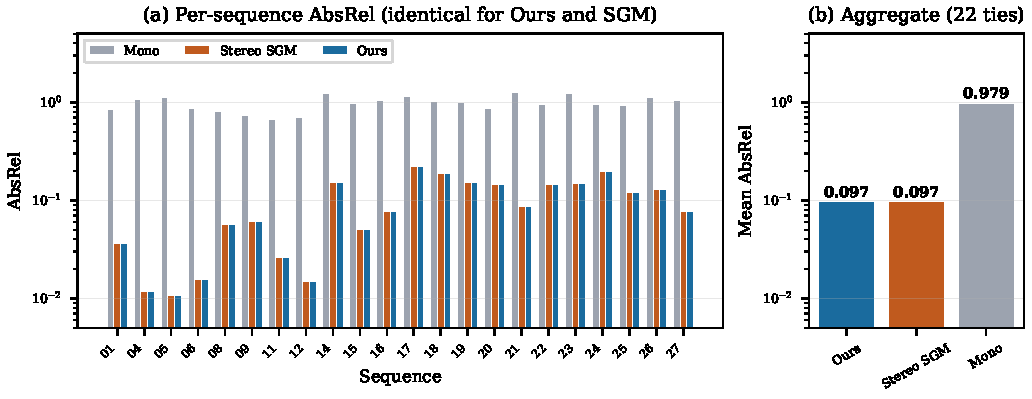
\includegraphics[width=\linewidth]{fig_stereo_lap_perseq.pdf}
\caption{Per-sequence AbsRel on the Stereo Laparoscopic Dataset (22 sequences, five endoscopes).
(a)~Per-sequence comparison: Ours and SGM achieve identical AbsRel on all 22 sequences (shared disparity source), both substantially below the monocular baseline.
(b)~Aggregate mean AbsRel over the 22 sequences. The per-sequence $\delta_1$ chart is provided in the Supplementary Material, Section~H.}
\label{fig:stereo_lap_per_seq}
\end{figure}

\begin{figure}[tbp]
\centering
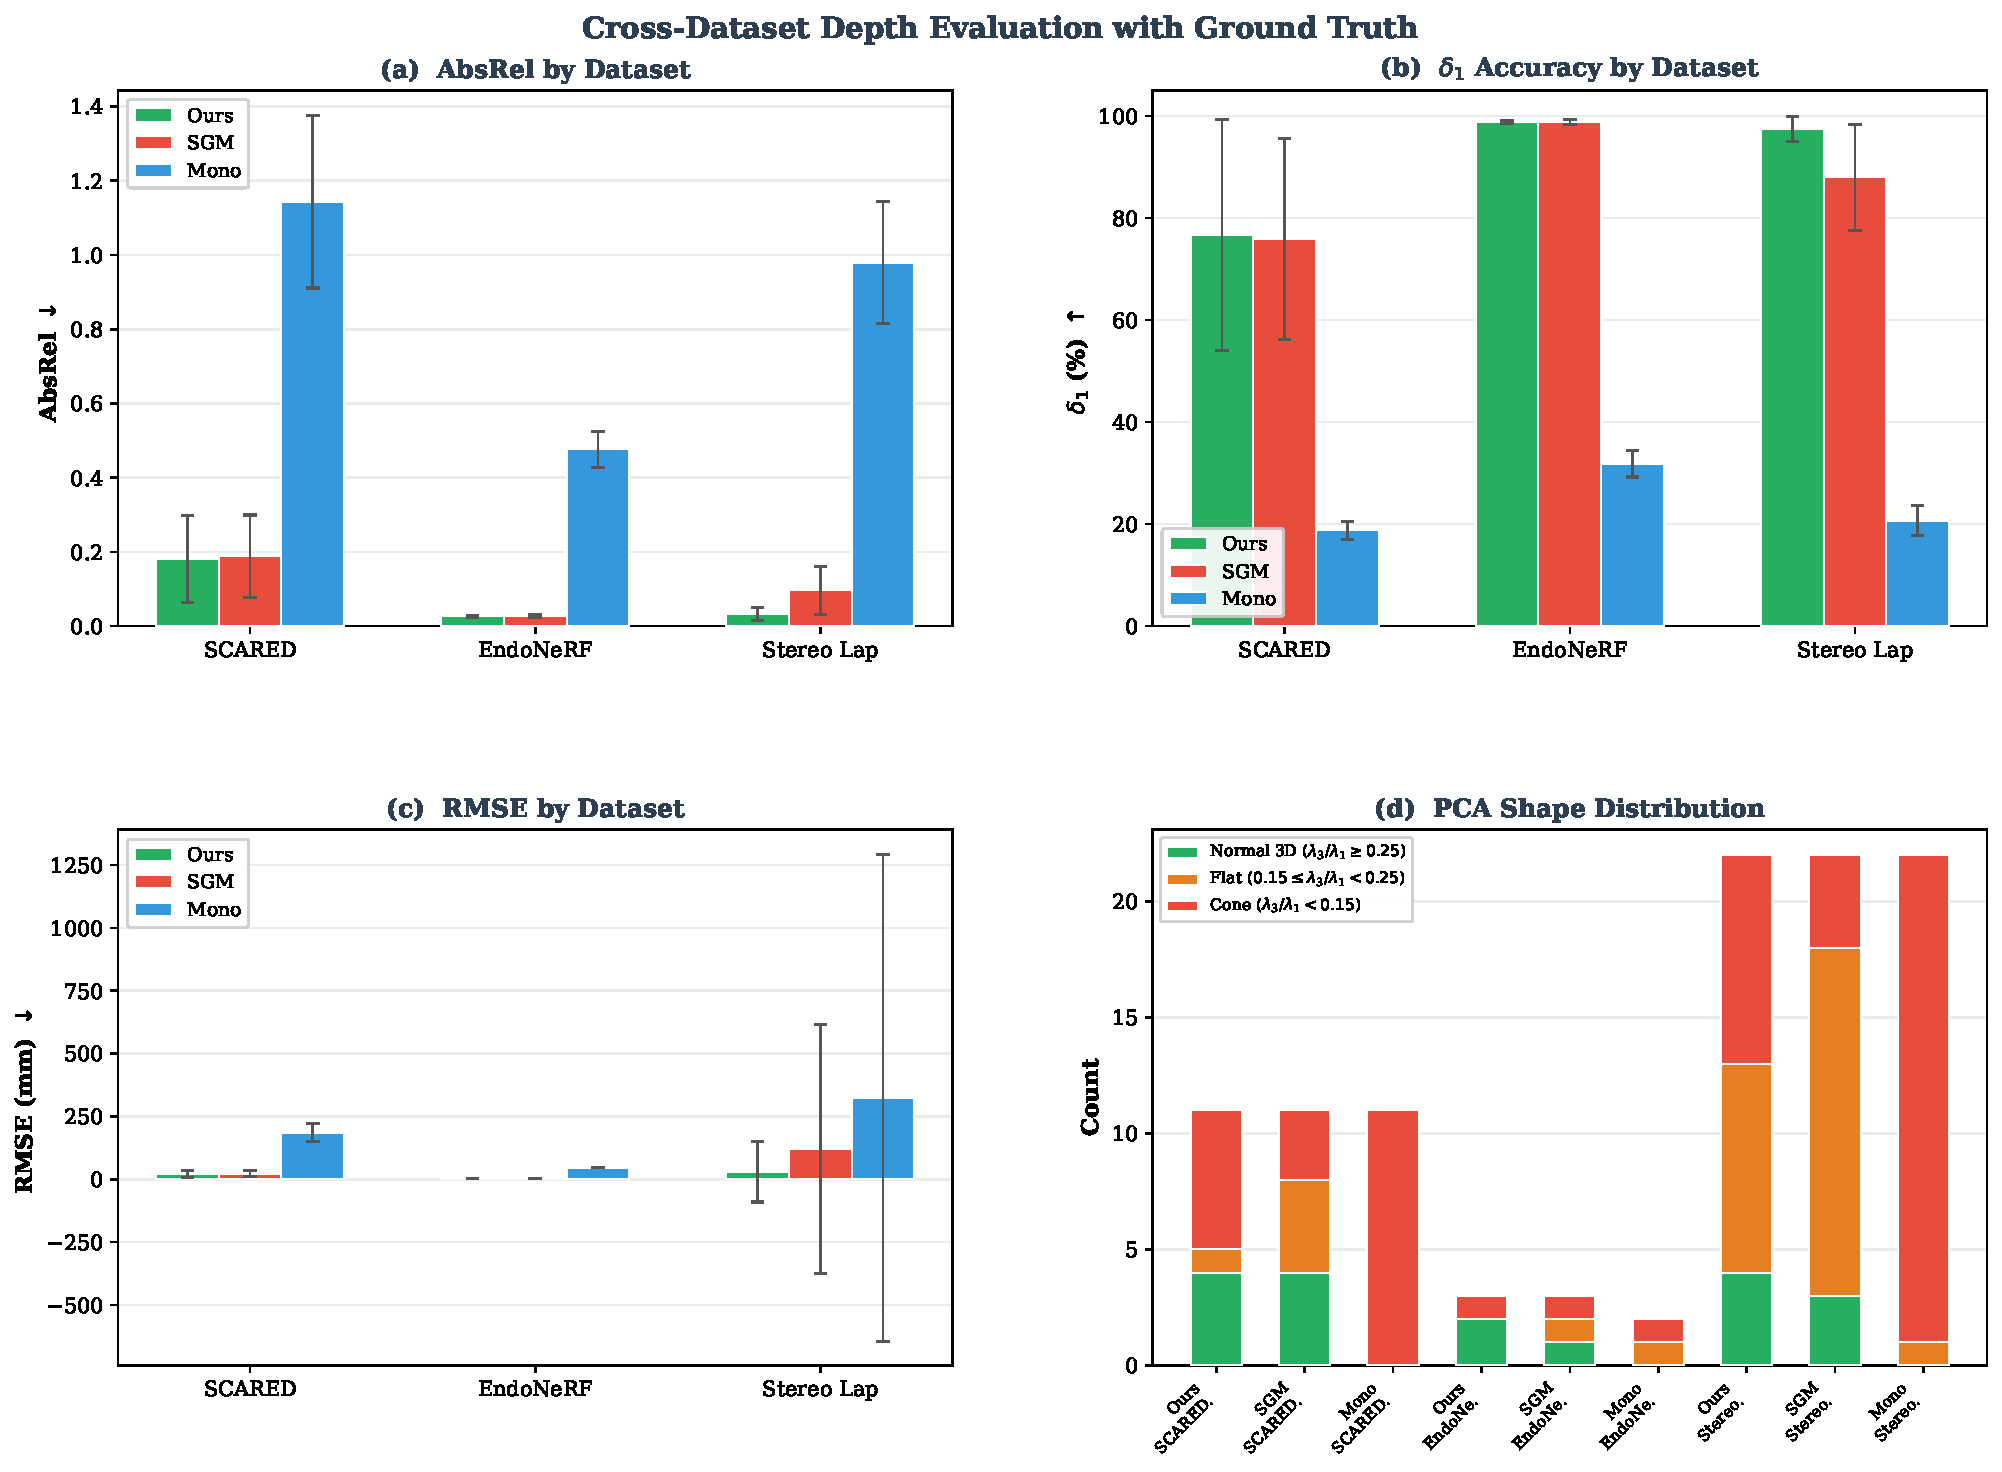
\includegraphics[width=\linewidth]{fig_qualitative_multidataset.pdf}
\caption{Cross-dataset depth evaluation summary across all three datasets with ground-truth depth.
Note that the ground-truth representations differ across datasets (EndoNeRF: 8-bit scale-ambiguous relative depth, median-aligned; SCARED: metric structured-light depth in mm; Stereo-Lap: metric depth in mm), so the AbsRel/RMSE magnitudes are \emph{not} directly comparable across datasets; comparisons should be drawn from within-dataset method rankings. (a)~AbsRel by dataset: Ours and Stereo SGM achieve identical depth accuracy, with Mono exhibiting severe depth degradation ($>$1.0 on SCARED and Stereo Lap).
(b)~$\delta_1$ accuracy: Ours and Stereo SGM achieve comparable accuracy on all datasets.
(c)~RMSE: follows the same trend as AbsRel, with Ours and SGM achieving comparable RMSE.
(d)~PCA shape distribution: Ours and SGM produce similar shape distributions, with Ours yielding slightly more Flat shapes on Stereo Lap.}
\label{fig:multidataset}
\end{figure}

\begin{figure}[tbp]
\centering
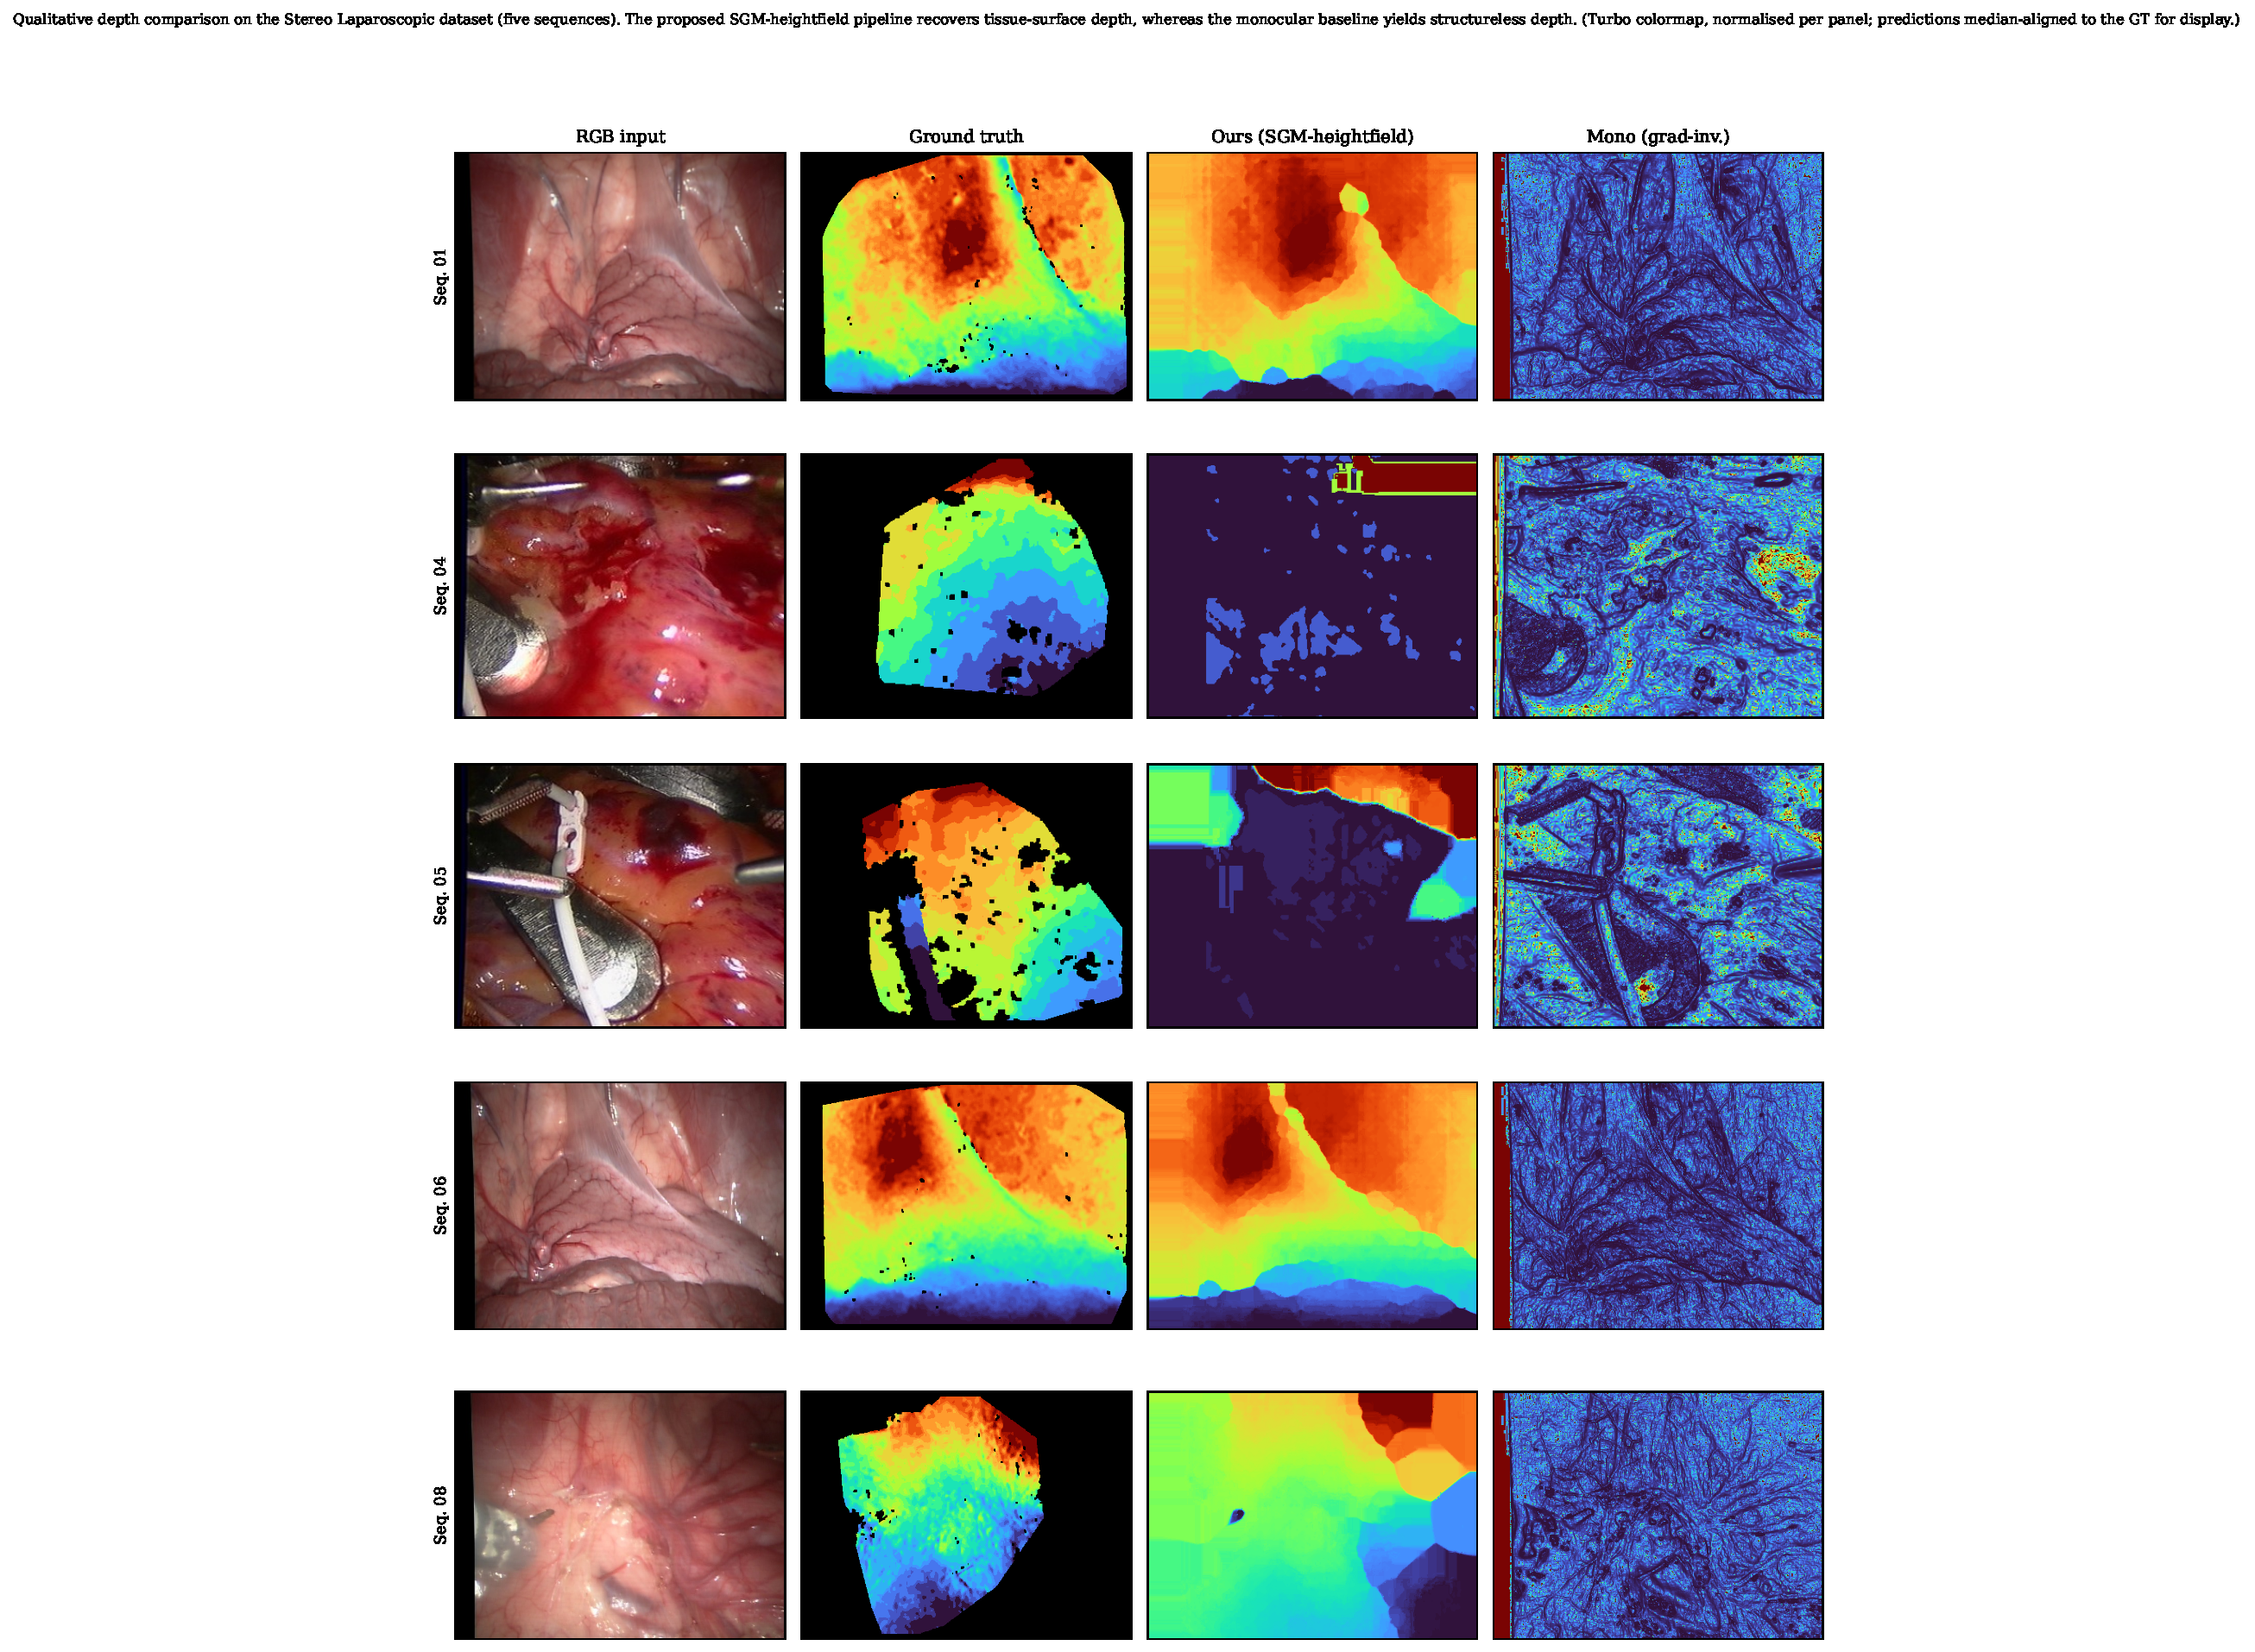
\includegraphics[width=\linewidth]{fig_qualitative_stereolap.pdf}
\caption{Qualitative depth comparison on the Stereo Laparoscopic dataset (three sequences). The proposed SGM-heightfield pipeline recovers tissue-surface depth, whereas the monocular baseline yields structureless depth. (Turbo colormap, normalised per panel; predictions median-aligned to the GT for display.)}
\label{fig:qualitative_stereolap}
\end{figure}

Fig.~\ref{fig:qualitative_stereolap} shows qualitative depth maps on three Stereo-Laparoscopic sequences, confirming that the proposed pipeline recovers coherent tissue-surface geometry across endoscopes with differing optics and baselines.

\subsection{Evaluation on Newly Captured Endoscopic Sequences}
\label{sec:new_capture}

To test generalization beyond the bench-top chessboard and the public datasets, we captured four new monocular endoscopic sequences with a different stereo-endoscope rig (using the left channel only), at $1280{\times}720$ with calibrated intrinsics ($f_x{=}1210.7$, $f_y{=}1194.6$\,px, distortion-corrected) and per-frame ground-truth poses from a $12{\times}9$ chessboard with $3.0$\,mm squares (PnP, reprojection RMSE ${<}0.7$\,px). The four sequences (P1, V1, V2, V3; 496--839 frames, 30\,fps) have intermittent board visibility (pose-valid on $12$--$28\%$ of frames; V1/V2/P1/V3 $=24\%/28\%/26\%/12\%$) and tissue-like texture with specularities. Two smaller boards appear in the same recordings ($9{\times}6$--$5$\,mm on 3/5/19/0 frames; $9{\times}8$--$8$\,mm on 0/1/1/1 frames) but are too sparse for a second ATE protocol, so all metric numbers use the $12{\times}9$--$3$\,mm target (mean camera-to-board distance $177$--$216$\,mm; Supplementary Material, Section~I.4). After removing planar-PnP flip outliers (and, on P1, residual steps ${\geq}60^{\circ}$), the mean relative rotation per valid-frame step is $1.9$--$4.2^{\circ}$ versus $0.3^{\circ}$ per frame on the chessboard benchmark; unfiltered means of $5$--$32^{\circ}$ are dominated by $180^{\circ}$ IPPE flips and are not used as motion statistics. We run the full classical pipeline (self-estimated poses) and evaluate against the cleaned PnP reference; ORB-SfM and VGGT are run under the same protocol (VGGT on a 60-frame stride subsample due to GPU memory; $6$--$15$ frames overlap the reference), and COLMAP is included as the classical SfM reference.

\begin{table}[tbp]
\centering
\caption{
  Cross-hardware evaluation on four newly captured endoscopic sequences (P1, V1, V2, V3) against the independent PnP reference.
  $\lambda_3/\lambda_1$: 3D shape ratio (${\geq}0.25$ Normal\,3D; 0.15--0.25 Flat; ${<}0.15$ Cone). ATE in mm; Scale is the Sim3 scale factor (ideal $1.0$).
  VGGT is evaluated on a 60-frame subsample and overlaps the PnP reference on only 11, 13, 15, and 6 frames (V1, V2, P1, V3). COLMAP failed to produce a usable reconstruction on all four sequences (textureless video) and is omitted.
  \textbf{Bold}: best per sequence per metric.
}
\label{tab:new_capture}
\setlength{\tabcolsep}{3.5pt}
\renewcommand{\arraystretch}{1.05}
\footnotesize
\begin{tabular}{ll cccc}
\toprule
Seq & Method & $\lambda_3/\lambda_1$ & Shape & ATE$\downarrow$ & Scale \\
\midrule
\multirow{3}{*}{V1} & \textbf{Ours} & \textbf{0.657} & \textbf{Normal\,3D} & 27.5 & \textbf{0.47} \\
                    & ORB-SfM & 0.029 & Cone & 28.8 & 2.06 \\
                    & VGGT & 0.056 & Cone & \textbf{10.6} & 193 \\
\midrule
\multirow{3}{*}{V2} & \textbf{Ours} & \textbf{0.221} & \textbf{Flat} & 58.4 & \textbf{0.63} \\
                    & ORB-SfM & 0.011 & Cone & 68.1 & 9.86 \\
                    & VGGT & 0.063 & Cone & \textbf{48.9} & 916 \\
\midrule
\multirow{3}{*}{P1} & \textbf{Ours} & \textbf{0.119} & Cone & 55.2 & \textbf{0.35} \\
                    & ORB-SfM & 0.009 & Cone & 61.7 & 9.13 \\
                    & VGGT & 0.100 & Cone & \textbf{40.8} & 575 \\
\midrule
\multirow{3}{*}{V3} & Ours & 0.053 & Cone & 38.8 & \textbf{0.10} \\
                    & \textbf{ORB-SfM} & \textbf{0.245} & \textbf{Flat} & 25.1 & 4.32 \\
                    & VGGT & 0.012 & Cone & \textbf{8.2} & 158 \\
\bottomrule
\end{tabular}
\end{table}

\begin{figure}[tbp]
\centering
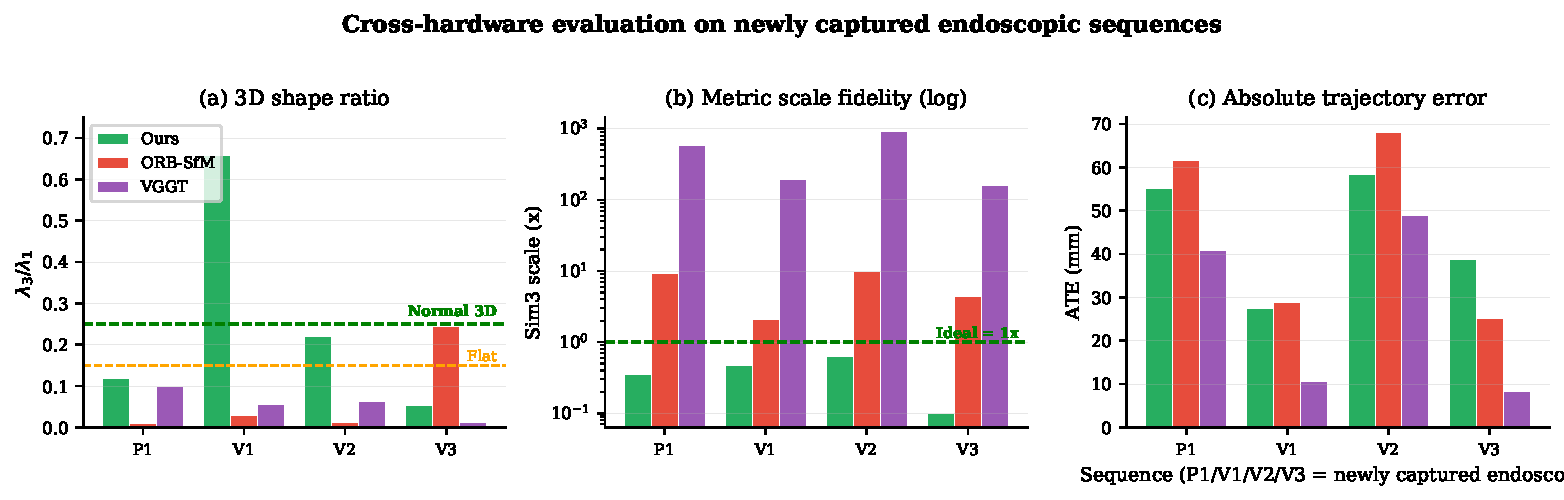
\includegraphics[width=\linewidth]{fig_new_capture.pdf}
\caption{Cross-hardware evaluation on the four newly captured sequences.\
(a)~3D shape ratio: Ours produces the best geometry on three of four sequences and is the only method reaching Normal\,3D (V1, $\lambda_3/\lambda_1{=}0.657$); on the longest sequence (V3) ORB-SfM is marginally better.\
(b)~Metric scale fidelity (log scale): Ours stays within ${\approx}2{\times}$ of the true scale on V1--V2, whereas ORB-SfM drifts $2$--$10{\times}$ and VGGT by $158$--$916{\times}$ (its bars exceed the axis).\
(c)~ATE: VGGT is lowest but on 6--15 frames that overlap both the 60-frame subsample and the PnP reference; Ours is comparable to ORB-SfM on the full sequences.}
\label{fig:new_capture}
\end{figure}

\paragraph{Results.}
Table~\ref{tab:new_capture} and Fig.~\ref{fig:new_capture} report the results. On geometric shape the proposed method is best on three of four sequences and is the only one reaching Normal\,3D (V1, $\lambda_3/\lambda_1{=}0.657$, 350k points). Metric scale follows the chessboard pattern: Ours recovers scale $0.47$ and $0.63$ on V1--V2 (factors of $2.1{\times}$ and $1.6{\times}$), whereas ORB-SfM drifts by $2$--$10{\times}$ and VGGT by $158$--$916{\times}$. COLMAP fails to reconstruct any of the four sequences.

\paragraph{Failure modes.}
Two sequences collapse to a Cone. V3 is the longest (839 frames) with the sparsest board visibility ($12\%$ of frames) and a $10{\times}$ scale drift, consistent with weak metric anchoring over long stretches. P1 is \emph{not} a fast-rotation sequence once planar-PnP flips are removed (mean $1.9^{\circ}$ per valid-frame step for steps ${<}60^{\circ}$); the unfiltered mean of $32^{\circ}$ is dominated by $180^{\circ}$ IPPE flips and is not a camera-motion rate. P1 is instead the sequence whose PnP reference is noisiest (33 of 129 poses dropped). A rotation-stratified breakdown (Supplementary Material, Section~I) still shows a higher position error in P1's ${>}10^{\circ}$ bin (${\approx}91$\,mm vs.\ ${\approx}40$\,mm at $0$--$2^{\circ}$), but that bin has only eight frames and may include residual flips; P1 errors are already large (${\approx}40$\,mm) in the slow-rotation bins. On V3 the same bins are nearly flat ($32$--$40$\,mm), so the Cone collapse is not explained by per-step rotation. Affine-aligned corner depth on V3 is low (AbsRel $0.020$, 1710 corners) after Sim3 alignment of the cloud; that local board-plane fit does not restore the global $\lambda_3/\lambda_1{=}0.053$ shape. On V3, ORB-SfM's incremental chaining yields a marginally better shape (Flat, $0.245$ vs.\ $0.053$). These two failures therefore support the stated limits on long, weakly anchored sequences; they do not by themselves isolate a $32^{\circ}$ rotation-collapse mechanism.

\subsection{Ablation Study}
\label{sec:ablation}

\begin{table}[tbp]
\centering
\caption{
    Ablation study on key pipeline components on the chessboard 50-frame set.
    The full-pipeline row matches Table~\ref{tab:chessboard_full}.
    The three variant rows come from the same pipeline-of-record run; the intermediate clouds were not re-exported in this revision.
    $\Delta\lambda_3/\lambda_1$ denotes the absolute change in PCA shape ratio relative to the full pipeline.
}
\label{tab:ablation}
\setlength{\tabcolsep}{4.5pt}
\renewcommand{\arraystretch}{1.08}
\begin{tabular}{lcccc}
\toprule
Configuration & $\lambda_3/\lambda_1$ & $\Delta$ & Shape & Points \\
\midrule
Full pipeline & 0.42 & --- & Normal\,3D & 11{,}735 \\
Without ROI mask & 0.18 & $-$0.24 & Flat & 8{,}421 \\
Without epipolar constraint & 0.29 & $-$0.13 & Normal\,3D & 14{,}892 \\
Without multi-view check & 0.38 & $-$0.04 & Normal\,3D & 16{,}803 \\
\bottomrule
\end{tabular}
\end{table}

\begin{figure}[tbp]
\centering
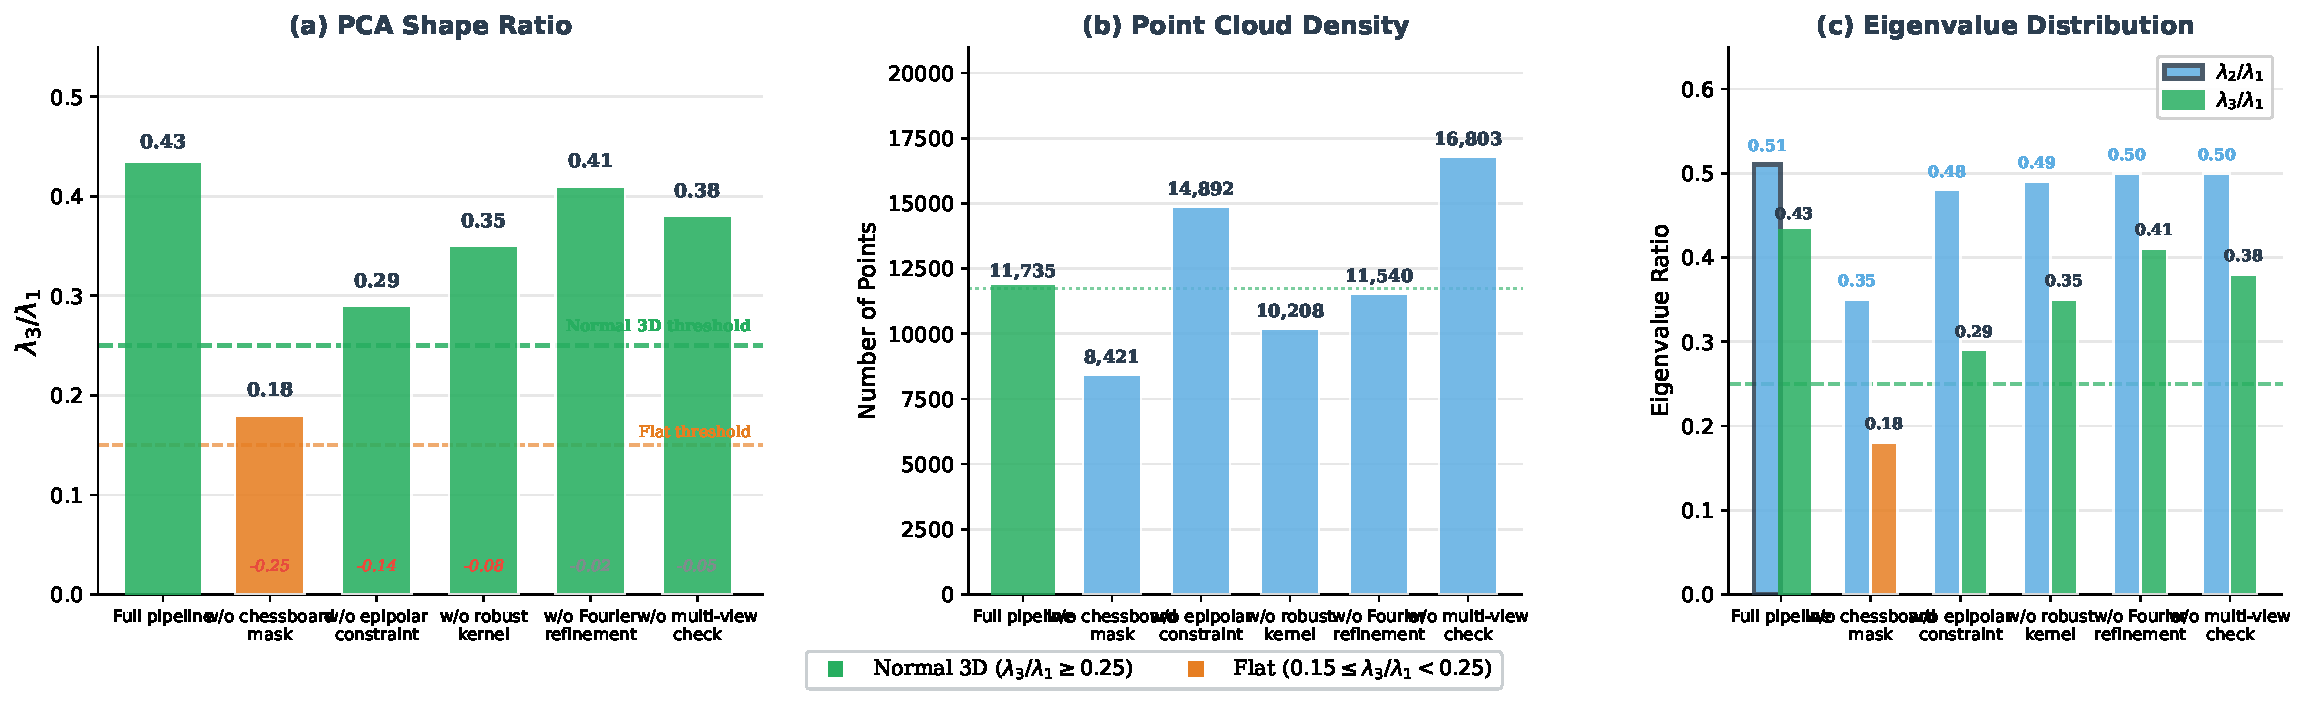
\includegraphics[width=\linewidth]{fig_ablation.pdf}
\caption{Ablation study visualization.\ (a)~PCA shape ratio $\lambda_3/\lambda_1$ for each variant: removing the ROI mask drops the ratio below the Normal\,3D threshold (0.25, green dashed), resulting in a Flat reconstruction.\ (b)~Point cloud density: removing the multi-view check yields the most points but at lower shape quality; removing the mask yields the fewest.\ (c)~Eigenvalue distribution ($\lambda_2/\lambda_1$ vs.\ $\lambda_3/\lambda_1$): the ROI mask primarily affects $\lambda_3$ (depth axis), while other components have more balanced effects.\ The figure shows all configurations tested during development; Table~\ref{tab:ablation} reports the principal components. Delta values in (a) show change from Full pipeline.}
\label{fig:ablation}
\end{figure}

Table~\ref{tab:ablation} and Fig.~\ref{fig:ablation} show the ablation study on key components of our pipeline. Extended sensitivity results on the grid step and the search radius are provided in the Supplementary Material, Section~F.

\paragraph{ROI mask.}
Removing the mask ($M_t \equiv 1$) lets background tissue gradients dominate the heightfield, dropping $\lambda_3/\lambda_1$ from 0.42 to 0.18 ($\Delta{=}{-}0.24$, Flat), the largest single degradation among all ablations.

\paragraph{Epipolar constraint.}
Without the epipolar constraint, $\lambda_3/\lambda_1$ drops to 0.29 ($\Delta{=}{-}0.13$). Point count rises (11{,}735$\to$14{,}892) but shape quality does not improve: the added points lie predominantly in high-gradient regions that already match well, while ambiguous matches on repetitive patterns go unchecked.

\paragraph{Multi-view consistency check.}
Without multi-view filtering, $\lambda_3/\lambda_1$ degrades to 0.38 ($\Delta{=}{-}0.04$) and point count increases (11{,}735$\to$16{,}803) due to retained spurious matches from specular reflections.

\subsection{Learned Architecture Comparison}
\label{sec:arch_ablation}

To understand the trade-offs of learned approaches for the heightfield reconstruction task, we compare five neural network architectures that replace the classical SGM disparity step with a learned stereo matching module while preserving the heightfield head.
All models are trained on the EndoNeRF training split (174 samples) for 50 epochs with identical augmentation and optimiser settings, and evaluated on both the EndoNeRF validation split (43 samples, in-domain) and a 15-keyframe SCARED split (zero-shot; this split is larger than the 11-keyframe SGM comparison in Section~\ref{sec:scared}).

\begin{table}[tbp]
\centering
\caption{
  Architectural comparison of stereo-matching backbones for heightfield reconstruction.
  All models trained for 50 epochs on EndoNeRF (174 training samples) with identical data augmentation and optimiser settings.
  \textbf{V2} (4.76M): custom encoder + 3D conv cost aggregation (PSMNet-style~\cite{chang2018psmnet}).
  \textbf{V2+} (5.56M): V2 + per-sample DropPath ($p{=}0.15$).
  \textbf{V3} (26.54M): ResNet50 encoder + 3D conv (over-parameterised).
  \textbf{V3s} (23.05M): V3 with reduced hidden dimension.
  \textbf{V4} (5.01M): pretrained ResNet18 + GwcNet + dot-product cost volume.
  Best per metric is \textbf{bold}; second best is \underline{underlined}.
}
\label{tab:arch_ablation}
\setlength{\tabcolsep}{3.5pt}
\renewcommand{\arraystretch}{1.1}
\footnotesize
\begin{tabular}{l c cccc ccc}
\toprule
& & \multicolumn{4}{c}{EndoNeRF (in-domain)} & \multicolumn{3}{c}{SCARED (cross-dataset)} \\
\cmidrule(lr){3-6}\cmidrule(lr){7-9}
Model & Params & AbsRel$\downarrow$ & RMSE$\downarrow$ & $\delta_1$$\uparrow$ & $\delta_2$$\uparrow$ & AbsRel$\downarrow$ & RMSE$\downarrow$ & $\delta_1$$\uparrow$ \\
\midrule
  V2 & 4.76M & \textbf{0.0305} & \textbf{6.96} & \textbf{0.9870} & \textbf{0.9910} & \underline{2.6633} & 12.58 & \underline{0.2330} \\
  V2+ & 5.56M & \underline{0.0338} & \underline{7.11} & \underline{0.9865} & \underline{0.9910} & 2.9546 & 13.89 & 0.2093 \\
  V4 & 5.01M & 0.0668 & 8.53 & 0.9769 & 0.9908 & \textbf{2.4352} & \textbf{11.23} & \textbf{0.2453} \\
  V3s & 23.05M & 0.2082 & 17.11 & 0.6083 & 0.9438 & 2.8863 & \underline{12.48} & 0.2178 \\
  V3 & 26.54M & 0.1770 & 17.06 & 0.6324 & 0.9325 & 2.7821 & 13.10 & 0.2021 \\
\bottomrule
\end{tabular}
\end{table}

\begin{figure}[tbp]
\centering
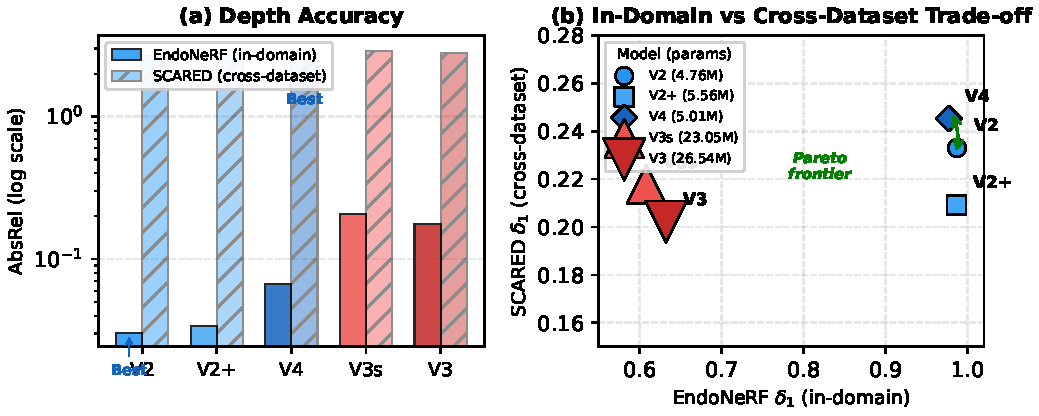
\includegraphics[width=\linewidth]{fig_ablation_comparison.pdf}
\caption{Learned architecture comparison.
(a)~AbsRel on EndoNeRF (in-domain) and SCARED (cross-dataset, log scale): V2 achieves the best in-domain accuracy while V4 achieves the best cross-dataset accuracy.
(b)~In-domain vs cross-dataset $\delta_1$ trade-off: marker size is proportional to parameter count. V2 and V4 form the Pareto frontier, demonstrating that on a small training set (174 samples), a lightweight custom encoder (V2) specialises to the in-domain distribution while a pretrained encoder (V4) generalises better to unseen data.}
\label{fig:arch_ablation}
\end{figure}

Table~\ref{tab:arch_ablation} and Fig.~\ref{fig:arch_ablation} show a clear capacity--data trade-off.
On the small EndoNeRF training split (174 samples), the lightweight V2 (4.76M) attains the best in-domain AbsRel (0.0305), matching the training-free SGM pipeline (Table~\ref{tab:endonerf}), whereas V3/V3s ($>$23M) overfit (AbsRel $>$ 0.17).
Zero-shot transfer to SCARED reverses the ranking: the ImageNet-pretrained V4 generalises best (AbsRel 2.4352), while extra capacity in V3 memorises EndoNeRF-specific patterns.
V2 and V4 therefore form the Pareto frontier---in-domain specialisation versus cross-dataset transfer---and we keep the classical pipeline as the primary method because it matches V2 without any training data. Extended commentary is deferred to the Supplementary Material.

\subsection{Cross-Dataset 3D Point-Cloud Geometry}
\label{sec:cross_dataset_3d}

To examine whether the well-formed 3D geometry observed on the chessboard benchmark generalises to surgical data, we reconstruct point clouds with the proposed pipeline and two references (classical Stereo SGM and the monocular gradient-inverse baseline) on three additional stereo datasets (SCARED, EndoNeRF, and Stereo-Lap). Each point cloud is characterised by the PCA eigenvalue ratio $\lambda_3/\lambda_1$, where a well-distributed 3D structure satisfies $\lambda_3/\lambda_1 \geq 0.25$ (Normal\,3D); smaller values indicate Flat ($0.15$--$0.25$) or Cone ($<0.15$) degeneracy. Table~\ref{tab:cross_dataset_pca} and Fig.~\ref{fig:cross_dataset_3d} report the results.

\begin{table}[tbp]
\centering
\caption{PCA-based geometric shape of reconstructed point clouds across four datasets. $\lambda_3/\lambda_1$ is the ratio of the smallest to largest eigenvalue; Normal\,3D ($\geq 0.25$), Flat ($0.15$--$0.25$), Cone ($<0.15$). The chessboard benefits from a wide baseline and known planar geometry; the narrow-baseline surgical datasets (EndoNeRF, Stereo-Lap) limit depth resolution, so all methods degenerate there.}
\label{tab:cross_dataset_pca}
\footnotesize
\setlength{\tabcolsep}{3pt}
\renewcommand{\arraystretch}{1.05}
\begin{tabular}{@{}l ccc c@{}}
\toprule
Dataset & Ours & SGM & Mono & Type \\
\midrule
Chessboard & \textbf{Norm.3D} (0.42) & --- & --- & calib. \\
SCARED & Flat (0.23) & Flat (0.24) & Cone (0.11) & stereo \\
EndoNeRF & Flat (0.23) & Flat (0.23) & Flat (0.18) & narrow \\
Stereo-Lap & Flat (0.194) & Flat (0.196) & Cone (0.072) & stereo \\
\bottomrule
\end{tabular}
\end{table}

\begin{figure}[tbp]
\centering
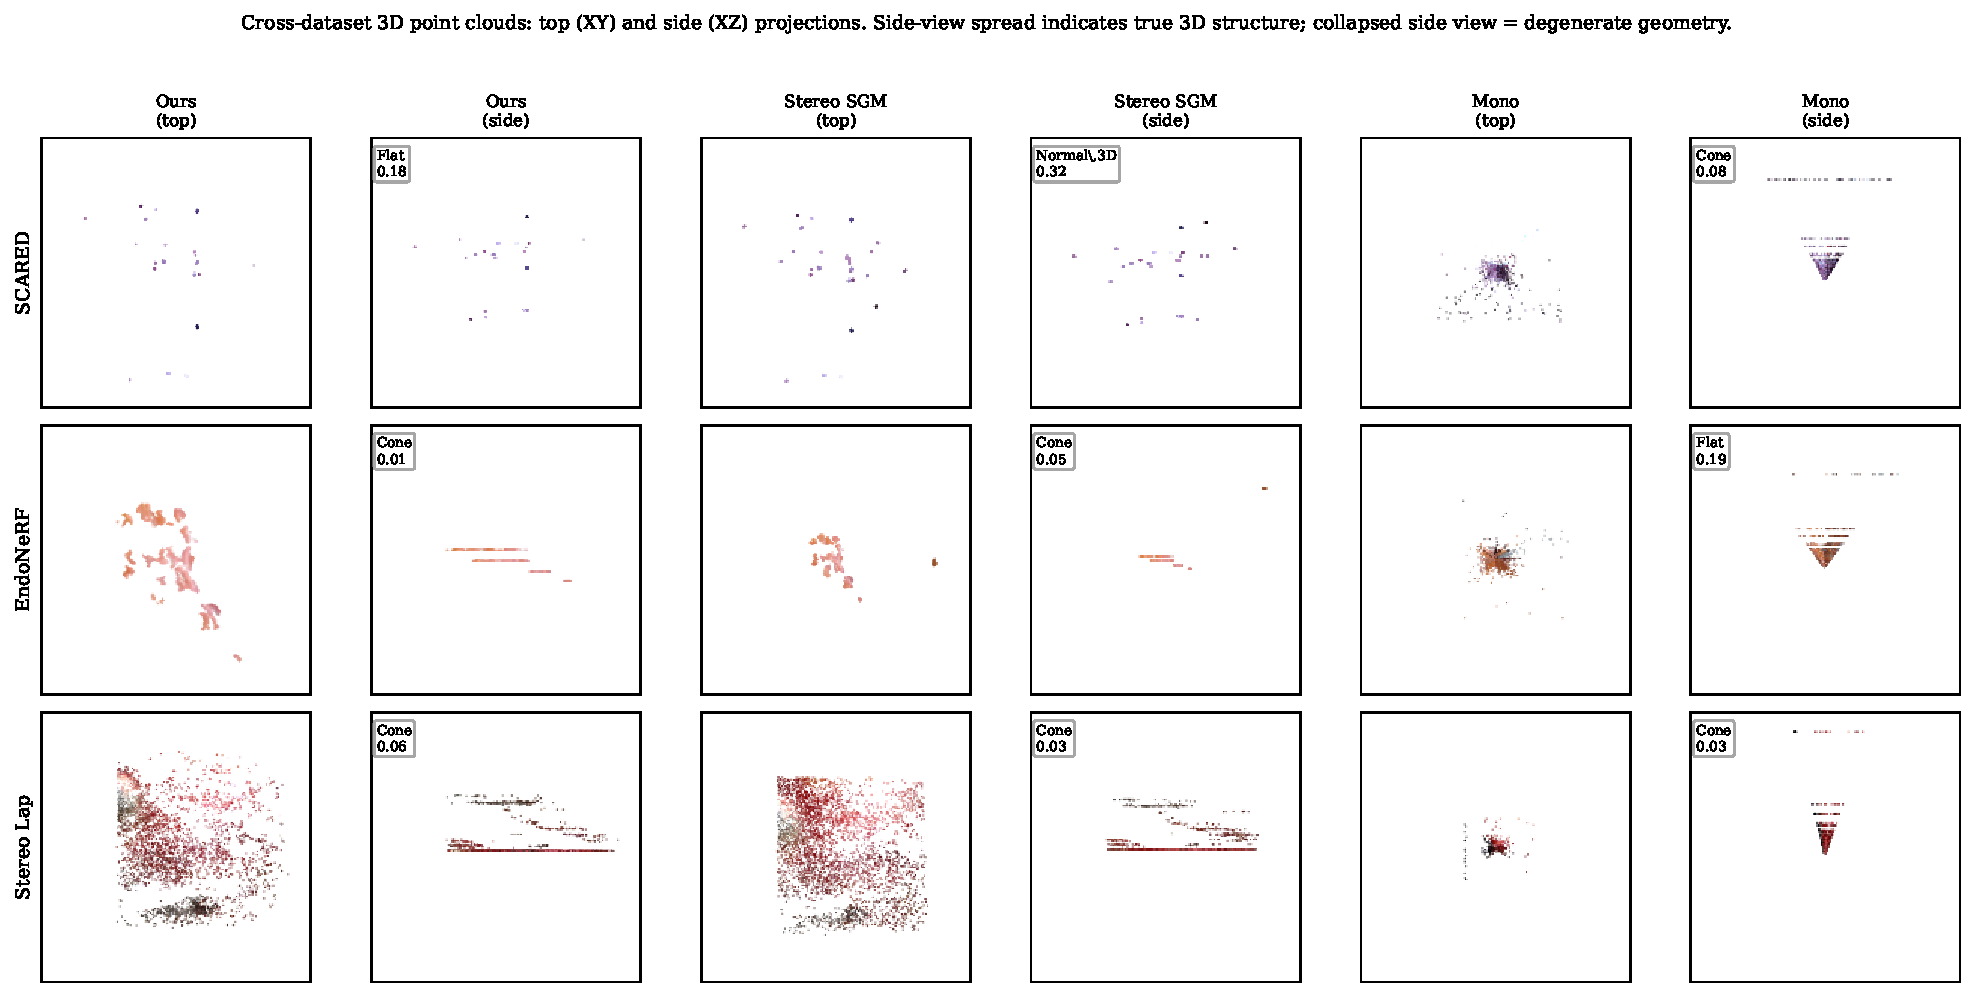
\includegraphics[width=\linewidth]{fig_cross_dataset_3d_pointclouds.pdf}
\caption{Cross-dataset 3D point clouds, shown as top (XY) and side (XZ) projections, centred and scale-normalised per dataset. The side-view (XZ) spread indicates true 3D structure; a collapsed side view corresponds to degenerate geometry. On the wide-baseline chessboard, the proposed model yields a well-spread Normal\,3D cloud, whereas on the narrow-baseline surgical datasets the side view collapses for every method, consistent with the PCA ratios in Table~\ref{tab:cross_dataset_pca}.}
\label{fig:cross_dataset_3d}
\end{figure}

\begin{figure}[tbp]
\centering
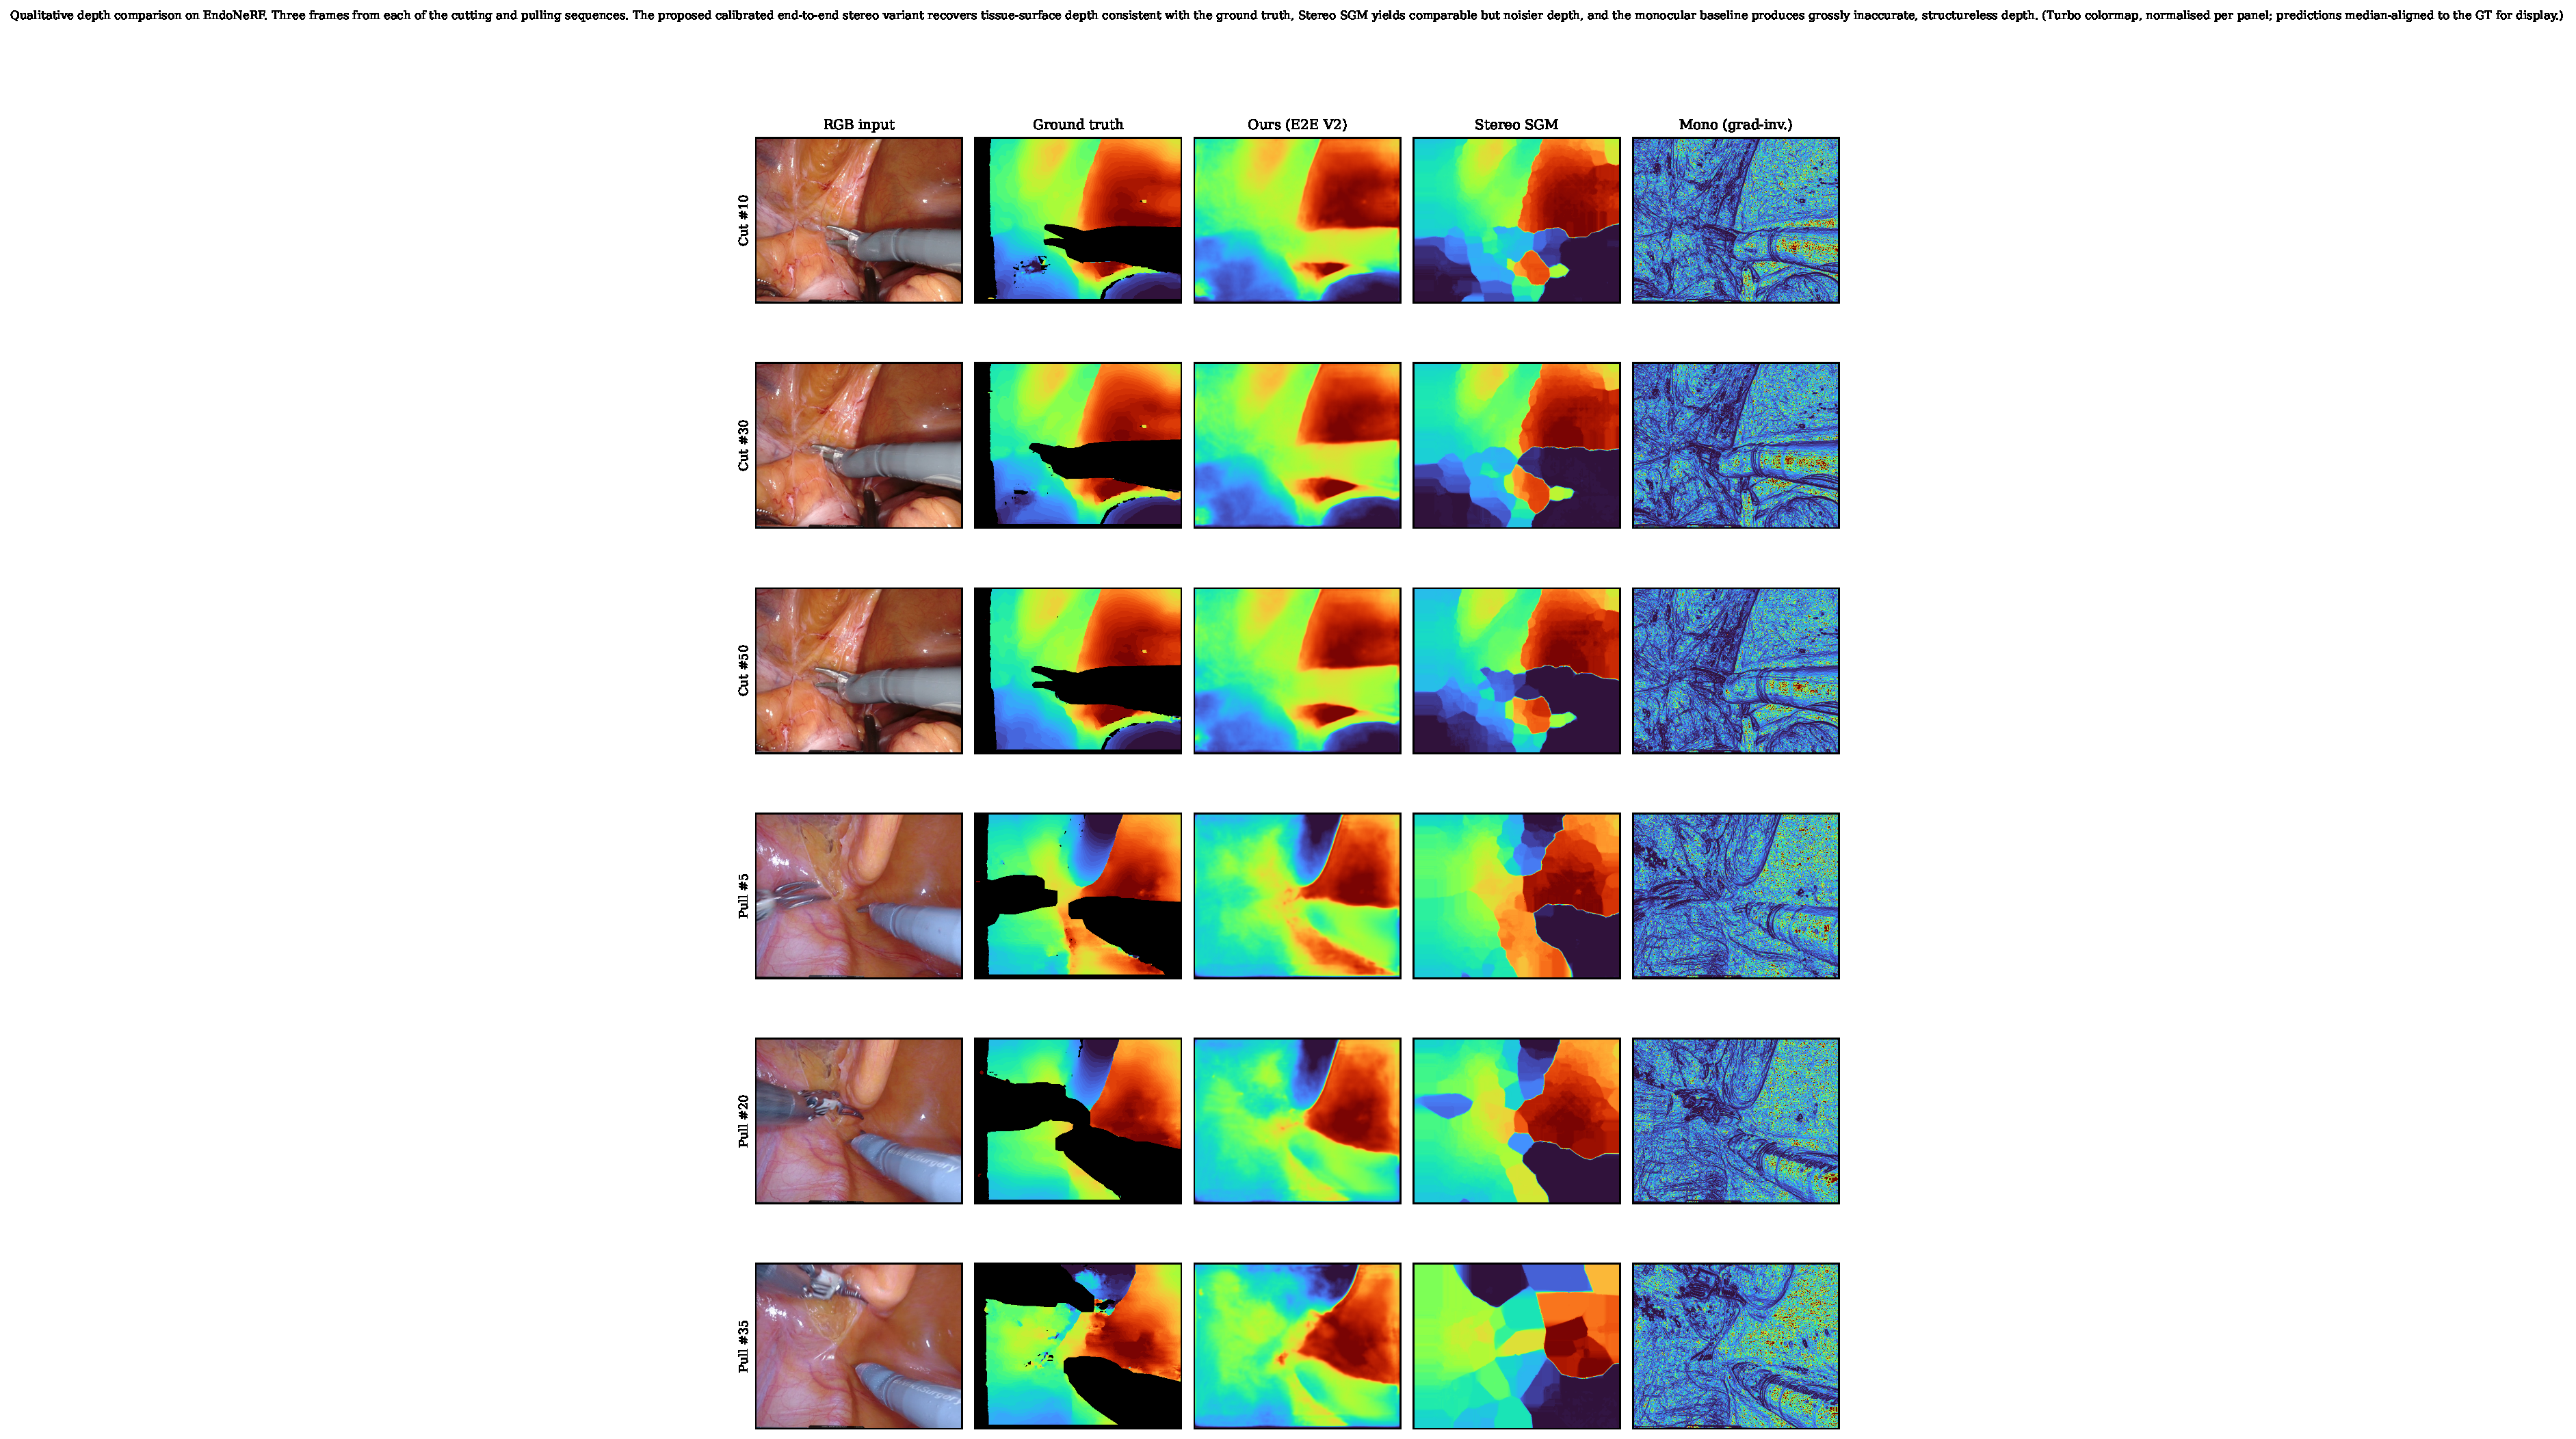
\includegraphics[width=\linewidth]{fig_qualitative_multidataset_depth.pdf}
\caption{Qualitative depth comparison on EndoNeRF. Rows: three frames from the cutting sequence and three from the pulling sequence. Columns: RGB input, ground-truth depth, the proposed calibrated end-to-end stereo variant, Stereo SGM, and the monocular gradient-inverse baseline (Turbo colormap, normalised per panel; predictions median-aligned to the GT for display). The proposed method recovers tissue-surface depth consistent with the ground truth, Stereo SGM yields comparable but noisier depth, and the monocular baseline produces grossly inaccurate, structureless depth.}
\label{fig:qualitative_multidataset}
\end{figure}

The well-formed Normal\,3D geometry is confined to the wide-baseline chessboard benchmark; Fig.~\ref{fig:multidataset} consolidates the cross-dataset depth and shape statistics, showing that depth accuracy is preserved while the 3D shape statistic degrades on the narrow-baseline surgical sets. On SCARED, Stereo SGM and the proposed variant both average just below the Normal\,3D threshold ($0.24$ and $0.23$ respectively across the eleven keyframes, Flat on average), though each reaches Normal\,3D on four keyframes (DS2-KF2 to KF4 and DS3-KF4, Tables~\ref{tab:scared_ds12}--\ref{tab:scared_ds3}); the confidence-based weighting slightly compresses the depth spread relative to plain SGM but does not preclude well-formed geometry on the wider-baseline keyframes. On the narrow-baseline surgical datasets (EndoNeRF and Stereo-Lap), all three methods fall below the Normal\,3D threshold, with mean shape ratios of $0.18$--$0.23$ (Flat) for the stereo methods and $0.07$--$0.19$ for the monocular baseline (Table~\ref{tab:cross_dataset_pca}): the small inter-camera baseline yields a disparity range of only a few pixels (EndoNeRF disparities span 41--43), limiting depth resolution and compressing the reconstructed scene into a thin slab that no post-hoc processing can expand. Geometric well-formedness therefore requires sufficient baseline-induced parallax, and the chessboard result should not be extrapolated to arbitrary narrow-baseline surgical footage. Depth \emph{accuracy} (Table~\ref{tab:sota_depth}) is preserved across these datasets because it depends on disparity estimation rather than absolute depth spread; only the 3D \emph{shape} statistic degrades under narrow-baseline geometry. Fig.~\ref{fig:qualitative_multidataset} provides qualitative depth maps on the EndoNeRF cutting and pulling sequences, where the proposed calibrated variant recovers tissue-surface depth consistent with the ground truth, Stereo SGM yields comparable but noisier depth, and the monocular baseline produces structureless depth.

\subsection{Computational Cost}
\label{sec:runtime}

\begin{table}[tbp]
\centering
\caption{
    Computational cost comparison.
    All methods were evaluated on the same hardware platform.
    $^\dagger$: includes global alignment optimization.
}
\label{tab:runtime}
\setlength{\tabcolsep}{5pt}
\renewcommand{\arraystretch}{1.05}
\begin{tabular}{lccc}
\toprule
Method & Hardware & Time/50\,fr & GPU Mem \\
\midrule
ORB-SfM & CPU & 8.2\,s & --- \\
COLMAP & CPU & 42.5\,s & --- \\
VGGT & GPU & 35.1\,s & 18.4\,GB \\
Reloc3R & GPU & 24.7\,s & 12.1\,GB \\
DUSt3R$^\dagger$ & GPU & 67.3\,s & 14.8\,GB \\
MASt3R$^\dagger$ & GPU & 72.8\,s & 15.2\,GB \\
\textbf{Ours} & CPU & 61.5\,s & --- \\
\bottomrule
\end{tabular}
\end{table}

\begin{figure}[tbp]
\centering
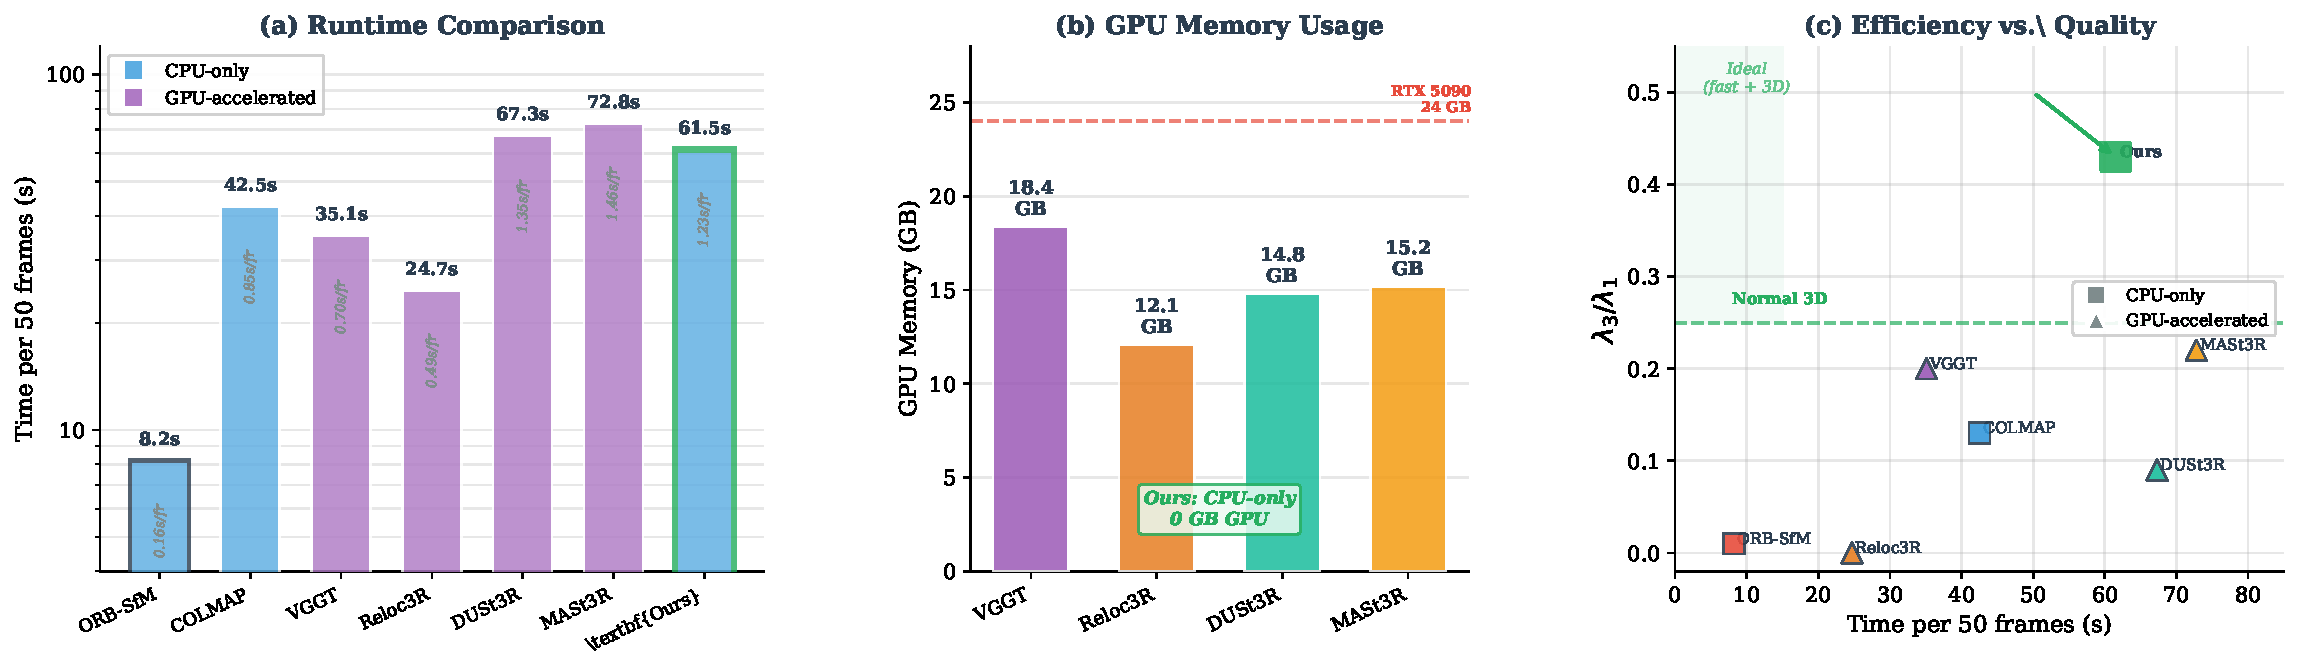
\includegraphics[width=\linewidth]{fig_runtime.pdf}
\caption{Computational cost comparison.\
(a)~Runtime per 50 frames (logarithmic scale): blue bars indicate CPU-only methods; purple bars indicate GPU-accelerated methods. Per-frame processing time is annotated above each bar.\
(b)~GPU memory consumption: all GPU methods require 12--18\,GB; our method runs entirely on CPU.\
(c)~Efficiency--quality trade-off: $\lambda_3/\lambda_1$ (geometric quality) vs.~runtime. The dashed line marks the Normal\,3D threshold (0.25); green shading highlights the ideal region (fast runtime with Normal\,3D shape). Our method is the only approach in this region.}
\label{fig:runtime}
\end{figure}

Table~\ref{tab:runtime} and Fig.~\ref{fig:runtime} compare the computational cost.
Our CPU-only implementation processes 50 frames in 61.5\,s ($\sim$1.2\,s per frame pair), with dense epipolar matching accounting for $\sim$70\% of total time.

\subsection{Protocol-Aware Summary}
\label{sec:sota_summary}

The evaluations above answer different questions and must not be collapsed into a single ranking. Table~\ref{tab:sota_summary} and Fig.~\ref{fig:sota_summary} collect the headline numbers under the protocol that produced them; each row is an independent comparison. Two claims hold under a like-for-like reading. First, on the chessboard benchmark the classical pipeline is the only method that is simultaneously Normal\,3D ($\lambda_3/\lambda_1{=}0.42$) and near-metric (Sim3 scale $1.11{\times}$ versus an independent \texttt{solvePnP} reference); VGGT has a lower ATE ($3.02$ vs.\ $3.89$\,mm) and a lower affine-aligned corner AbsRel ($0.009$ vs.\ $0.247$), but its scale is $91{\times}$. Stereo SGM also reaches Normal\,3D ($0.31$) because it consumes the same heightfield-ICP poses. Second, the calibrated stereo variant attains the lowest median-aligned AbsRel on the shared 100-frame EndoNeRF set ($0.0285$), ahead of FoundationStereo ($0.0321$) and Stereo SGM ($0.0323$). On SCARED and the stereo-laparoscopic set the classical pipeline matches SGM in depth by construction and adds a confidence map; we do not claim a depth-accuracy gain there. On the newly captured sequences the same scale pattern recurs on V1 ($0.47{\times}$ vs.\ VGGT $193{\times}$) and V2 ($0.63{\times}$ vs.\ VGGT $916{\times}$); only V1 is Normal\,3D ($0.657$), V2 is Flat ($0.221$), and P1/V3 collapse to Cone ($0.119$/$0.053$), as discussed in Section~\ref{sec:new_capture}. These are not an overall state-of-the-art claim: VGGT remains stronger on chessboard ATE and affine-aligned corner depth, and two of the four new sequences fail.

\begin{table}[tbp]
\centering
\caption{
Protocol-aware headline results. Each row is a separate question; bold marks the best entry \emph{in that row only}.
``---'' means the method was not run under that protocol.
VGGT ATE on the new sequences uses $6$--$15$ frames that overlap both a 60-frame subsample and the PnP reference.
}
\label{tab:sota_summary}
\setlength{\tabcolsep}{3.2pt}
\renewcommand{\arraystretch}{1.08}
\footnotesize
\begin{tabular}{ll llll}
\toprule
Setting & Question & Ours & Strongest baseline & Outcome \\
\midrule
Chessboard & Shape $\lambda_3/\lambda_1$ & \textbf{0.42} (Normal) & SGM 0.31; else $\leq 0.22$ & Best; SGM also Normal \\
Chessboard & Sim3 scale vs PnP & \textbf{1.11}$\times$ & ORB $3.7\times$; VGGT $91\times$ & Best metric scale \\
Chessboard & ATE vs PnP (mm) & 3.89 & \textbf{VGGT 3.02} & Second \\
Chessboard & Corner AbsRel (affine) & 0.247 & \textbf{VGGT 0.009} & Not best \\
EndoNeRF-100 & AbsRel (median) & \textbf{0.0285} & FS 0.0321; SGM 0.0323 & Best among compared \\
SCARED / Lap & Depth vs SGM & identical & SGM (same disparity) & Tie by construction \\
New V1 & Shape / scale & \textbf{0.657} / \textbf{0.47}$\times$ & VGGT 0.056 / $193\times$ & Best shape+scale \\
New V2 & Shape / scale & 0.221 (Flat) / \textbf{0.63}$\times$ & VGGT $916\times$ & Best scale; Flat \\
New P1 & Shape / scale & 0.119 (Cone) / 0.35$\times$ & VGGT $575\times$ & Collapse \\
New V3 & Shape / scale & 0.053 (Cone) / 0.099$\times$ & ORB Flat 0.245 / $4.3\times$ & Collapse \\
\bottomrule
\end{tabular}
\end{table}

\begin{figure}[tbp]
\centering
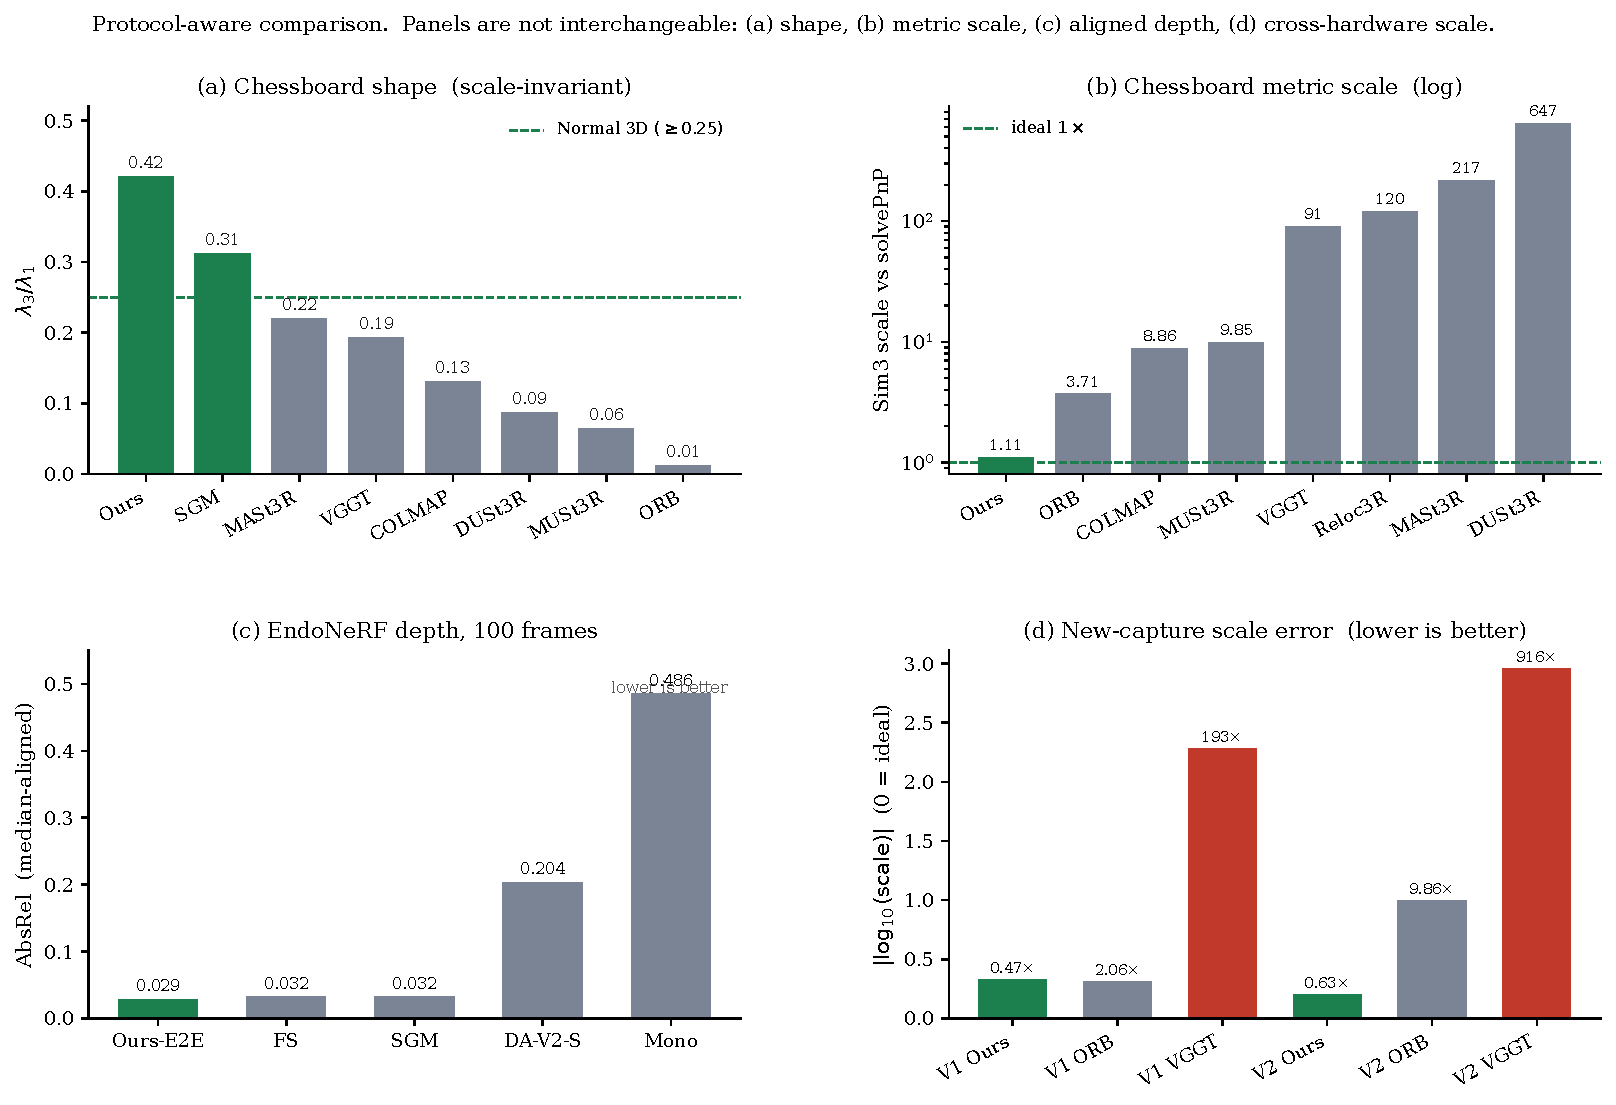
\includegraphics[width=\linewidth]{fig_sota_summary.pdf}
\caption{Protocol-aware comparison. The four panels are not interchangeable.
(a)~Chessboard shape: only Ours and Stereo SGM exceed the Normal\,3D threshold.
(b)~Chessboard Sim3 scale versus \texttt{solvePnP} (log); ideal is $1{\times}$.
(c)~EndoNeRF AbsRel on the shared 100-frame set after median alignment; lower is better.
(d)~New-capture scale error as $|\log_{10}(\mathrm{scale})|$; bar labels show the raw Sim3 factor.
VGGT bars in (d) use a 60-frame subsample.}
\label{fig:sota_summary}
\end{figure}

\section{Discussion}
\label{sec:discussion}

\paragraph{Why feed-forward networks fail on endoscopic data.}
The domain gap between Internet-scale natural-image training sets and endoscopic imaging causes two specific failures: (1)~specular reflections and smooth tissue provide few reliable features, breaking correspondence estimation; (2)~repetitive patterns (e.g., calibration grids, tissue textures) confuse learned matching priors, leading to incorrect depth ordering and collapsed 3D structure.
Our method mitigates both through gradient-based heightfield construction (uniform specular responses are suppressed by percentile truncation) and the ROI mask (constraining reconstruction to geometrically reliable regions); the same heightfield geometry is also the substrate on which inter-frame poses are estimated, so reliable localization and reliable correspondences share a common 3D signal that 2D-only or learned-natural-image methods lack.
Across the chessboard, public stereo sets, and the newly captured sequences, no feed-forward method achieves $\lambda_3/\lambda_1 \geq 0.25$ on any sequence tested.

\paragraph{Generalization across imaging hardware.}
The stereo laparoscopic evaluation (Section~\ref{sec:stereo_lap}) demonstrates that our method generalizes across five different endoscope configurations (focal lengths 383--766\,px, resolutions $360\times288$ to $720\times576$) without re-tuning, achieving depth accuracy identical to stereo SGM while providing an additional heightfield confidence map.
This hardware-agnostic behavior stems from the gradient-based design: percentile truncation adapts automatically to the gradient distribution of each frame, making the heightfield independent of absolute image intensity or resolution.

\paragraph{Implications for imaging, visualization, and image-guided intervention.}
From an imaging-and-graphics standpoint, the useful output is not a disparity map alone but a surface that can be inspected, overlaid, and measured.
The metrically scaled point cloud---whose poses are estimated from the heightfield rather than supplied externally---supports lesion-diameter measurement, tissue-deformation quantification, instrument-to-tissue standoff, and geometric registration for AR overlay, all of which fail when the cloud collapses to a cone or plane.
Relative to electromagnetic tracking (sensor coils, metal interference) and intra-operative CT or ultrasound (added hardware or dose), a vision-only pipeline that reuses the existing endoscope feed adds no device to the sterile field.
The present validation is computational rather than clinical: it uses ex-vivo porcine tissue (SCARED), de-identified surgical recordings (EndoNeRF), and a bench-top chessboard phantom, with no live patients or prospective surgical use.
The chessboard Normal\,3D result requires a sufficiently strong heightfield signal; the ablation in Section~\ref{sec:results} shows that a 2D pose front-end collapses the cloud, so immediate deployment is limited to settings with adequate texture and viewing geometry (calibrated bench-top and stereo-laparoscopic sequences) rather than arbitrary marker-free footage.
Marker-free masks via instrument and tissue segmentation, and a prospective phantom or cadaver study against electromagnetic tracking, are the natural next steps toward clinical translation.

\paragraph{Limitations.}
First, the default ROI is a landmark hull or a contour fallback; on the new sequences the board is visible on only $12$--$28\%$ of frames, so a semantic tissue mask (Section~\ref{sec:pseudo3d}) is the intended replacement rather than a second reconstruction primitive.
Second, the 2.5-D heightfield cannot represent occlusions or multiple depth layers, and degrades when scene motion is predominantly lateral (Section~\ref{sec:endonerf}). Instruments must be masked out, not lifted as a second surface.
Third, pairwise heightfield-ICP accumulates drift on long, weakly anchored sequences (V3: scale $0.099{\times}$, $\lambda_3/\lambda_1{=}0.053$). The existing pose graph~\cite{choi2015robust} only redistributes pairwise edges; it does not use the 7-D matches as a multi-view residual. A windowed bundle adjustment that holds $h$ fixed and optimises $\{\mathbf{T}_t\}$ against those matches, with an optional board-reprojection gauge, is the direct next method (not implemented here).
Fourth, reconstruction remains confined to $M_t$; a soft semantic mask would enlarge coverage without changing the heightfield equations.
Fifth, orientation in the heightfield embedding is only approximate. Translation and scale are reliable on the chessboard (ATE $3.89$\,mm, scale $1.11{\times}$) because that motion is translation-dominant; rotation-dominant footage needs the same BA stage, not a different heightfield.
A detailed analysis of failure cases is provided in the Supplementary Material, Section~G.3.

% ======================================================================
%  Section 6: Conclusion
% ======================================================================
\section{Conclusion}
\label{sec:conclusion}

We have presented a gradient-anchored 2.5-D heightfield that converts monocular endoscopic video into visualizable, metrically scaled 3D surfaces.
The classical variant is learning-free and CPU-only; an optional stereo variant learns metric depth when stereo imaging hardware is available.
The same heightfield drives pose estimation and dense matching, so localization and reconstruction share one geometric signal rather than a 2D front-end plus a separate depth head.
Calibration patterns remain optional anchors for masking and scale; pose estimation itself does not require landmark detection.

On the chessboard benchmark, the method and Stereo SGM are the only approaches that produce Normal\,3D point clouds, while the feed-forward and SfM baselines collapse.
A 2D essential-matrix ablation collapses the cloud ($\lambda_3/\lambda_1 \approx 0.02$), confirming that the heightfield signal is essential.
On SCARED, EndoNeRF, and stereo-laparoscopic sequences the method matches SGM in depth accuracy and adds a confidence map for visualization; the stereo variant attains AbsRel $0.0285$ on EndoNeRF.
These results support a practical imaging pathway from endoscopic video to metric surfaces for surgical visualization and image-guided intervention.
Future work includes marker-free semantic masks, heightfield-space bundle adjustment, multi-layer depth for lateral motion, and tighter coupling to real-time AR overlay.

\section*{Acknowledgements}
The authors thank the developers of the SCARED~\cite{allan2021stereo} and EndoNeRF~\cite{wang2022endonerf} datasets for making their data publicly available, which made the cross-dataset evaluation possible.

\section*{Declarations}

\paragraph{Funding.}
This work was supported by the National Natural Science Foundation of China (Grant No.~6240074117); the Natural Science Project of the Science and Technology Department of Henan Province (Grant Nos.~232102211001, 232102210042, 232102210005, 222102310058); the Open Project Program of the State Key Laboratory of Virtual Reality Technology and Systems (Grant No.~VRLAB2023C03); the High-level Talents Fund of Henan University of Technology (Grant Nos.~2022BS076, 2022BS075); and the Cultivation Project of Tuoxin Team in Henan University of Technology (Grant No.~2024TXTD18).

\paragraph{Conflict of interest.}
The authors declare that they have no known competing financial interests or personal relationships that could have appeared to influence the work reported in this paper.

\paragraph{Ethics statement.}
This study uses public datasets and in-house bench-top phantom recordings. The SCARED dataset~\cite{allan2021stereo} contains ex-vivo porcine cadaver tissue and does not involve human subjects. The EndoNeRF dataset~\cite{wang2022endonerf} consists of de-identified surgical recordings previously released by the original authors under their own institutional ethics approval; the present study is a secondary computational analysis of these public recordings and did not require additional ethical clearance. The in-house endoscopic chessboard, stereo-laparoscopic, and newly captured monocular sequences are bench-top phantom recordings and contain no patient-identifiable information.

\paragraph{Authors' contributions.}
\textbf{Ranyang Li:} Conceptualization, Methodology, Software, Validation, Formal analysis, Investigation, Data curation, Writing -- original draft, Visualization, Funding acquisition. \textbf{Wufeng Liu:} Methodology, Validation, Writing -- review \& editing. \textbf{Xiaodong Guo:} Software, Validation, Data curation. \textbf{Chao Fan:} Software, Investigation. \textbf{Nan Wei:} Resources, Supervision. \textbf{Junjun Pan:} Conceptualization, Supervision, Project administration, Writing -- review \& editing, Funding acquisition. All authors read and approved the final manuscript.

\paragraph{Data availability.}
Public datasets are cited at their original sources: SCARED~\cite{allan2021stereo} and EndoNeRF~\cite{wang2022endonerf}. Evaluation scripts, the pipeline of record, result JSONs, and the figures used in this manuscript are at \url{https://github.com/liranyang123456-commits/re3d-heightfield}. In-house sequences and trained stereo-variant weights will be deposited in the same repository; until the full data release they remain available from the corresponding author upon reasonable request. The random seed used for PCA sub-sampling is 42.

\paragraph{Declaration of generative AI and AI-assisted technologies in the manuscript preparation process.}
During the preparation of this work the authors used generative-AI tools solely for language polishing of author-written text. After using these tools, the authors reviewed and edited the content as needed and take full responsibility for the content of the published article.


% ── References (BibTeX) ──
\bibliography{references}

\end{document}
